% note.tex — スピノル QED：1ループの構造と検算（電子と μ 粒子、d = 4）
% コンパイル: lualatex note.tex（目次と参照の解決のため2〜3回）
\documentclass[a4paper,10pt]{ltjsarticle}
\usepackage[margin=20mm]{geometry}
\usepackage[haranoaji,deluxe]{luatexja-preset}
\ltjsetparameter{jacharrange={-3}}
\usepackage{amsmath,amssymb,slashed}
\usepackage{booktabs,tabularx,array}
\usepackage[table]{xcolor}
\usepackage{tikz}
\usetikzlibrary{arrows.meta,calc,positioning,decorations.markings,decorations.pathmorphing}
\usepackage[font=small,labelfont=bf]{caption}
\usepackage{graphicx}
\usepackage{placeins}
\usepackage{xurl}
\usepackage{hyperref}
\hypersetup{colorlinks=true,linkcolor=blue!50!black,citecolor=green!40!black,urlcolor=blue!60!black,
  pdftitle={Spinor QED with the electron and the muon: one-loop structure and tool checks},pdfauthor={}}

\renewcommand{\jsParagraphMark}{\textcolor{black!65}{\rule[-0.02\zw]{0.62\zw}{0.62\zw}}\hspace{0.35\zw}}
\newcommand{\dd}{\mathrm{d}}
\newcommand{\MSbar}{\overline{\mathrm{MS}}}
\newcommand{\DUV}{\Delta_{\mathrm{UV}}}
\newcommand{\DIR}{\Delta_{\mathrm{IR}}}
\newcommand{\sw}[1]{\langle #1\rangle}

\tikzset{
  photon/.style={thick,decorate,decoration={snake,amplitude=1.1pt,segment length=4.6pt}},
  fermion/.style={thick,postaction={decorate},
    decoration={markings,mark=at position 0.58 with {\arrow{Stealth[length=1.9mm]}}}},
  vtx/.style={circle,fill=black,inner sep=1.3pt},
  ctv/.style={circle,draw=black,fill=white,inner sep=0pt,minimum size=7pt,path picture={
      \draw (path picture bounding box.north west) -- (path picture bounding box.south east)
            (path picture bounding box.south west) -- (path picture bounding box.north east);}},
  mom/.style={-{Stealth[length=1.6mm]},thin},
  lab/.style={font=\small,align=center},
  blob/.style={circle,draw=black,fill=black!15,inner sep=0pt,minimum size=9pt},
  qdot/.style={rectangle,fill=black,inner sep=1.7pt},
  ml/.style={font=\scriptsize},
}

\title{スピノル QED：1ループの構造と検算（電子と $\mu$ 粒子、$d=4$）}
\author{}
\date{2026年10月13日}

\begin{document}
\maketitle

\begin{abstract}
$\phi^3$ 理論、$\phi^3+\phi^4$ 理論、擬スカラー湯川理論のノート~\cite{phi3note,phi34note,yukawanote} に続き、ゲージ場を含む最も簡単な模型として、電子 $e$ と $\mu$ 粒子の二つの Dirac フェルミオンが光子と結合するスピノル QED を $d=4$ で調べる。共変ゲージのゲージパラメータ $\xi$ を残し、紫外発散と赤外発散をともに次元正則化で扱い、紫外発散は $\MSbar$ で処理する。本ノートではまず、Feynman 則、Furry の定理、Ward--Takahashi 恒等式、1ループの1PI 関数（真空偏極、自己エネルギー、頂点）、$\MSbar$ の対抗項、繰り込み群の係数を手で求めた。フェルミオンの自己エネルギーは、部分積分の恒等式を使うと $D$ 次元で $\Sigma=\frac{e^2}{(4\pi)^2}[\xi(D-2)\slashed pB_1+(D-1+\xi)mB_0]$ という閉じた形になり、$\slashed p$ の項は $\xi$ に比例する（Landau ゲージでは1ループの場の繰り込みが0）。極質量はゲージによらず $m_{\mathrm p}=m(\mu)[1+\frac{e^2}{(4\pi)^2}(4+3\ln\frac{\mu^2}{m^2})]$ である。質量殻上の頂点は次元正則化では $\xi$ によらず、Feynman パラメータで二つの形状因子を閉じた形に書くと、$F_2(q^2)=\frac{2e^2m^2}{(4\pi)^2}\int_0^1\dd w/[m^2-q^2w(1-w)]$、とくに $F_2(0)=\alpha/2\pi$（Schwinger の値）となる。Ward 恒等式 $Z_1=Z_2$ により電荷の繰り込みは光子の場の繰り込みだけで決まり、二つのフレーバーで $\beta_e=8e^3/[3(4\pi)^2]$、$\mu\,\dd m/\dd\mu=-6e^2m/(4\pi)^2$ となる。$\MSbar$ の量を、極質量、留数、Thomson 極限の $\alpha(0)$ という on-shell の量に直す式も求めた。フェルミオンの留数は $\xi$ に依存する赤外の極を持ち、それを正しく得るには自己エネルギーの微分の $O(\epsilon)$ の項が要る。木のレベルでは、$e^+e^-\to\mu^+\mu^-$、Bhabha 散乱、Compton 散乱、$e^+e^-\to\gamma\gamma$ の振幅とスピン和を質量を残して求めた。1ループの $e^+e^-\to\mu^+\mu^-$ のうち $s$ チャンネルの部分（真空偏極、二つの頂点、外線の留数）は、$\MSbar$ で計算しても、$\alpha(0)$ と、処方によらない $F_1(q^2)-F_1(0)$、$\Pi(s)-\Pi(0)$、$F_2$ だけで書けることを示した。箱の図と木の干渉は、外線の Dirac 方程式で軟光子の項とそれ以外に分けて PaVe 関数の和に書いた。交差した箱は直接の箱の $t\leftrightarrow u$ の $-1$ 倍で、$\xi$ 依存は二つの箱の和で消え、干渉の赤外の極は外線の対ごとの軟光子の交換の和になる。この極は $D$ 次元の木のスピン和に掛かるので、$\MSbar$ の有限部分はスピン和の次元の規約により、4次元のスピン和との差は赤外の極の係数で閉じた形に書ける。最後に、検算と応用（異常磁気モーメント、走る結合と Landau 極、光子--光子散乱、Schwinger の対生成）の十一の手順を定め、その最初の四つを行った。FeynRules の模型ファイルから書き出した FeynArts と UFO の頂点、MadGraph の図の数は手計算と一致した。四つの過程の木の振幅とスピン和は、FeynCalc でも、Dirac 行列、スピノル、偏極ベクトルを陽に作った数値でも手計算と一致し、内線の光子のゲージパラメータに振幅がよらないこと、外線の光子についての Ward 恒等式も確かめた。MadGraph の断面積は三つの過程で統計誤差の1.5倍以内で一致したが、質量のある電子の Compton 散乱では $\sqrt s=4m_e$ で $1.5\%$ 小さかった。MadGraph の行列要素は正しく、後ろ向きの $u$ チャンネルの伝播関数の山を位相空間の積分で拾いきれないためで、その山を除くと一致する。1ループの1PI 関数は、一般の $\xi$ で FeynCalc の結果と記号として一致し、Furry の定理、光子4点関数の紫外の極の打ち消し、Ward--Takahashi 恒等式、$Z_1=Z_2$ も確かめた。有限部分と赤外の極は Package-X、LoopTools、COLLIER と相対 $2\times10^{-14}$ 以内で一致し、留数の赤外の極と $R_fF_1(0)=1$ も $\xi=0,1,3$ で確かめた。1ループの $e^+e^-\to\mu^+\mu^-$ では、FeynCalc で六つの図の干渉がそれぞれ手計算の式と記号として一致し、$\xi$ によらないこと、紫外の極が対抗項で消えることも確かめた。九つの物理的な点で、FeynCalc + LoopTools の値と手計算の式を COLLIER で評価した値は相対 $2\times10^{-14}$ 以内で、赤外の極は軟光子の交換の式と $4\times10^{-15}$ 以内で一致した。スピン和を4次元でとる FormCalc の有限部分は CDR と最大 $59\%$ ずれたが、規約の差を除くと $5\times10^{-15}$ 以内で一致した。箱の虚部は、$e^+e^-\to\gamma\gamma$ と $\mu^+\mu^-\to\gamma\gamma$ の木の振幅から作った二光子の中間状態の寄与と $6\times10^{-14}$ 以内で一致した（ユニタリー性）。導出はすべて付録に省略なく載せる。
\end{abstract}

\tableofcontents

\section{目的と問い}\label{sec:intro}

本ノートの問いは二つである。\textbf{第一に、ゲージ場とフェルミオンを含む最も簡単な繰り込み可能な模型で、$d=4$ の1ループの紫外発散と赤外発散、繰り込みの構造はどうなるか。そして、ゲージ対称性がその構造にどう現れるかを、これまでのノートと同じ手順でツールと突き合わせられるか。第二に、この模型の古典的な物理量を、同じ道具でどこまで再現し、拡張できるか。}具体的には、異常磁気モーメント、走る結合と Landau 極、光子--光子散乱、一様な電場での真空の崩壊（Schwinger の対生成）を調べる。

第一の問いを立てる理由は、これまでの三つのノート~\cite{phi3note,phi34note,yukawanote} がゲージ場を扱わず、ゲージ理論に固有の計算をツールで確かめる機会がなかったからである。ゲージ場を入れると、ゲージ固定とゲージパラメータ $\xi$、Ward--Takahashi 恒等式（真空偏極の横波性、頂点と自己エネルギーの対抗項の関係 $Z_1=Z_2$、電荷の繰り込みの普遍性）、光子の偏極の和、Furry の定理、光子4点関数の有限性が新たに現れる。光子に質量がないので、赤外発散と軟光子の放射による相殺（Bloch--Nordsieck）も現れる。フレーバーを二つにするのは、最も簡単な1ループの散乱である $e^+e^-\to\mu^+\mu^-$（$s$ チャンネルだけ）を扱うためと、真空偏極に質量の違う二つのループが入り、質量の取り違えをツールの検算で見つけられるようにするためである。第二の問いを立てる理由は、これらの量に精密な既知の結果があり、手計算とツールの両方の検証になるからである。Schwinger の対生成は、これまでのノートで作った bounce と前因子の道具の、フェルミオンとゲージ場への拡張になる。

求める量は五つである。(i) Feynman 則、Furry の定理、Ward--Takahashi 恒等式。(ii) 1ループの1PI 関数（光子とフェルミオンの2点関数、頂点）の紫外発散と $\MSbar$ の対抗項、光子3点・4点関数が発散しないこと。(iii) 繰り込まれた1PI 関数、繰り込み群の係数、$\MSbar$ から on-shell の量（極質量、留数、$\alpha(0)$）への換算。(iv) 四つの過程の木の振幅とスピン和、1ループの $e^+e^-\to\mu^+\mu^-$ とその S 行列要素、実の光子の放射を含む断面積。(v) 応用として、異常磁気モーメント、走る結合と Landau 極、光子--光子散乱、Schwinger の対生成。手計算とツールの間で求める一致は、これまでのノートと同じく、発散部分と対抗項では記号として完全な一致、有限部分では数値基準点での倍精度の一致である。

本ノートの構成は次の通りである。第~\ref{sec:setup} 節で模型と前提を定める。第~\ref{sec:results} 節で上の (i)〜(iv) の手計算の結果を述べる。第~\ref{sec:plan} 節で、これらと (v) を各ツールと突き合わせる計画を定める。第~\ref{sec:checks} 節で検算の結果を示す（現時点では手順 (1)〜(4)）。第~\ref{sec:discussion} 節で次の手順をまとめる。導出は\ref{app:rules}〜\ref{app:scat} に、検算の細部は\ref{app:details} にある。

\section{設定}\label{sec:setup}

模型は、光子 $A_\mu$ と、質量 $m_e$、$m_\mu$ の二つの Dirac フェルミオン $\psi_e$、$\psi_\mu$ からなる理論である。ラグランジアン密度は
\begin{equation}
\begin{aligned}
\mathcal{L}={}&-\frac14F_{\mu\nu}F^{\mu\nu}-\frac{1}{2\xi}\bigl(\partial_\mu A^\mu\bigr)^2
+\sum_{f=e,\mu}\Bigl[\bar\psi_f\bigl(i\slashed\partial-m_f\bigr)\psi_f+e\mu^{\epsilon}Q_f\,\bar\psi_f\gamma^\mu\psi_f\,A_\mu\Bigr]\\
&-\frac14\,\delta_3F_{\mu\nu}F^{\mu\nu}
+\sum_{f=e,\mu}\Bigl[\delta_2^f\,\bar\psi_f\,i\slashed\partial\,\psi_f-\bigl(\delta_2^f+\delta_m^f\bigr)m_f\bar\psi_f\psi_f+\delta_1^f\,e\mu^{\epsilon}Q_f\,\bar\psi_f\gamma^\mu\psi_f\,A_\mu\Bigr]
\end{aligned}
\label{eq:L}
\end{equation}
とする。$F_{\mu\nu}=\partial_\mu A_\nu-\partial_\nu A_\mu$、$Q_e=Q_\mu=-1$ である。1行目は共変微分 $D_\mu=\partial_\mu-ie\mu^\epsilon Q_fA_\mu$ を使って $\bar\psi_f(i\slashed D-m_f)\psi_f$ と書いたものに、ゲージ固定の項を加えたものである。2行目が対抗項で、裸の量と
\begin{equation*}
A_0=Z_3^{1/2}A,\quad \psi_{f,0}=(Z_2^f)^{1/2}\psi_f,\quad m_{f,0}=Z_m^fm_f,\quad e_0=Z_e\mu^\epsilon e,\quad \xi_0=Z_3\,\xi,\qquad
Z_1^f\equiv Z_eZ_2^fZ_3^{1/2}
\end{equation*}
で結ばれる。$\delta_i\equiv Z_i-1$ で、1ループの次数では $Z_2Z_m-1=\delta_2+\delta_m$ である。$\xi_0=Z_3\xi$ とするので、ゲージ固定の項 $(\partial A_0)^2/\xi_0=(\partial A)^2/\xi$ には対抗項が付かない。

\paragraph{前提。}本ノートは次の前提に立つ。
\begin{enumerate}
\item 計量は $(+,-,-,-)$、$\hbar=c=1$ とする。$\slashed a\equiv\gamma^\mu a_\mu$、$\sigma^{\mu\nu}\equiv\frac i2[\gamma^\mu,\gamma^\nu]$ である。
\item 場は光子と、電荷 $Q_f=-1$ の二つの Dirac フェルミオン（$f=e,\mu$）とし、相互作用はゲージ結合だけとする。$e>0$ で、共変微分の符号は FeynRules の規約 $D_\mu=\partial_\mu-ieQ_fA_\mu$ に合わせる。$m_e,m_\mu>0$ である。フレーバーの数は $N_f\equiv\sum_fQ_f^2=2$ である。
\item ゲージは共変ゲージで、ゲージパラメータを $\xi$ とする（$\xi=1$ が Feynman ゲージ、$\xi=0$ が Landau ゲージ）。可換ゲージ理論なので Faddeev--Popov のゴーストは他の場と結合せず、省く。物理量は $\xi$ によらないはずで、それを確かめる。
\item 時空次元は $d=4$ とする。ループ積分は次元正則化で行い、$D=4-2\epsilon$ とする。光子に質量がないので赤外発散が生じるが、それも同じ $D$ 次元で正則化する。紫外と赤外の極は同じ $1/\epsilon$ だが、由来を示したいときは $\DUV$、$\DIR$ と書き分ける（数値としては等しい）。$\gamma$ 行列は $D$ 次元で反可換で、$\mathrm{tr}\,1=4$ とする（$\gamma^5$ は現れない）。
\item 紫外発散は $\MSbar$ で処理する。すなわち、対抗項を $\DUV\equiv1/\epsilon-\gamma_E+\ln4\pi$ に比例させる。赤外の極も $\DIR\equiv1/\epsilon-\gamma_E+\ln4\pi$ の形にまとめる。$e(\mu)$、$m_f(\mu)$ は $\MSbar$ の走る量で、on-shell の量（$\alpha(0)$、極質量）はそこから換算する。
\item 数値を比べるときの基準点は $e=1$、$m_e=\mu=1$、$m_\mu=1.7$、$\xi=1$ とし、ゲージの検算では $\xi=0,3$ も使う（質量と $\mu$ は $m_e$ を単位とする）。応用の手順では、物理の値 $\alpha^{-1}(0)=137.035999$、$m_\mu/m_e=206.768283$ を使う。
\end{enumerate}
本文で使う記号を表~\ref{tab:notation} にまとめる。

\begin{table}[tbp]
\centering\small
\caption{本ノートで使う記号。}
\label{tab:notation}
\begin{tabularx}{\linewidth}{>{\raggedright\arraybackslash}p{3.7cm}X}
\toprule
\textbf{記号} & \textbf{意味} \\
\midrule
$A_\mu$ & 光子の場（模型ファイル \texttt{Src/SpinorQED.fr} の \texttt{A}） \\
$\psi_f$, $m_f$, $Q_f$ & フレーバー $f=e,\mu$ の Dirac フェルミオン、その（$\MSbar$ の）質量、電荷 $Q_f=-1$（\texttt{elec}、\texttt{muon}、\texttt{Me}、\texttt{MMU}） \\
$e$, $\alpha$ & 電荷の単位（\texttt{ee}）と $\alpha\equiv e^2/4\pi$。とくに断らなければ $\MSbar$ の $e(\mu)$ \\
$\xi$ & 共変ゲージのゲージパラメータ \\
$N_f$ & $\sum_fQ_f^2=2$ \\
$D$, $\epsilon$, $K$ & 正則化した次元 $D=4-2\epsilon$、そのずれ、$K\equiv(4\pi)^2$ \\
$\mu$ & 繰り込みスケール（$\MSbar$ のスケール） \\
$\DUV$, $\DIR$ & 紫外と赤外の極 $1/\epsilon-\gamma_E+\ln4\pi$。数値としては等しい \\
$\delta_3,\ \delta_2^f,\ \delta_m^f,\ \delta_1^f$ & 光子の場・フェルミオンの場・フェルミオンの質量・頂点の対抗項（$\MSbar$）。$Z_i=1+\delta_i$ \\
$S_f(p)$ & フェルミオンの伝播関数の行列 $(\slashed p-m_f)^{-1}=(\slashed p+m_f)/(p^2-m_f^2+i0)$ \\
$D_{\nu\rho}(l)$ & 光子の伝播関数の行列 $[g_{\nu\rho}-(1-\xi)l_\nu l_\rho/l^2]/l^2$（伝播関数は $-iD_{\nu\rho}$） \\
$\Pi^{\mu\nu}$, $\Pi_f$ & 光子の1PI 2点関数 $i\Pi^{\mu\nu}=i(q^2g^{\mu\nu}-q^\mu q^\nu)\Pi(q^2)$ と、フレーバー $f$ のループの寄与 $\Pi_f$。$\Pi=\sum_f\Pi_f$ \\
$\Sigma_f$, $\Sigma_V$, $\Sigma_S$ & フェルミオンの自己エネルギー（1PI 2点関数が $-i\Sigma$）と、その分解 $\Sigma=\slashed p\,\Sigma_V(p^2)+m\,\Sigma_S(p^2)$ \\
$\Lambda^\mu$ & 頂点の補正。1PI 3点関数を $ieQ_f[\gamma^\mu+\Lambda^\mu(p',p)]$ と書く（$p$ が入るフェルミオン、$p'=p+q$ が出るフェルミオン） \\
$F_1$, $F_2$ & 質量殻上の頂点の形状因子 $\bar u(p')[\gamma^\mu F_1+\frac{i\sigma^{\mu\nu}q_\nu}{2m}F_2]u(p)$。$F_1^\Lambda$ は $\Lambda^\mu$ だけの寄与 \\
$\hat F_1$, $\hat\Pi$ & 処方によらない組 $\hat F_1(q^2)\equiv1+F_1^\Lambda(q^2)-F_1^\Lambda(0)$、$\hat\Pi(q^2)\equiv\Pi(q^2)-\Pi(0)$ \\
$f_{\mathrm{IR}}(q^2)$ & $\hat F_1$ の赤外の極の係数（式~\eqref{eq:fir}） \\
$A_0,\ B_0,\ B_1,\ C_0$ & 1ループ積分（LoopTools の規約）。式~\eqref{eq:IN} の $(K/i)$ 倍で、$\MSbar$ の有限部分は $\DUV=0$ の値。$B_n(p^2;m_1^2,m_2^2)$ \\
$\dd F$, $\Delta_F$, $h(w)$ & Feynman パラメータの測度 $\dd x\,\dd y\,\dd z\,\delta(x+y+z-1)$、頂点の分母 $\Delta_F=(1-z)^2m^2-xyq^2$、$h(w)=m^2-q^2w(1-w)$ \\
$m_{f,\mathrm p},\ R_f,\ R_A$ & フェルミオンの極質量と留数、光子の留数（式~\eqref{eq:os}） \\
$e_{\mathrm{OS}}$, $\alpha(0)$ & Thomson 極限で定めた電荷と $\alpha(0)=e_{\mathrm{OS}}^2/4\pi$ \\
$\beta_e,\ \gamma_m^f,\ \gamma_\psi,\ \gamma_A$ & $\beta_e\equiv\dd e/\dd\ln\mu$、$\gamma_m^f\equiv\mu\,\dd m_f/\dd\mu$、$\gamma_\psi\equiv\frac12\dd\ln Z_2/\dd\ln\mu$、$\gamma_A\equiv\frac12\dd\ln Z_3/\dd\ln\mu$ \\
$s,\ t,\ u$ & Mandelstam 変数 \\
$\mathcal M_A,\dots,\mathcal M_D$ & $e^+e^-\to\mu^+\mu^-$、$e^+e^-\to e^+e^-$、$e^-\gamma\to e^-\gamma$、$e^+e^-\to\gamma\gamma$ の振幅（式~\eqref{eq:Mtree}） \\
$\sum|\mathcal M|^2$ & 外線のフェルミオンのスピンと光子の偏極についての和（平均ではない） \\
$W$, $B(D)$ & 木と1ループの $e^+e^-\to\mu^+\mu^-$ の振幅の干渉 $\sum\mathcal M_A^*\mathcal M^{(1)}$ と、$D$ 次元の木のスピン和 $\sum|\mathcal M_A|^2$（式~\eqref{eq:Wbox}） \\
$\mathcal N(s,t)$, $G(x)$, $\tau$ & 直接の箱の干渉の積分（表~\ref{tab:box}）、箱の赤外の極の関数（式~\eqref{eq:Wir}）、$\tau=m_e^2+m_\mu^2-t$ \\
$E_\gamma,\ E_\psi,\ L$ & 図の外の光子線、外のフェルミオン線の数、ループの数 \\
\bottomrule
\end{tabularx}
\end{table}

\section{結果}\label{sec:results}

\paragraph{Feynman 則。}式~\eqref{eq:L} から読み取れる Feynman 則を図~\ref{fig:rules} に示す。光子の伝播関数は $-iD_{\mu\nu}(k)=-i[g_{\mu\nu}-(1-\xi)k_\mu k_\nu/k^2]/(k^2+i0)$、フェルミオンの伝播関数は $iS_f(p)=i(\slashed p+m_f)/(p^2-m_f^2+i0)$、頂点は $ieQ_f\mu^\epsilon\gamma^\mu=-ie\mu^\epsilon\gamma^\mu$ である。対抗項は、光子の2点の挿入 $-i\delta_3(k^2g^{\mu\nu}-k^\mu k^\nu)$、フェルミオンの2点の挿入 $i[\delta_2\slashed p-(\delta_2+\delta_m)m]$、頂点の挿入 $ieQ_f\mu^\epsilon\gamma^\mu\delta_1$ になる。閉じたフェルミオンのループには、因子 $-1$ とスピンのトレースが付く。1ループの1PI 図は図~\ref{fig:oneloop} の (a)〜(f) で、対称性因子はすべて1である。フェルミオンの線には向きがあり、どの図にも頂点を入れ替えて図を保つ対称性がないからである（\ref{app:rules}）。

\begin{figure}[tbp]
\centering
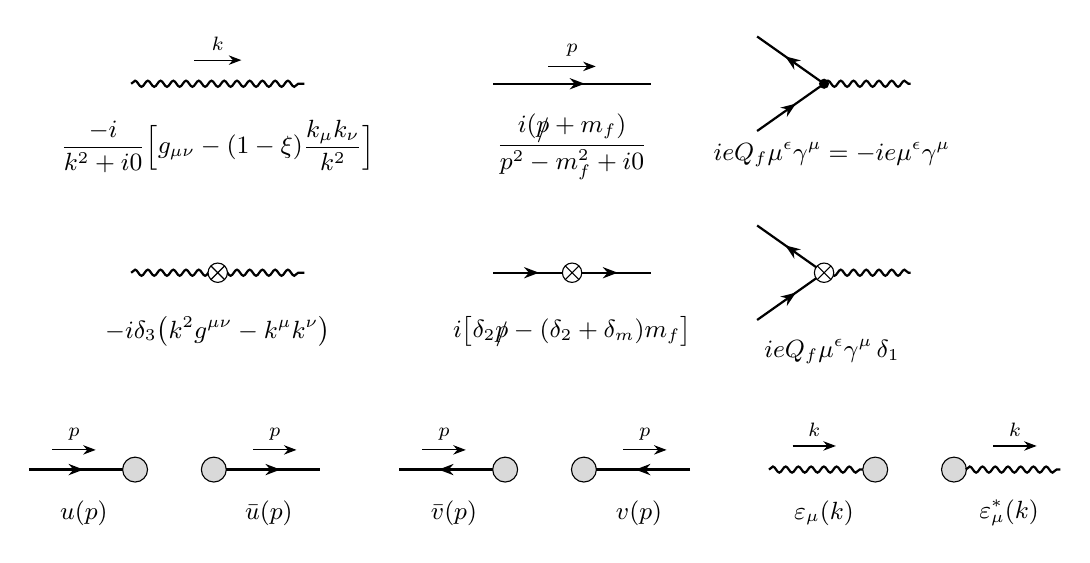
\begin{tikzpicture}
\begin{scope}[shift={(0,0)}]
  \draw[photon] (0,0) -- (2.2,0);
  \draw[mom] (0.8,0.3) -- (1.4,0.3) node[midway,above,font=\scriptsize] {$k$};
  \node[lab] at (1.1,-0.8) {$\dfrac{-i}{k^2+i0}\Bigl[g_{\mu\nu}-(1-\xi)\dfrac{k_\mu k_\nu}{k^2}\Bigr]$};
\end{scope}
\begin{scope}[shift={(4.6,0)}]
  \draw[fermion] (0,0) -- (2,0);
  \draw[mom] (0.7,0.22) -- (1.3,0.22) node[midway,above,font=\scriptsize] {$p$};
  \node[lab] at (1,-0.8) {$\dfrac{i(\slashed p+m_f)}{p^2-m_f^2+i0}$};
\end{scope}
\begin{scope}[shift={(8.8,0)}]
  \draw[fermion] (-0.85,-0.6) -- (0,0);
  \draw[fermion] (0,0) -- (-0.85,0.6);
  \draw[photon] (0,0) -- (1.1,0);
  \node[vtx] at (0,0) {};
  \node[lab] at (0.1,-0.9) {$ieQ_f\mu^{\epsilon}\gamma^\mu=-ie\mu^\epsilon\gamma^\mu$};
\end{scope}
\begin{scope}[shift={(0,-2.4)}]
  \draw[photon] (0,0) -- (2.2,0);
  \node[ctv] at (1.1,0) {};
  \node[lab] at (1.1,-0.75) {$-i\delta_3\bigl(k^2g^{\mu\nu}-k^\mu k^\nu\bigr)$};
\end{scope}
\begin{scope}[shift={(4.6,-2.4)}]
  \draw[fermion] (0,0) -- (1,0);
  \draw[fermion] (1,0) -- (2,0);
  \node[ctv] at (1,0) {};
  \node[lab] at (1,-0.75) {$i\bigl[\delta_2\slashed p-(\delta_2+\delta_m)m_f\bigr]$};
\end{scope}
\begin{scope}[shift={(8.8,-2.4)}]
  \draw[fermion] (-0.85,-0.6) -- (0,0);
  \draw[fermion] (0,0) -- (-0.85,0.6);
  \draw[photon] (0,0) -- (1.1,0);
  \node[ctv] at (0,0) {};
  \node[lab] at (0.1,-1.0) {$ieQ_f\mu^{\epsilon}\gamma^\mu\,\delta_1$};
\end{scope}
\begin{scope}[shift={(-1.3,-4.9)}]
  \draw[fermion] (0,0) -- (1.2,0); \node[blob] at (1.35,0) {};
  \draw[mom] (0.3,0.25) -- (0.85,0.25) node[midway,above,ml] {$p$};
  \node[lab] at (0.7,-0.55) {$u(p)$};
  \node[blob] at (2.35,0) {}; \draw[fermion] (2.5,0) -- (3.7,0);
  \draw[mom] (2.85,0.25) -- (3.4,0.25) node[midway,above,ml] {$p$};
  \node[lab] at (3.05,-0.55) {$\bar u(p)$};
  \draw[fermion] (5.9,0) -- (4.7,0); \node[blob] at (6.05,0) {};
  \draw[mom] (5.0,0.25) -- (5.55,0.25) node[midway,above,ml] {$p$};
  \node[lab] at (5.4,-0.55) {$\bar v(p)$};
  \node[blob] at (7.05,0) {}; \draw[fermion] (8.4,0) -- (7.2,0);
  \draw[mom] (7.55,0.25) -- (8.1,0.25) node[midway,above,ml] {$p$};
  \node[lab] at (7.75,-0.55) {$v(p)$};
  \draw[photon] (9.4,0) -- (10.6,0); \node[blob] at (10.75,0) {};
  \draw[mom] (9.7,0.3) -- (10.25,0.3) node[midway,above,ml] {$k$};
  \node[lab] at (10.1,-0.55) {$\varepsilon_\mu(k)$};
  \node[blob] at (11.75,0) {}; \draw[photon] (11.9,0) -- (13.1,0);
  \draw[mom] (12.25,0.3) -- (12.8,0.3) node[midway,above,ml] {$k$};
  \node[lab] at (12.45,-0.55) {$\varepsilon^*_\mu(k)$};
\end{scope}
\end{tikzpicture}
\caption{式~\eqref{eq:L} から導いた Feynman 則（\ref{app:rules}）。波線は光子、矢印の付いた実線はフェルミオン $f=e,\mu$ で、矢印はフェルミオン数の流れの向きである。上の段は左から光子とフェルミオンの伝播関数、頂点。中の段はそれぞれの対抗項で、$\otimes$ は対抗項の挿入を表す。下の段は外線の因子で、灰色の丸は図の残りの部分、細い矢印は運動量の向きである。左から、入ってくるフェルミオン $u(p)$、出ていくフェルミオン $\bar u(p)$、入ってくる反フェルミオン $\bar v(p)$、出ていく反フェルミオン $v(p)$、入ってくる光子 $\varepsilon_\mu(k)$、出ていく光子 $\varepsilon^*_\mu(k)$。反フェルミオンではフェルミオン数の矢印が運動量と逆を向く。ループ運動量ごとに $\int\dd^Dk/(2\pi)^D$ を掛ける。閉じたフェルミオンのループには $-1$ とトレースが付く。}
\label{fig:rules}
\end{figure}

\begin{figure}[tbp]
\centering
\begin{tikzpicture}
% (a) vacuum polarization
\begin{scope}[shift={(0,0)}]
  \draw[photon] (-1.6,0) -- (-0.55,0);
  \draw[photon] (0.55,0) -- (1.6,0);
  \draw[fermion] (0.55,0) arc (0:180:0.55);
  \draw[fermion] (-0.55,0) arc (180:360:0.55);
  \node[vtx] at (-0.55,0) {}; \node[vtx] at (0.55,0) {};
  \draw[mom] (-1.45,0.3) -- (-0.95,0.3) node[midway,above,ml] {$q$};
  \draw[mom] (0.95,0.3) -- (1.45,0.3) node[midway,above,ml] {$q$};
  \node[ml] at (0,0.78) {$k$}; \node[ml] at (0,-0.78) {$k+q$};
  \node[ml] at (-0.62,-0.27) {$\mu$}; \node[ml] at (0.62,-0.27) {$\nu$};
  \node[lab] at (0,-1.25) {(a) $\Pi_f$：$e^2$（$f=e,\mu$）};
  \node[lab,font=\footnotesize] at (0,-1.7) {$1$（$-1$ とトレース）};
\end{scope}
% (b) self-energy
\begin{scope}[shift={(4.6,-0.3)}]
  \draw[fermion] (-1.5,0) -- (-0.7,0);
  \draw[fermion] (-0.7,0) -- (0.7,0);
  \draw[fermion] (0.7,0) -- (1.5,0);
  \draw[photon] (0.7,0) arc (0:180:0.7);
  \node[vtx] at (-0.7,0) {}; \node[vtx] at (0.7,0) {};
  \draw[mom] (-1.45,-0.25) -- (-0.95,-0.25) node[midway,below,ml] {$p$};
  \draw[mom] (0.95,-0.25) -- (1.45,-0.25) node[midway,below,ml] {$p$};
  \node[ml] at (0,-0.22) {$k$}; \node[ml] at (0,0.95) {$q=p-k$};
  \node[lab] at (0,-0.95) {(b) $\Sigma_f$：$e^2$};
  \node[lab,font=\footnotesize] at (0,-1.4) {$1$};
\end{scope}
% (c) vertex
\begin{scope}[shift={(9.4,-0.3)}]
  \draw[fermion] (-1.75,0) -- (-0.9,0);
  \draw[fermion] (-0.9,0) -- (0,0);
  \draw[fermion] (0,0) -- (0.9,0);
  \draw[fermion] (0.9,0) -- (1.75,0);
  \draw[photon] (0.9,0) arc (0:180:0.9);
  \draw[photon] (0,0) -- (0,-0.85);
  \node[vtx] at (-0.9,0) {}; \node[vtx] at (0,0) {}; \node[vtx] at (0.9,0) {};
  \draw[mom] (-1.7,-0.25) -- (-1.2,-0.25) node[midway,below,ml] {$p$};
  \draw[mom] (1.2,-0.25) -- (1.7,-0.25) node[midway,below,ml] {$p'$};
  \node[ml] at (-0.47,-0.22) {$p-l$}; \node[ml] at (0.5,-0.22) {$p'-l$};
  \node[ml] at (0,1.12) {$l$}; \node[ml] at (0.3,-0.68) {$q,\mu$};
  \node[lab] at (0,-1.25) {(c) $\Lambda^\mu$：$e^2$};
  \node[lab,font=\footnotesize] at (0,-1.7) {$1$};
\end{scope}
% (d) photon 1-point
\begin{scope}[shift={(0,-3.6)}]
  \draw[photon] (-1.2,0) -- (0,0);
  \draw[fermion] (0,0) arc (-90:270:0.5);
  \node[vtx] at (0,0) {};
  \node[lab] at (0,-0.6) {(d) 光子1点};
  \node[lab,font=\footnotesize] at (0,-1.05) {奇関数の積分で $0$};
\end{scope}
% (e) photon 3-point
\begin{scope}[shift={(4.6,-3.4)}]
  \coordinate (A) at (-0.6,0); \coordinate (B) at (0.45,0.6); \coordinate (C) at (0.45,-0.6);
  \draw[fermion] (A) -- (B); \draw[fermion] (B) -- (C); \draw[fermion] (C) -- (A);
  \draw[photon] (A) -- (-1.4,0) (B) -- (1.05,1.1) (C) -- (1.05,-1.1);
  \node[vtx] at (A) {}; \node[vtx] at (B) {}; \node[vtx] at (C) {};
  \node[lab] at (0,-1.5) {(e) 光子3点（2通り）};
  \node[lab,font=\footnotesize] at (0,-1.95) {向きの逆な2つが打ち消す};
\end{scope}
% (f) photon 4-point
\begin{scope}[shift={(9.2,-3.4)}]
  \draw[fermion] (-0.55,-0.55) -- (0.55,-0.55);
  \draw[fermion] (0.55,-0.55) -- (0.55,0.55);
  \draw[fermion] (0.55,0.55) -- (-0.55,0.55);
  \draw[fermion] (-0.55,0.55) -- (-0.55,-0.55);
  \draw[photon] (-0.55,0.55) -- (-1.05,1.05) (0.55,0.55) -- (1.05,1.05) (-0.55,-0.55) -- (-1.05,-1.05) (0.55,-0.55) -- (1.05,-1.05);
  \node[vtx] at (-0.55,0.55) {}; \node[vtx] at (0.55,0.55) {}; \node[vtx] at (-0.55,-0.55) {}; \node[vtx] at (0.55,-0.55) {};
  \node[lab] at (0,-1.5) {(f) 光子4点（6通り）};
  \node[lab,font=\footnotesize] at (0,-1.95) {和は紫外で有限};
\end{scope}
\end{tikzpicture}
\caption{1ループの1PI 図（\ref{app:rules}）。(a)〜(c) には、\ref{app:ward}、\ref{app:ren} の式で使う運動量の割り当てを書いた（$p'=p+q$）。(a) と (d)〜(f) は閉じたフェルミオンのループで、フレーバー $e$、$\mu$ のそれぞれについて現れ、$-1$ とトレースが付く。対称性因子はすべて1である。(d) は被積分関数が奇関数になって0である。(e) の2通りは向きの逆なループで、Furry の定理により打ち消す。(f) の6通りは4本の外線をループに付ける巡回の順序（$3!=6$）で、一つ一つは対数発散するが和は有限である。}
\label{fig:oneloop}
\end{figure}

\paragraph{Furry の定理と消える図。}光子の1点関数 (d) は $\mathrm{tr}[\gamma^\mu(\slashed k+m)]=4k^\mu$ の積分で、被積分関数が $k$ の奇関数なので0である。光子の3点関数 (e) の2通りの図は、荷電共役 $C\gamma^\mu C^{-1}=-(\gamma^\mu)^T$ によって、一方のトレースが他方の $(-1)^3$ 倍になり、和が0になる（Furry の定理~\cite{furry}、\ref{app:rules}）。一般に、奇数本の光子をフェルミオンのループに付けた図の和は0である。

\paragraph{べき数え上げ。}外の光子線 $E_\gamma$ 本、外のフェルミオン線 $E_\psi$ 本の図の表面的な発散次数は、$d=4$ で
\begin{equation}
\omega=4-E_\gamma-\frac32E_\psi
\label{eq:omega}
\end{equation}
である（\ref{app:counting}）。$\omega\ge0$ となるのは $(E_\gamma,E_\psi)=(1,0),(2,0),(3,0),(4,0),(0,2),(1,2)$ の6種類である。$(1,0)$ と $(3,0)$ は上で述べたように0である。光子4点関数 $(4,0)$ は $\omega=0$ だが、ゲージ不変性により外線ごとに場の強さ $F_{\mu\nu}$、すなわち運動量が一つずつ付くので、実質の次数は $-4$ で有限である。光子2点関数 $(2,0)$ は $\omega=2$ だが、横波性（下の式~\eqref{eq:ward}）により $q^2$ が括り出されて対数発散になる。残りのフェルミオンの2点関数（$\omega=1$）と頂点（$\omega=0$）を合わせた三つが、式~\eqref{eq:L} の対抗項 $\delta_3$、$\delta_2$、$\delta_m$、$\delta_1$ に対応する。光子の質量項や $(A^2)^2$ の対抗項は要らない。

\begin{figure}[tbp]
\centering
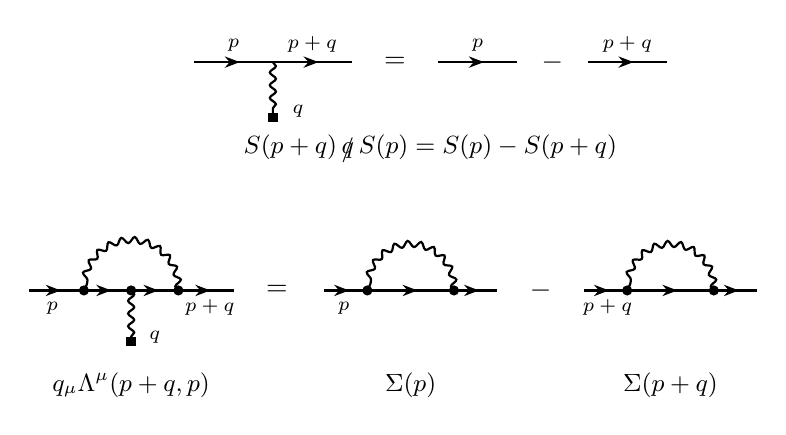
\begin{tikzpicture}
\begin{scope}[shift={(0,0)}]
  \draw[fermion] (0,0) -- (1,0); \draw[fermion] (1,0) -- (2,0);
  \draw[photon] (1,0) -- (1,-0.65); \node[qdot] at (1,-0.7) {};
  \node[ml] at (1.32,-0.62) {$q$};
  \node[ml] at (0.5,0.22) {$p$}; \node[ml] at (1.5,0.22) {$p+q$};
  \node at (2.55,0) {$=$};
  \draw[fermion] (3.1,0) -- (4.1,0); \node[ml] at (3.6,0.22) {$p$};
  \node at (4.55,0) {$-$};
  \draw[fermion] (5.0,0) -- (6.0,0); \node[ml] at (5.5,0.22) {$p+q$};
  \node[lab] at (3.0,-1.1) {$S(p+q)\,\slashed q\,S(p)=S(p)-S(p+q)$};
\end{scope}
\begin{scope}[shift={(-0.8,-2.9)}]
  \draw[fermion] (-1.3,0) -- (-0.6,0); \draw[fermion] (-0.6,0) -- (0,0);
  \draw[fermion] (0,0) -- (0.6,0); \draw[fermion] (0.6,0) -- (1.3,0);
  \draw[photon] (0.6,0) arc (0:180:0.6);
  \draw[photon] (0,0) -- (0,-0.6); \node[qdot] at (0,-0.65) {};
  \node[vtx] at (-0.6,0) {}; \node[vtx] at (0,0) {}; \node[vtx] at (0.6,0) {};
  \node[ml] at (0.3,-0.6) {$q$}; \node[ml] at (-1.0,-0.22) {$p$}; \node[ml] at (1.0,-0.22) {$p+q$};
  \node[lab] at (0,-1.2) {$q_\mu\Lambda^\mu(p+q,p)$};
  \node at (1.85,0) {$=$};
  \begin{scope}[shift={(3.55,0)}]
    \draw[fermion] (-1.1,0) -- (-0.55,0); \draw[fermion] (-0.55,0) -- (0.55,0); \draw[fermion] (0.55,0) -- (1.1,0);
    \draw[photon] (0.55,0) arc (0:180:0.55);
    \node[vtx] at (-0.55,0) {}; \node[vtx] at (0.55,0) {};
    \node[ml] at (-0.85,-0.22) {$p$};
    \node[lab] at (0,-1.2) {$\Sigma(p)$};
  \end{scope}
  \node at (5.2,0) {$-$};
  \begin{scope}[shift={(6.85,0)}]
    \draw[fermion] (-1.1,0) -- (-0.55,0); \draw[fermion] (-0.55,0) -- (0.55,0); \draw[fermion] (0.55,0) -- (1.1,0);
    \draw[photon] (0.55,0) arc (0:180:0.55);
    \node[vtx] at (-0.55,0) {}; \node[vtx] at (0.55,0) {};
    \node[ml] at (-0.8,-0.22) {$p+q$};
    \node[lab] at (0,-1.2) {$\Sigma(p+q)$};
  \end{scope}
\end{scope}
\end{tikzpicture}
\caption{Ward--Takahashi 恒等式~\eqref{eq:ward} を図で表したもの（\ref{app:ward}）。黒い四角は、光子の線を外して運動量 $q$ で縮約すること（$\gamma^\mu\to\slashed q$）を表す。上の段：縮約した頂点は、その両側のフェルミオンの伝播関数の差になる（運動量 $p+q$ の線が消えたものから、運動量 $p$ の線が消えたものを引く）。下の段：これを頂点の補正の中の頂点に使うと、ループの中の伝播関数が一つずつ消え、頂点の補正は二つの自己エネルギーの差になる。光子の伝播関数（$\xi$ を含む）は関与しないので、任意の $\xi$ で成り立つ。光子の2点関数では、同じ縮約が積分変数をずらした二つの同じ積分の差になって0になる（横波性）。}
\label{fig:ward}
\end{figure}

\paragraph{Ward--Takahashi 恒等式。}1ループで、任意の $\xi$ について
\begin{equation}
q_\mu\Pi^{\mu\nu}(q)=0,\qquad
q_\mu\Lambda^\mu(p+q,p)=\Sigma(p)-\Sigma(p+q),\qquad
\Lambda^\mu(p,p)=-\frac{\partial\Sigma(p)}{\partial p_\mu}
\label{eq:ward}
\end{equation}
が成り立つ（Ward~\cite{ward}、Takahashi~\cite{takahashi}、\ref{app:ward}）。図~\ref{fig:ward} がその仕組みで、光子の線を運動量で縮約するとフェルミオンの伝播関数が一つ消える。一つ目から $\Pi^{\mu\nu}=(q^2g^{\mu\nu}-q^\mu q^\nu)\Pi(q^2)$ となり、光子は質量を得ない。二つ目と三つ目から、頂点の発散と自己エネルギーの $\slashed p$ の発散が結びつき、$\delta_1^f=\delta_2^f$、したがって $Z_e=Z_3^{-1/2}$ となる。電荷の繰り込みは光子の場の繰り込みだけで決まり、$e$ と $\mu$ で共通である。

\paragraph{1ループの1PI 関数。}伝播関数の分母を $D_a(k)\equiv k^2-m_a^2+i0$ と書き、1点と2点のスカラー積分を
\begin{equation}
I_1^a\equiv\mu^{2\epsilon}\int\frac{\dd^Dk}{(2\pi)^D}\frac{1}{D_a(k)}=\frac iKA_0(m_a^2),\qquad
I_2^{ab}(p^2)\equiv\mu^{2\epsilon}\int\frac{\dd^Dk}{(2\pi)^D}\frac{1}{D_a(k)\,D_b(k+p)}=\frac iKB_0(p^2;m_a^2,m_b^2)
\label{eq:IN}
\end{equation}
と定義する（$K=(4\pi)^2$）。$B_1$ は $\mu^{2\epsilon}(K/i)\int\dd^Dk\,k^\mu/[(2\pi)^DD_a(k)D_b(k+p)]$ の $p^\mu$ の係数で、$p^2B_1=\frac12[A_0(m_a^2)-A_0(m_b^2)-(p^2+m_a^2-m_b^2)B_0]$ である。図~\ref{fig:oneloop} の (a)〜(c) を Feynman 則で書き、トレースと $D$ 次元の $\gamma$ 行列の縮約、部分積分の恒等式で整理すると、$D$ 次元で
\begin{equation}
\begin{aligned}
\Pi_f(q^2)&=\frac{e^2}{K}\,\frac{2}{(D-1)q^2}\Bigl[2(D-2)A_0(m_f^2)-\bigl(4m_f^2+(D-2)q^2\bigr)B_0(q^2;m_f^2,m_f^2)\Bigr],\\
\Sigma_f(p)&=\frac{e^2}{K}\Bigl[\xi(D-2)\,\slashed p\,B_1(p^2;m_f^2,0)+(D-1+\xi)\,m_f\,B_0(p^2;m_f^2,0)\Bigr],\\
F_1^\Lambda(q^2)&=\frac{e^2}{K}\Bigl\{\xi\DUV+(1-\xi)\DIR+(2m^2-q^2)\!\int_0^1\!\dd w\,\frac{\DIR-\ln(h(w)/\mu^2)}{h(w)}\\
&\hspace{3.2em}-2-\int_0^1\!\dd w\ln\frac{h(w)}{\mu^2}+2(3m^2-q^2)\int_0^1\frac{\dd w}{h(w)}\Bigr\},\\
F_2(q^2)&=\frac{2e^2m^2}{K}\int_0^1\frac{\dd w}{h(w)},\qquad h(w)\equiv m^2-q^2w(1-w)
\end{aligned}
\label{eq:V}
\end{equation}
となる（\ref{app:ren}）。$\Pi_f$ と $\Sigma_f$ は対抗項を含まない値で、$A_0$、$B_0$、$B_1$ は $D$ 次元の積分（極を含む）である。頂点は質量殻上（$p^2=p'^2=m^2$、$q=p'-p$）の値で、$\bar u(p')\Lambda^\mu u(p)=\bar u(p')[\gamma^\mu F_1^\Lambda+\frac{i\sigma^{\mu\nu}q_\nu}{2m}F_2]u(p)$ と書いた。$F_1^\Lambda$ と $F_2$ は、三つの Feynman パラメータのうち二つの積分を実行した形で、残った $w$ は光子から見た二つのフェルミオンの線の分け方である（\ref{app:ren}）。$q^2>0$ では $h$ に $-i0$ を付ける。

式~\eqref{eq:V} の要点は三つある。一つ目に、自己エネルギーのゲージ依存の部分は、$q=p-k$ として $\slashed q\,(\slashed k+m)\slashed q=(\slashed p-m)(\slashed k+m)(\slashed p-m)+(\text{伝播関数を消す項})$ と書き直すと、スケールのない積分を除いて $(\slashed p-m)X(\slashed p-m)$ の形になる。$X$ を部分積分の恒等式で $A_0$、$B_0$ に直すと、$D$ 次元で厳密に $-(1-\xi)[(D-2)\slashed pB_1+mB_0]$ となり、Feynman ゲージの部分と合わせて上の短い形になる。その結果、$\Sigma_V$ は $\xi$ に比例し、Landau ゲージ（$\xi=0$）では1ループの場の繰り込みが0である。二つ目に、質量殻上の頂点のゲージ依存の部分は、外線のスピノルの Dirac 方程式で伝播関数が消えて $\bar u\gamma^\mu u\int\dd^Dl/l^4$ になる。これはスケールのない積分で、次元正則化では0である。したがって、$F_1^\Lambda$ の $\xi$ 依存は $\xi\DUV+(1-\xi)\DIR$ という形でしか現れず、数値としては $\xi$ によらない。三つ目に、$F_1^\Lambda$ の赤外の極は Feynman パラメータの角 $z\to1$ から来て、係数は $(1-\xi)+(2m^2-q^2)\int\dd w/h$ である。$F_2$ は紫外でも赤外でも有限で、$\xi$ にも $\mu$ にもよらない。

\paragraph{$\MSbar$ の対抗項。}式~\eqref{eq:V} の紫外の極を取り出すと（\ref{app:ren}）、それを消す対抗項は
\begin{equation}
\begin{gathered}
\delta_3=-\frac{4e^2}{3K}N_f\,\DUV,\qquad
\delta_2^f=-\xi\,\frac{e^2}{K}\,\DUV,\qquad
\delta_m^f=-\frac{3e^2}{K}\,\DUV,\\
\delta_1^f=\delta_2^f,\qquad
\delta_e\equiv Z_e-1=-\frac{\delta_3}{2}=\frac{2e^2}{3K}N_f\,\DUV
\end{gathered}
\label{eq:ct}
\end{equation}
である。$\delta_3$ は二つのフレーバーのループの和で、$N_f=2$ を入れると $-8e^2\DUV/(3K)$ になる。$\delta_2$ と $\delta_1$ は $\xi$ に依存するが、$\delta_m$、$\delta_3$、$\delta_e$ は依存しない。$\delta_1=\delta_2$ は式~\eqref{eq:ward} から従い、頂点の極を直接計算しても同じになる（\ref{app:ren}）。

\paragraph{繰り込まれた1PI 関数。}式~\eqref{eq:ct} を加えて $\epsilon\to0$ とすると
\begin{equation}
\begin{aligned}
\Pi_f^{\mathrm R}(q^2)&=-\frac{4e^2}{3K}\Bigl[\Bigl(1+\frac{2m_f^2}{q^2}\Bigr)B_0(q^2;m_f^2,m_f^2)-\frac{2m_f^2}{q^2}B_0(0;m_f^2,m_f^2)-\frac13\Bigr],\\
\Sigma_V^{\mathrm R}(p^2)&=\xi\,\frac{e^2}{K}\bigl[1+2B_1(p^2;m_f^2,0)\bigr],\qquad
\Sigma_S^{\mathrm R}(p^2)=\frac{e^2}{K}\bigl[(3+\xi)B_0(p^2;m_f^2,0)-2\bigr],\\
F_1^{\mathrm R}(q^2)&=1+F_1^\Lambda(q^2)+\delta_1=1+\frac{e^2}{K}\Bigl\{(1-\xi)\DIR+(2m^2-q^2)\!\int_0^1\!\dd w\,\frac{\DIR-\ln(h/\mu^2)}{h}+\cdots\Bigr\}
\end{aligned}
\label{eq:VR}
\end{equation}
となる（\ref{app:ren}）。$A_0$、$B_0$、$B_1$ はここでは LoopTools の規約の $\MSbar$ の有限部分（$\DUV=0$ の値）で、$B_0(0;m^2,m^2)=-\ln(m^2/\mu^2)$ である。$-1/3$、$1$、$-2$ は、$D$ 次元の係数の $O(\epsilon)$ の部分が紫外の極に掛かって生じる有限の項である。$F_1^{\mathrm R}$ の「$\cdots$」は式~\eqref{eq:V} の有限の三つの項である。自己エネルギーは $\Sigma=\slashed p\,\Sigma_V+m\Sigma_S$、光子の2点関数は $\Pi^{\mathrm R}=\sum_f\Pi_f^{\mathrm R}$ である。

\paragraph{繰り込み群。}裸の量が $\mu$ によらないことから（\ref{app:rg}）
\begin{equation}
\beta_e=\frac{4N_f}{3}\frac{e^3}{K}=\frac{8e^3}{3K},\qquad
\gamma_m^f=-\frac{6e^2}{K}\,m_f,\qquad
\gamma_\psi=\xi\,\frac{e^2}{K},\qquad
\gamma_A=\frac{4N_f}{3}\frac{e^2}{K}=\frac{\beta_e}{e},\qquad
\mu\frac{\dd\xi}{\dd\mu}=-2\gamma_A\,\xi
\label{eq:rge}
\end{equation}
を得る。$\beta_e=e\gamma_A$ は $Z_e=Z_3^{-1/2}$ の言い換えである。$\MSbar$ は質量によらない処方なので、$\beta_e$ はどのスケールでも二つのフレーバーを数える。1ループの解は
\begin{equation}
\frac{1}{\alpha(\mu)}=\frac{1}{\alpha(\mu_0)}-\frac{2N_f}{3\pi}\ln\frac{\mu}{\mu_0},\qquad
\mu_{\mathrm L}=\mu_0\exp\frac{3\pi}{2N_f\alpha(\mu_0)},\qquad
m_f(\mu)=m_f(\mu_0)\Bigl[\frac{\alpha(\mu)}{\alpha(\mu_0)}\Bigr]^{-9/(4N_f)}
\label{eq:run}
\end{equation}
で、$\alpha$ は $\mu$ とともに増え、$\mu_{\mathrm L}$ で発散する（Landau 極）。基準点 $e(\mu_0=m_e)=1$（$\alpha^{-1}=4\pi$）では $\ln(\mu_{\mathrm L}/m_e)=3\pi^2=29.6$、$\mu_{\mathrm L}=7.2\times10^{12}\,m_e$ である。物理の $\alpha$ では指数が $3\pi/(4\alpha)\approx323$ で、Landau 極は実質的に無限遠にある。質量は $\alpha^{-9/8}$ に比例して減る。

\paragraph{on-shell の量への換算。}$\MSbar$ の量で書いた S 行列要素は、極質量、留数、Thomson 極限の電荷で書き直せる。1ループで
\begin{equation}
\begin{gathered}
m_{f,\mathrm p}=m_f(\mu)\Bigl[1+\frac{e^2}{K}\Bigl(4+3\ln\frac{\mu^2}{m_f^2}\Bigr)\Bigr],\qquad
R_f=1-\frac{e^2}{K}\Bigl[(3-\xi)\DIR+4+3\ln\frac{\mu^2}{m_f^2}\Bigr],\\
R_A=1+\Pi^{\mathrm R}(0)=1-\frac{4e^2}{3K}\sum_f\ln\frac{\mu^2}{m_f^2},\qquad
e^2(\mu)=e_{\mathrm{OS}}^2\Bigl[1+\frac{4e^2}{3K}\sum_f\ln\frac{\mu^2}{m_f^2}\Bigr]
\end{gathered}
\label{eq:os}
\end{equation}
である（\ref{app:os}）。極質量は $\xi$ によらない。$\Sigma_V$ と $\Sigma_S$ の $\xi$ 依存が $p^2=m^2$ で打ち消すからである。$\mu$ にもよらない（$\gamma_m^f$ と $\ln\mu^2$ の係数が打ち消す）。フェルミオンの留数 $R_f$ は $\xi$ に依存する赤外の極を持つ。これを正しく得るには、$\Sigma$ の微分を $D$ 次元で行い、$(D-2)B_1'$ と $(D-1+\xi)B_0'$ の $O(\epsilon)$ の部分が赤外の極に掛かる有限の項 $2(1-\xi)$ を残す必要がある（\ref{app:os}）。式~\eqref{eq:ward} から $R_fF_1^{\mathrm R}(0)=1$ が成り立つので、外線の光子の電荷は $e(\mu)R_A^{1/2}=e_{\mathrm{OS}}$ となり、$e_{\mathrm{OS}}$ は $\mu$ にも $\xi$ にもよらない。基準点では $m_{e,\mathrm p}=1.02533$、$m_{\mu,\mathrm p}=1.70879$、$e_{\mathrm{OS}}=1.00451$（$\alpha^{-1}(0)=12.454$、$\alpha^{-1}(\mu)=12.566$）である。

\begin{figure}[tbp]
\centering
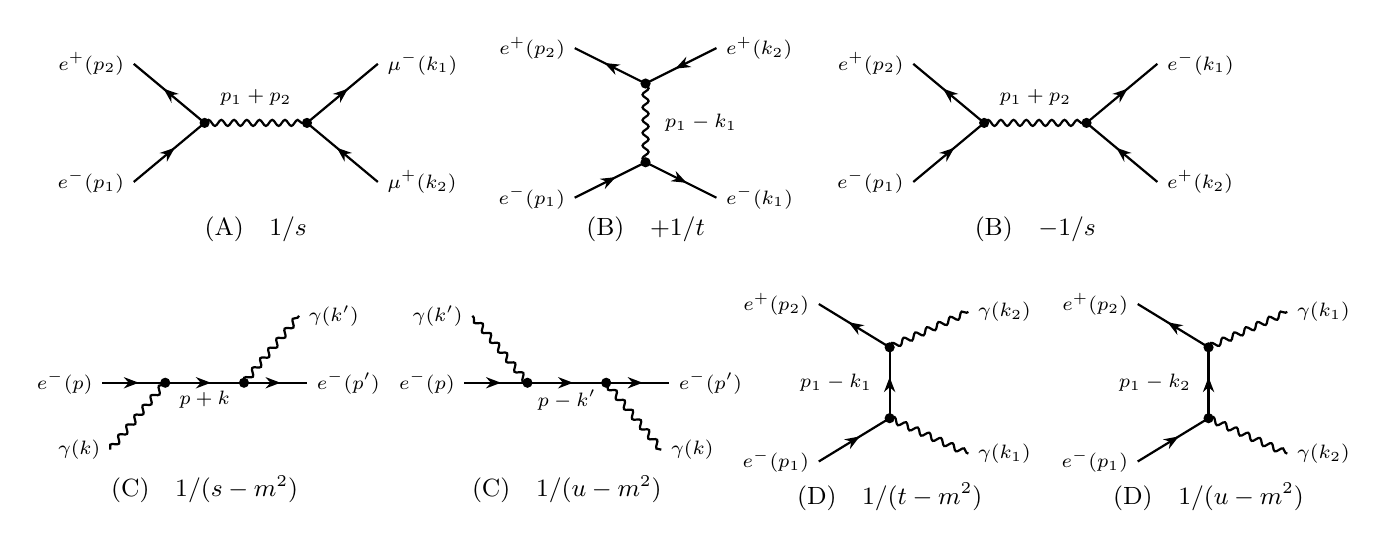
\begin{tikzpicture}
\begin{scope}[shift={(0,0)}]
  \draw[fermion] (-0.9,-0.75) -- (0,0); \draw[fermion] (0,0) -- (-0.9,0.75);
  \draw[photon] (0,0) -- (1.3,0);
  \draw[fermion] (1.3,0) -- (2.2,0.75); \draw[fermion] (2.2,-0.75) -- (1.3,0);
  \node[vtx] at (0,0) {}; \node[vtx] at (1.3,0) {};
  \node[ml,anchor=east] at (-0.9,-0.75) {$e^-(p_1)$}; \node[ml,anchor=east] at (-0.9,0.75) {$e^+(p_2)$};
  \node[ml,anchor=west] at (2.2,0.75) {$\mu^-(k_1)$}; \node[ml,anchor=west] at (2.2,-0.75) {$\mu^+(k_2)$};
  \node[ml] at (0.65,0.32) {$p_1+p_2$};
  \node[lab] at (0.65,-1.35) {(A)\quad $1/s$};
\end{scope}
\begin{scope}[shift={(5.6,0)}]
  \draw[fermion] (-0.9,-0.95) -- (0,-0.5); \draw[fermion] (0,-0.5) -- (0.9,-0.95);
  \draw[fermion] (0,0.5) -- (-0.9,0.95); \draw[fermion] (0.9,0.95) -- (0,0.5);
  \draw[photon] (0,-0.5) -- (0,0.5);
  \node[vtx] at (0,-0.5) {}; \node[vtx] at (0,0.5) {};
  \node[ml,anchor=east] at (-0.9,-0.95) {$e^-(p_1)$}; \node[ml,anchor=west] at (0.9,-0.95) {$e^-(k_1)$};
  \node[ml,anchor=east] at (-0.9,0.95) {$e^+(p_2)$}; \node[ml,anchor=west] at (0.9,0.95) {$e^+(k_2)$};
  \node[ml,anchor=west] at (0.12,0) {$p_1-k_1$};
  \node[lab] at (0,-1.35) {(B)\quad $+1/t$};
\end{scope}
\begin{scope}[shift={(9.9,0)}]
  \draw[fermion] (-0.9,-0.75) -- (0,0); \draw[fermion] (0,0) -- (-0.9,0.75);
  \draw[photon] (0,0) -- (1.3,0);
  \draw[fermion] (1.3,0) -- (2.2,0.75); \draw[fermion] (2.2,-0.75) -- (1.3,0);
  \node[vtx] at (0,0) {}; \node[vtx] at (1.3,0) {};
  \node[ml,anchor=east] at (-0.9,-0.75) {$e^-(p_1)$}; \node[ml,anchor=east] at (-0.9,0.75) {$e^+(p_2)$};
  \node[ml,anchor=west] at (2.2,0.75) {$e^-(k_1)$}; \node[ml,anchor=west] at (2.2,-0.75) {$e^+(k_2)$};
  \node[ml] at (0.65,0.32) {$p_1+p_2$};
  \node[lab] at (0.65,-1.35) {(B)\quad $-1/s$};
\end{scope}
\begin{scope}[shift={(0,-3.3)}]
  \draw[fermion] (-1.3,0) -- (-0.5,0); \draw[fermion] (-0.5,0) -- (0.5,0); \draw[fermion] (0.5,0) -- (1.3,0);
  \draw[photon] (-1.2,-0.85) -- (-0.5,0); \draw[photon] (0.5,0) -- (1.2,0.85);
  \node[vtx] at (-0.5,0) {}; \node[vtx] at (0.5,0) {};
  \node[ml,anchor=east] at (-1.3,0) {$e^-(p)$}; \node[ml,anchor=west] at (1.3,0) {$e^-(p')$};
  \node[ml,anchor=east] at (-1.2,-0.85) {$\gamma(k)$}; \node[ml,anchor=west] at (1.2,0.85) {$\gamma(k')$};
  \node[ml] at (0,-0.22) {$p+k$};
  \node[lab] at (0,-1.35) {(C)\quad $1/(s-m^2)$};
\end{scope}
\begin{scope}[shift={(4.6,-3.3)}]
  \draw[fermion] (-1.3,0) -- (-0.5,0); \draw[fermion] (-0.5,0) -- (0.5,0); \draw[fermion] (0.5,0) -- (1.3,0);
  \draw[photon] (-0.5,0) -- (-1.2,0.85); \draw[photon] (1.2,-0.85) -- (0.5,0);
  \node[vtx] at (-0.5,0) {}; \node[vtx] at (0.5,0) {};
  \node[ml,anchor=east] at (-1.3,0) {$e^-(p)$}; \node[ml,anchor=west] at (1.3,0) {$e^-(p')$};
  \node[ml,anchor=east] at (-1.2,0.85) {$\gamma(k')$}; \node[ml,anchor=west] at (1.2,-0.85) {$\gamma(k)$};
  \node[ml] at (0,-0.22) {$p-k'$};
  \node[lab] at (0,-1.35) {(C)\quad $1/(u-m^2)$};
\end{scope}
\begin{scope}[shift={(8.7,-3.3)}]
  \draw[fermion] (-0.9,-1.0) -- (0,-0.45); \draw[fermion] (0,-0.45) -- (0,0.45); \draw[fermion] (0,0.45) -- (-0.9,1.0);
  \draw[photon] (0,-0.45) -- (1.0,-0.9); \draw[photon] (0,0.45) -- (1.0,0.9);
  \node[vtx] at (0,-0.45) {}; \node[vtx] at (0,0.45) {};
  \node[ml,anchor=east] at (-0.9,-1.0) {$e^-(p_1)$}; \node[ml,anchor=east] at (-0.9,1.0) {$e^+(p_2)$};
  \node[ml,anchor=west] at (1.0,-0.9) {$\gamma(k_1)$}; \node[ml,anchor=west] at (1.0,0.9) {$\gamma(k_2)$};
  \node[ml,anchor=east] at (-0.1,0) {$p_1-k_1$};
  \node[lab] at (0,-1.45) {(D)\quad $1/(t-m^2)$};
\end{scope}
\begin{scope}[shift={(12.75,-3.3)}]
  \draw[fermion] (-0.9,-1.0) -- (0,-0.45); \draw[fermion] (0,-0.45) -- (0,0.45); \draw[fermion] (0,0.45) -- (-0.9,1.0);
  \draw[photon] (0,-0.45) -- (1.0,-0.9); \draw[photon] (0,0.45) -- (1.0,0.9);
  \node[vtx] at (0,-0.45) {}; \node[vtx] at (0,0.45) {};
  \node[ml,anchor=east] at (-0.9,-1.0) {$e^-(p_1)$}; \node[ml,anchor=east] at (-0.9,1.0) {$e^+(p_2)$};
  \node[ml,anchor=west] at (1.0,-0.9) {$\gamma(k_2)$}; \node[ml,anchor=west] at (1.0,0.9) {$\gamma(k_1)$};
  \node[ml,anchor=east] at (-0.1,0) {$p_1-k_2$};
  \node[lab] at (0,-1.45) {(D)\quad $1/(u-m^2)$};
\end{scope}
\end{tikzpicture}
\caption{式~\eqref{eq:Mtree} の木の図。上の段は (A) $e^+e^-\to\mu^+\mu^-$ と (B) Bhabha 散乱、下の段は (C) Compton 散乱と (D) $e^+e^-\to\gamma\gamma$ である。内線の脇の運動量は伝播関数の運動量で、下の式はその伝播関数の分母（(B) は二つの図の相対的な符号も）を表す。(B) の $s$ チャンネルの $-1$ は Fermi 統計から来る。(C) の右の図は、電子がまず $k'$ を放出してから $k$ を吸収する $u$ チャンネルで、(D) の二つの図は二つの光子を入れ替えたものである。}
\label{fig:tree}
\end{figure}

\paragraph{木の振幅とスピン和。}四つの過程の木の図（図~\ref{fig:tree}）を Feynman 則で書くと、振幅は
\begin{equation}
\begin{aligned}
\mathcal M_A&=\frac{e^2}{s}\,\bigl[\bar v(p_2)\gamma^\nu u(p_1)\bigr]\bigl[\bar u(k_1)\gamma_\nu v(k_2)\bigr],\\
\mathcal M_B&=e^2\Bigl\{\frac1t\bigl[\bar u(k_1)\gamma^\nu u(p_1)\bigr]\bigl[\bar v(p_2)\gamma_\nu v(k_2)\bigr]-\frac1s\bigl[\bar u(k_1)\gamma^\nu v(k_2)\bigr]\bigl[\bar v(p_2)\gamma_\nu u(p_1)\bigr]\Bigr\},\\
\mathcal M_C&=-e^2\,\varepsilon^*_\mu(k')\varepsilon_\nu(k)\,\bar u(p')\Bigl[\frac{\gamma^\mu(\slashed p+\slashed k+m)\gamma^\nu}{s-m^2}+\frac{\gamma^\nu(\slashed p-\slashed k'+m)\gamma^\mu}{u-m^2}\Bigr]u(p),\\
\mathcal M_D&=-e^2\,\varepsilon^*_\mu(k_1)\varepsilon^*_\nu(k_2)\,\bar v(p_2)\Bigl[\frac{\gamma^\nu(\slashed p_1-\slashed k_1+m)\gamma^\mu}{t-m^2}+\frac{\gamma^\mu(\slashed p_1-\slashed k_2+m)\gamma^\nu}{u-m^2}\Bigr]u(p_1)
\end{aligned}
\label{eq:Mtree}
\end{equation}
である（\ref{app:tree}）。(A) $e^-(p_1)e^+(p_2)\to\mu^-(k_1)\mu^+(k_2)$、(B) $e^-(p_1)e^+(p_2)\to e^-(k_1)e^+(k_2)$（Bhabha）、(D) $e^-(p_1)e^+(p_2)\to\gamma(k_1)\gamma(k_2)$ では $s=(p_1+p_2)^2$、$t=(p_1-k_1)^2$、$u=(p_1-k_2)^2$、(C) $e^-(p)\gamma(k)\to e^-(p')\gamma(k')$（Compton）では $s=(p+k)^2$、$u=(p-k')^2$ とした。(C) と (D) では $m=m_e$ である。(B) の二つの項の相対的な符号 $-1$ は Fermi 統計から来る。外線のスピンと偏極について和をとると
\begin{equation}
\begin{aligned}
\sum|\mathcal M_A|^2&=\frac{8e^4}{s^2}\Bigl[(t-m_e^2-m_\mu^2)^2+(u-m_e^2-m_\mu^2)^2+2s(m_e^2+m_\mu^2)\Bigr],\\
\sum|\mathcal M_B|^2&=8e^4\Bigl[\frac{(s-2m^2)^2+(u-2m^2)^2+4m^2t}{t^2}+\frac{(t-2m^2)^2+(u-2m^2)^2+4m^2s}{s^2}\\
&\hspace{4.2em}+\frac{2(u-2m^2)(u-6m^2)}{st}\Bigr],\\
\sum|\mathcal M_C|^2&=8e^4\Bigl[-\frac{u-m^2}{s-m^2}-\frac{s-m^2}{u-m^2}+4m^2\Bigl(\frac{1}{s-m^2}+\frac{1}{u-m^2}\Bigr)\\
&\hspace{4.2em}+4m^4\Bigl(\frac{1}{s-m^2}+\frac{1}{u-m^2}\Bigr)^2\Bigr],\\
\sum|\mathcal M_D|^2&=8e^4\Bigl[\frac{u-m^2}{t-m^2}+\frac{t-m^2}{u-m^2}-4m^2\Bigl(\frac{1}{t-m^2}+\frac{1}{u-m^2}\Bigr)\\
&\hspace{4.2em}-4m^4\Bigl(\frac{1}{t-m^2}+\frac{1}{u-m^2}\Bigr)^2\Bigr]
\end{aligned}
\label{eq:sumtree}
\end{equation}
となる（\ref{app:tree}）。光子の偏極の和は $-g_{\mu\nu}$ で置き換えた。これが許されるのは、外線の光子の運動量で偏極を置き換えると振幅が0になる（Ward 恒等式）からである。(D) は (C) の交差 $s\to t$ に、フェルミオンを一つ交差させる符号 $-1$ を掛けたものである。(A) は閾値 $s\to4m_\mu^2$ で s 波から始まり、$\sigma\propto\beta_\mu(3-\beta_\mu^2)/2$（$\beta_\mu=\sqrt{1-4m_\mu^2/s}$）である。(C) は低エネルギーで Thomson の断面積 $8\pi\alpha^2/(3m^2)$ に近づく。

\begin{figure}[tbp]
\centering
\begin{tikzpicture}
% (i) vacuum polarization
\begin{scope}[shift={(0,0)}]
  \draw[fermion] (-0.95,-0.8) -- (0,0); \draw[fermion] (0,0) -- (-0.95,0.8);
  \draw[fermion] (1.6,0) -- (2.55,0.8); \draw[fermion] (2.55,-0.8) -- (1.6,0);
  \draw[photon] (0,0) -- (0.45,0); \draw[photon] (1.15,0) -- (1.6,0);
  \draw[fermion] (1.15,0) arc (0:180:0.35); \draw[fermion] (0.45,0) arc (180:360:0.35);
  \node[vtx] at (0,0) {}; \node[vtx] at (1.6,0) {}; \node[vtx] at (0.45,0) {}; \node[vtx] at (1.15,0) {};
  \node[ml,anchor=east] at (-0.95,-0.8) {$e^-$}; \node[ml,anchor=east] at (-0.95,0.8) {$e^+$};
  \node[ml,anchor=west] at (2.55,0.8) {$\mu^-$}; \node[ml,anchor=west] at (2.55,-0.8) {$\mu^+$};
  \node[ml] at (0.8,-0.55) {$f=e,\mu$};
  \node[lab] at (0.8,-1.3) {(i) 真空偏極 $\Pi_f(s)$};
\end{scope}
% (ii) vertex at the electron side
\begin{scope}[shift={(5.0,0)}]
  \draw[fermion] (-0.95,-0.8) -- (-0.5,-0.42); \draw[fermion] (-0.5,-0.42) -- (0,0);
  \draw[fermion] (0,0) -- (-0.5,0.42); \draw[fermion] (-0.5,0.42) -- (-0.95,0.8);
  \draw[photon] (-0.5,-0.42) -- (-0.5,0.42);
  \draw[photon] (0,0) -- (1.6,0);
  \draw[fermion] (1.6,0) -- (2.55,0.8); \draw[fermion] (2.55,-0.8) -- (1.6,0);
  \node[vtx] at (0,0) {}; \node[vtx] at (1.6,0) {}; \node[vtx] at (-0.5,-0.42) {}; \node[vtx] at (-0.5,0.42) {};
  \node[ml,anchor=east] at (-0.95,-0.8) {$e^-$}; \node[ml,anchor=east] at (-0.95,0.8) {$e^+$};
  \node[ml,anchor=west] at (2.55,0.8) {$\mu^-$}; \node[ml,anchor=west] at (2.55,-0.8) {$\mu^+$};
  \node[lab] at (0.8,-1.3) {(ii) 頂点の補正 $\Lambda_e$};
\end{scope}
% (iii) vertex at the muon side
\begin{scope}[shift={(10.0,0)}]
  \draw[fermion] (-0.95,-0.8) -- (0,0); \draw[fermion] (0,0) -- (-0.95,0.8);
  \draw[photon] (0,0) -- (1.6,0);
  \draw[fermion] (1.6,0) -- (2.1,0.42); \draw[fermion] (2.1,0.42) -- (2.55,0.8);
  \draw[fermion] (2.55,-0.8) -- (2.1,-0.42); \draw[fermion] (2.1,-0.42) -- (1.6,0);
  \draw[photon] (2.1,-0.42) -- (2.1,0.42);
  \node[vtx] at (0,0) {}; \node[vtx] at (1.6,0) {}; \node[vtx] at (2.1,-0.42) {}; \node[vtx] at (2.1,0.42) {};
  \node[ml,anchor=east] at (-0.95,-0.8) {$e^-$}; \node[ml,anchor=east] at (-0.95,0.8) {$e^+$};
  \node[ml,anchor=west] at (2.55,0.8) {$\mu^-$}; \node[ml,anchor=west] at (2.55,-0.8) {$\mu^+$};
  \node[lab] at (0.8,-1.3) {(iii) 頂点の補正 $\Lambda_\mu$};
\end{scope}
% (iv) direct box
\begin{scope}[shift={(0.1,-3.2)}]
  \draw[fermion] (-0.8,-1.0) -- (0,-0.5); \draw[fermion] (0,-0.5) -- (0,0.5); \draw[fermion] (0,0.5) -- (-0.8,1.0);
  \draw[fermion] (2.2,-1.0) -- (1.4,-0.5); \draw[fermion] (1.4,-0.5) -- (1.4,0.5); \draw[fermion] (1.4,0.5) -- (2.2,1.0);
  \draw[photon] (0,-0.5) -- (1.4,-0.5); \draw[photon] (0,0.5) -- (1.4,0.5);
  \node[vtx] at (0,-0.5) {}; \node[vtx] at (0,0.5) {}; \node[vtx] at (1.4,-0.5) {}; \node[vtx] at (1.4,0.5) {};
  \node[ml,anchor=east] at (-0.8,-1.0) {$e^-$}; \node[ml,anchor=east] at (-0.8,1.0) {$e^+$};
  \node[ml,anchor=west] at (2.2,1.0) {$\mu^-$}; \node[ml,anchor=west] at (2.2,-1.0) {$\mu^+$};
  \node[lab] at (0.7,-1.45) {(iv) 直接の箱};
\end{scope}
% (v) crossed box
\begin{scope}[shift={(5.1,-3.2)}]
  \draw[fermion] (-0.8,-1.0) -- (0,-0.5); \draw[fermion] (0,-0.5) -- (0,0.5); \draw[fermion] (0,0.5) -- (-0.8,1.0);
  \draw[fermion] (2.2,-1.0) -- (1.4,-0.5); \draw[fermion] (1.4,-0.5) -- (1.4,0.5); \draw[fermion] (1.4,0.5) -- (2.2,1.0);
  \draw[photon] (0,-0.5) -- (1.4,0.5); \draw[photon] (0,0.5) -- (1.4,-0.5);
  \node[vtx] at (0,-0.5) {}; \node[vtx] at (0,0.5) {}; \node[vtx] at (1.4,-0.5) {}; \node[vtx] at (1.4,0.5) {};
  \node[ml,anchor=east] at (-0.8,-1.0) {$e^-$}; \node[ml,anchor=east] at (-0.8,1.0) {$e^+$};
  \node[ml,anchor=west] at (2.2,1.0) {$\mu^-$}; \node[ml,anchor=west] at (2.2,-1.0) {$\mu^+$};
  \node[lab] at (0.7,-1.45) {(v) 交差した箱};
\end{scope}
% (vi) external leg
\begin{scope}[shift={(10.0,-3.2)}]
  \draw[fermion] (-1.3,-1.095) -- (-1.0,-0.842); \draw[fermion] (-1.0,-0.842) -- (-0.45,-0.379); \draw[fermion] (-0.45,-0.379) -- (0,0);
  \draw[fermion] (0,0) -- (-0.95,0.8);
  \draw[photon] (-0.45,-0.379) arc (40:220:0.36);
  \draw[photon] (0,0) -- (1.6,0);
  \draw[fermion] (1.6,0) -- (2.55,0.8); \draw[fermion] (2.55,-0.8) -- (1.6,0);
  \node[vtx] at (0,0) {}; \node[vtx] at (1.6,0) {}; \node[vtx] at (-1.0,-0.842) {}; \node[vtx] at (-0.45,-0.379) {};
  \node[ml,anchor=east] at (-1.3,-1.095) {$e^-$}; \node[ml,anchor=east] at (-0.95,0.8) {$e^+$};
  \node[ml,anchor=west] at (2.55,0.8) {$\mu^-$}; \node[ml,anchor=west] at (2.55,-0.8) {$\mu^+$};
  \node[lab] at (0.8,-1.55) {(vi) 外線の自己エネルギー};
\end{scope}
% (vii) counterterms
\begin{scope}[shift={(0,-6.3)}]
  \draw[fermion] (-0.95,-0.8) -- (0,0); \draw[fermion] (0,0) -- (-0.95,0.8);
  \draw[fermion] (1.6,0) -- (2.55,0.8); \draw[fermion] (2.55,-0.8) -- (1.6,0);
  \draw[photon] (0,0) -- (1.6,0); \node[ctv] at (0.8,0) {};
  \node[vtx] at (0,0) {}; \node[vtx] at (1.6,0) {};
  \node[ml,anchor=east] at (-0.95,-0.8) {$e^-$}; \node[ml,anchor=east] at (-0.95,0.8) {$e^+$};
  \node[ml,anchor=west] at (2.55,0.8) {$\mu^-$}; \node[ml,anchor=west] at (2.55,-0.8) {$\mu^+$};
  \node[lab] at (0.8,-1.3) {(vii) 対抗項 $\delta_3$};
\end{scope}
\begin{scope}[shift={(5.0,-6.3)}]
  \draw[fermion] (-0.95,-0.8) -- (0,0); \draw[fermion] (0,0) -- (-0.95,0.8);
  \draw[fermion] (1.6,0) -- (2.55,0.8); \draw[fermion] (2.55,-0.8) -- (1.6,0);
  \draw[photon] (0,0) -- (1.6,0); \node[ctv] at (0,0) {}; \node[vtx] at (1.6,0) {};
  \node[ml,anchor=east] at (-0.95,-0.8) {$e^-$}; \node[ml,anchor=east] at (-0.95,0.8) {$e^+$};
  \node[ml,anchor=west] at (2.55,0.8) {$\mu^-$}; \node[ml,anchor=west] at (2.55,-0.8) {$\mu^+$};
  \node[lab] at (0.8,-1.3) {対抗項 $\delta_1^e$};
\end{scope}
\begin{scope}[shift={(10.0,-6.3)}]
  \draw[fermion] (-0.95,-0.8) -- (0,0); \draw[fermion] (0,0) -- (-0.95,0.8);
  \draw[fermion] (1.6,0) -- (2.55,0.8); \draw[fermion] (2.55,-0.8) -- (1.6,0);
  \draw[photon] (0,0) -- (1.6,0); \node[vtx] at (0,0) {}; \node[ctv] at (1.6,0) {};
  \node[ml,anchor=east] at (-0.95,-0.8) {$e^-$}; \node[ml,anchor=east] at (-0.95,0.8) {$e^+$};
  \node[ml,anchor=west] at (2.55,0.8) {$\mu^-$}; \node[ml,anchor=west] at (2.55,-0.8) {$\mu^+$};
  \node[lab] at (0.8,-1.3) {対抗項 $\delta_1^\mu$};
\end{scope}
% (viii) real emission
\begin{scope}[shift={(0.2,-9.3)},scale=0.85]
  \draw[fermion] (-0.95,-0.8) -- (-0.5,-0.42); \draw[fermion] (-0.5,-0.42) -- (0,0); \draw[fermion] (0,0) -- (-0.95,0.8);
  \draw[photon] (-0.5,-0.42) -- (-0.25,-1.05);
  \draw[photon] (0,0) -- (1.6,0); \draw[fermion] (1.6,0) -- (2.55,0.8); \draw[fermion] (2.55,-0.8) -- (1.6,0);
  \node[vtx] at (0,0) {}; \node[vtx] at (1.6,0) {}; \node[vtx] at (-0.5,-0.42) {};
  \node[ml] at (0.0,-1.1) {$\gamma$};
\end{scope}
\begin{scope}[shift={(3.9,-9.3)},scale=0.85]
  \draw[fermion] (-0.95,-0.8) -- (0,0); \draw[fermion] (0,0) -- (-0.5,0.42); \draw[fermion] (-0.5,0.42) -- (-0.95,0.8);
  \draw[photon] (-0.5,0.42) -- (-0.25,1.05);
  \draw[photon] (0,0) -- (1.6,0); \draw[fermion] (1.6,0) -- (2.55,0.8); \draw[fermion] (2.55,-0.8) -- (1.6,0);
  \node[vtx] at (0,0) {}; \node[vtx] at (1.6,0) {}; \node[vtx] at (-0.5,0.42) {};
  \node[ml] at (0.0,1.1) {$\gamma$};
\end{scope}
\begin{scope}[shift={(7.6,-9.3)},scale=0.85]
  \draw[fermion] (-0.95,-0.8) -- (0,0); \draw[fermion] (0,0) -- (-0.95,0.8);
  \draw[photon] (0,0) -- (1.6,0);
  \draw[fermion] (1.6,0) -- (2.1,0.42); \draw[fermion] (2.1,0.42) -- (2.55,0.8); \draw[fermion] (2.55,-0.8) -- (1.6,0);
  \draw[photon] (2.1,0.42) -- (1.85,1.05);
  \node[vtx] at (0,0) {}; \node[vtx] at (1.6,0) {}; \node[vtx] at (2.1,0.42) {};
  \node[ml] at (1.6,1.1) {$\gamma$};
\end{scope}
\begin{scope}[shift={(11.3,-9.3)},scale=0.85]
  \draw[fermion] (-0.95,-0.8) -- (0,0); \draw[fermion] (0,0) -- (-0.95,0.8);
  \draw[photon] (0,0) -- (1.6,0);
  \draw[fermion] (1.6,0) -- (2.55,0.8); \draw[fermion] (2.55,-0.8) -- (2.1,-0.42); \draw[fermion] (2.1,-0.42) -- (1.6,0);
  \draw[photon] (2.1,-0.42) -- (1.85,-1.05);
  \node[vtx] at (0,0) {}; \node[vtx] at (1.6,0) {}; \node[vtx] at (2.1,-0.42) {};
  \node[ml] at (1.6,-1.1) {$\gamma$};
\end{scope}
\node[lab] at (6.6,-10.65) {(viii) 実の光子の放射 $e^+e^-\to\mu^+\mu^-\gamma$（$e^-$、$e^+$、$\mu^-$、$\mu^+$ からの放射）};
\end{tikzpicture}
\caption{$e^+e^-\to\mu^+\mu^-$ の $e^4$ の次数の補正（\ref{app:scat}）。(i) $s$ チャンネルの光子への真空偏極の挿入（ループは $e$ と $\mu$ の2通り）。(ii)、(iii) 電子側と $\mu$ 粒子側の頂点の補正。(iv)、(v) 二つの光子の交換（直接と交差の箱）。(vi) 外線の自己エネルギー。切断された振幅には入れず、LSZ の留数 $R_f$ として外線ごとに $R_f^{1/2}$ を掛ける（4本の外線のそれぞれ）。(vii) $\MSbar$ の対抗項の挿入。(i)〜(iii)、(vi)、(vii) を合わせたものが式~\eqref{eq:Ms} で、(iv)、(v) は式~\eqref{eq:Wbox} の $W_{\mathrm{box}}$ である。(viii) 同じ次数の断面積に寄与する実の光子の放射（$\mathcal M_A$ に $e$ が一つ増えた図）。その軟光子の領域の赤外の極が、(ii)〜(v) の赤外の極と打ち消す。}
\label{fig:eemumu}
\end{figure}

\paragraph{1ループの $e^+e^-\to\mu^+\mu^-$。}$e^4$ の次数の補正は、図~\ref{fig:eemumu} の (i)〜(v)、すなわち$s$ チャンネルの光子の真空偏極、二つの頂点の補正、外線の留数、二つの光子の交換（直接と交差の箱）からなる。前の三つは
\begin{equation}
\mathcal M_s^{(1)}+\mathcal M_A=\frac{e_{\mathrm{OS}}^2}{s}\bigl[1+\hat\Pi(s)\bigr]\,\bigl[\bar v(p_2)\Gamma_e^\nu u(p_1)\bigr]\bigl[\bar u(k_1)\Gamma_{\mu,\nu}v(k_2)\bigr],\qquad
\Gamma_f^\nu=\gamma^\nu\hat F_1^f(s)+\frac{i\sigma^{\nu\rho}q_\rho}{2m_f}F_2^f(s)
\label{eq:Ms}
\end{equation}
にまとまる（\ref{app:scat}）。ここで $\hat\Pi(s)=\sum_f[\Pi_f(s)-\Pi_f(0)]$、$\hat F_1(s)=1+F_1^\Lambda(s)-F_1^\Lambda(0)$ で、$q$ は各頂点に光子から流れ込む運動量である。式~\eqref{eq:Ms} は、$\MSbar$ の $e(\mu)$ と留数 $R_f$、$R_A$ で計算しても、Ward 恒等式 $R_fF_1^{\mathrm R}(0)=1$ と式~\eqref{eq:os} を使うと、$\alpha(0)$ と処方によらない量だけで書けることを表す。$\hat\Pi$ と $\hat F_1$ は紫外で有限で、$\xi$ にも $\mu$ にもよらない。$\hat F_1$ には赤外の極が残り、
\begin{equation}
\hat F_1(q^2)\big|_{\mathrm{IR}}=\frac{2e^2}{K}\,f_{\mathrm{IR}}(q^2)\,\DIR,\qquad
f_{\mathrm{IR}}(q^2)=\int_0^1\dd w\,\frac{m^2-q^2/2}{m^2-q^2w(1-w)}-1
\label{eq:fir}
\end{equation}
である（\ref{app:scat}）。$f_{\mathrm{IR}}(0)=0$ で、$-q^2\gg m^2$ では $f_{\mathrm{IR}}\to\ln(-q^2/m^2)-1$ と大きくなる。この極は、箱の図の赤外の極とともに、軟光子の放射 $e^+e^-\to\mu^+\mu^-\gamma$ の極と打ち消す（Bloch--Nordsieck~\cite{bn}）。箱の図は次に述べる。

\paragraph{木との干渉。}$\alpha^3$ の次数の断面積に入るのは、木の振幅と1ループの振幅の干渉 $W\equiv\sum\mathcal M_A^*\mathcal M^{(1)}$（外線のスピンについての和）である。以下、$m=m_e$、$M=m_\mu$、$\Sigma_m=m^2+M^2$、$\tau\equiv\Sigma_m-t=2p_1\cdot k_1$ と書き、スピン和も $D$ 次元でとる（CDR）。木のスピン和は
\begin{equation*}
B(D)\equiv\sum|\mathcal M_A|^2=\frac{4e^4}{s^2}\bigl[(D-2)s^2+4s\Sigma_m-4s\tau+4\tau^2\bigr]=B(4)-8\epsilon e^4
\end{equation*}
で、$B(4)$ は式~\eqref{eq:sumtree} の1行目である。干渉は
\begin{equation}
\begin{gathered}
W=B(D)\Bigl[\Pi^{\mathrm R}(s)+\sum_f\bigl(\hat F_1^f(s)-1\bigr)\Bigr]+F_2^e(s)\,Z_e+F_2^\mu(s)\,Z_\mu+W_{\mathrm{box}},\\
Z_e=\frac{4e^4}{s}\bigl[(D-2)s+4M^2\bigr],\qquad Z_\mu=\frac{4e^4}{s}\bigl[(D-2)s+4m^2\bigr],\qquad
W_{\mathrm{box}}=\frac{e^6}{Ks}\bigl[\mathcal N(s,t)-\mathcal N(s,u)\bigr]
\end{gathered}
\label{eq:Wbox}
\end{equation}
となる（\ref{app:scat}）。1行目の前の三つの項は式~\eqref{eq:Ms} を $\MSbar$ の $e(\mu)$ で書いたものの干渉で、$Z_f$ は $F_2$ の項のスピン和である。$\mathcal N(s,t)$ は直接の箱 (iv) の干渉を積分したもので、交差した箱 (v) の干渉は $-\mathcal N(s,u)$ である。

\paragraph{箱の図。}直接の箱の分母を $D_0=l^2$、$D_1=(l-p_1)^2-m^2$、$D_2=(l-k_1)^2-M^2$、$D_3=(l-p_1-p_2)^2$ とすると、スピン和をとった分子は $2l\cdot p_1=D_0-D_1$、$2l\cdot k_1=D_0-D_2$、$2l\cdot p_2=D_1-D_3+s$ によって $D_i$ の2次の多項式になる。その係数 $c_k(D)$ と、各項が分母を約して与える1ループ積分 $I_k$（LoopTools の規約）を表~\ref{tab:box} に示す。$\mathcal N(s,t)=4\sum_kc_k(D)\,I_k$ である（\ref{app:scat}）。交差した箱が直接の箱の $t\leftrightarrow u$ の $-1$ 倍になるのは、$\mu$ の線を荷電共役で裏返すと、光子の付く順序が直接の箱と同じになり、符号 $-1$ が出るからである。したがって $W_{\mathrm{box}}$ は $t\leftrightarrow u$ で符号を変える。$B(D)$ と $Z_f$ は $t\leftrightarrow u$ で対称なので、この次数の前後の非対称度は、仮想の補正では箱の図だけから来る。それぞれの箱は $\xi$ に依存するが、その部分は $B(D)$ に比例し、二つの箱の和で打ち消す。箱の図は紫外で有限である。

\begin{table}[tbp]
\centering\small
\caption{直接の箱と木の干渉の分子 $N_A=4\sum_kc_k(D)\,m_k$ の係数と、各単項式 $m_k$ を $D_0D_1D_2D_3$ で割って積分したもの $I_k$（LoopTools の規約 $(K/i)\mu^{2\epsilon}\int\dd^Dl/(2\pi)^D$、\ref{app:scat}）。$d_i\equiv D_i$、$\tau=\Sigma_m-t$、$\Sigma_m=m^2+M^2$。積分の引数は $B_0(p^2;m_0^2,m_1^2)$、$C(p_1^2,p_2^2,(p_1+p_2)^2;m_0^2,m_1^2,m_2^2)$、$D_0(p_1^2,p_2^2,p_3^2,p_4^2,(p_1+p_2)^2,(p_2+p_3)^2;m_0^2,\dots,m_3^2)$ の順で、$C_{1,2}^{(i)}$ は $d_i$ の行の $C_0$ と同じ引数のテンソル係数である。}
\label{tab:box}
\begin{tabularx}{\linewidth}{>{$}l<{$}>{\raggedright\arraybackslash$}p{6.3cm}<{$}>{\raggedright\arraybackslash$}X<{$}}
\toprule
m_k & c_k(D) & I_k \\
\midrule
1 & 4\tau(\Sigma_ms-s^2-s\tau+2\tau^2)+\frac32Ds^2\tau & D_0(m^2,m^2,M^2,M^2,s,t;0,m^2,0,M^2) \\
d_0 & 4\tau(\Sigma_m+s-\tau)-Ds\tau & C_0(m^2,M^2,t;m^2,0,M^2) \\
d_3 & 4\tau(\Sigma_m+s-\tau)-Ds\tau & C_0(m^2,t,M^2;0,m^2,M^2) \\
d_1 & 2(2\Sigma_ms-2s^2-4M^2\tau-3s\tau+4\tau^2)+\frac D2s(3s+2\tau) & C_0(M^2,M^2,s;0,M^2,0) \\
d_2 & 2(2\Sigma_ms-2s^2-4m^2\tau-3s\tau+4\tau^2)+\frac D2s(3s+2\tau) & C_0(m^2,m^2,s;0,m^2,0) \\
d_0^2 & (\frac32D-4)\tau & B_0(M^2;M^2,0)+2m^2C_0^{(0)}-(s-2m^2)C_1^{(0)}-(M^2-m^2-t)C_2^{(0)} \\
d_3^2 & (\frac32D-4)\tau & B_0(t;m^2,M^2)+s\bigl(C_0^{(3)}+C_1^{(3)}+C_2^{(3)}\bigr) \\
d_1^2 & (D-2)s & B_0(M^2;M^2,0)+\tau C_1^{(1)}+sC_2^{(1)} \\
d_2^2 & (D-2)s & B_0(m^2;m^2,0)+\tau C_1^{(2)}+sC_2^{(2)} \\
d_0d_1 & 2(2s+\tau)-\frac D2(3s+2\tau) & B_0(M^2;M^2,0) \\
d_0d_2 & 2(2s+\tau)-\frac D2(3s+2\tau) & B_0(m^2;m^2,0) \\
d_1d_3 & 2(2s+\tau)-\frac D2(3s+2\tau) & B_0(M^2;0,M^2) \\
d_2d_3 & 2(2s+\tau)-\frac D2(3s+2\tau) & B_0(m^2;0,m^2) \\
d_0d_3 & -4(2s-\tau)+D(3s-\tau) & B_0(t;m^2,M^2) \\
d_1d_2 & -4(s+\tau)+D(s+2\tau) & B_0(s;0,0) \\
\bottomrule
\end{tabularx}
\end{table}

\paragraph{赤外の極。}干渉の赤外の極は、軟光子の領域から
\begin{equation}
\begin{gathered}
W\big|_{\mathrm{IR}}=\frac{2e^2}{K}\,\DIR\,B(D)\bigl[f_{\mathrm{IR}}(s;m)+f_{\mathrm{IR}}(s;M)+G(t)-G(u)\bigr],\\
G(x)=(\Sigma_m-x)\int_0^1\frac{\dd w}{wm^2+(1-w)M^2-xw(1-w)}
\end{gathered}
\label{eq:Wir}
\end{equation}
である（\ref{app:scat}）。$f_{\mathrm{IR}}(s;m)$ は式~\eqref{eq:fir} の $f_{\mathrm{IR}}$ を質量 $m$ で $q^2=s+i0$ に解析接続したもので、$s>4m^2$ では $\beta=\sqrt{1-4m^2/s}$ として $f_{\mathrm{IR}}(s;m)=\frac{s-2m^2}{s\beta}\bigl[\ln\frac{1+\beta}{1-\beta}-i\pi\bigr]-1$ である。この虚部は、始状態と終状態のそれぞれの二つのフェルミオンの間の Coulomb の位相である。$G(t)-G(u)$ は箱の図の極で、$t,u<0$ では実である。式~\eqref{eq:Wir} は、外線の対ごとの軟光子の交換の和（アイコナールの形）
\begin{equation*}
W\big|_{\mathrm{IR}}=\frac{2e^2}{K}\,\DIR\,B(D)\Bigl[\sum_{i<j}c_ic_j\,(q_i\cdot q_j)\int_0^1\frac{\dd w}{\bigl(wq_i-(1-w)q_j\bigr)^2}-2\Bigr]
\end{equation*}
に等しい。ここで $q_i=(-p_1,-p_2,k_1,k_2)$ はすべて出ていく向きにとった運動量、$c_i=(+1,-1,-1,+1)$ はその向きの粒子の電荷（$e$ を単位とする）、$-2$ は4本の外線の留数から来る。$(p_1,p_2)$ と $(k_1,k_2)$ の対が $f_{\mathrm{IR}}+1$、$(p_1,k_1)$ と $(p_2,k_2)$ の対が合わせて $G(t)$、$(p_1,k_2)$ と $(p_2,k_1)$ の対が合わせて $-G(u)$ を与える。

\paragraph{スピン和の次元。}式~\eqref{eq:Wir} の極は $B(D)$ に掛かるので、$B(D)=B(4)-8\epsilon e^4$ の $O(\epsilon)$ の部分が、極の係数の $-8e^4/B(4)$ 倍の有限の項を残す。ループの運動量と Dirac 代数を $D$ 次元にしたまま外線のスピン和を4次元でとる計算（FormCalc など）には、この項がない。紫外の極はそれぞれの規約の対抗項と打ち消し、軟光子の領域を除いた部分は赤外で有限なので、$\MSbar$ の有限部分の差はこの項だけで
\begin{equation}
W^{(4)}-W=\frac{16e^6}{K}\bigl[f_{\mathrm{IR}}(s;m)+f_{\mathrm{IR}}(s;M)+G(t)-G(u)\bigr]
\label{eq:scheme}
\end{equation}
となる（$W^{(4)}$ は4次元のスピン和の値、\ref{app:scat}）。実の光子の放射の赤外の極も木のスピン和に掛かるので、同じ差が逆の符号で現れ、同じ規約で計算した断面積では打ち消す。手順 (6) で仮想と実の放射を合わせるときは、スピン和の規約をそろえる必要がある。

\paragraph{ゲージパラメータ依存のまとめ。}$\xi$ に依存するのは $\delta_2$、$\delta_1$、$\Sigma_V$、$\gamma_\psi$、$R_f$ の赤外の極、そして $F_1^\Lambda$ の極の由来の分け方（$\xi\DUV+(1-\xi)\DIR$）だけである。$\delta_3$、$\delta_m$、$\delta_e$、$\beta_e$、$\gamma_m$、極質量、$e_{\mathrm{OS}}$、$F_2$、$\hat F_1$、$\hat\Pi$、すなわち S 行列要素に入る量は $\xi$ によらない。

\section{検算の計画}\label{sec:plan}

第~\ref{sec:results} 節の各量を、どの手段で計算して突き合わせるかを表~\ref{tab:plan} に示す。手計算（付録）を基準とし、ツールの出力がそれと一致するかを確かめる。ツールの版と配置は計算環境の記録~\cite{env} にあり、これまでのノートで使ったものと同じである。ノートを書く前に、式~\eqref{eq:V} の $\Pi_f$ と $\Sigma_f$（$D$ 次元で記号として）、頂点の紫外の極（一般の $\xi$）、質量殻上の頂点が $\xi$ によらないこと、$F_1^\Lambda$ と $F_2$ の Feynman パラメータの式（Package-X との数値の比較）、$\Sigma_V$ と $\Sigma_S$ の $\xi$ 依存の打ち消し（極質量）、式~\eqref{eq:sumtree} の四つのスピン和は、FeynCalc で予備的に確かめた。$\sum|\mathcal M_C|^2$ の途中のトレースは、Dirac 行列を陽に作った数値でも確かめた。正式な検算は手順 (2)、(3) で行う。

\begin{table}[tbp]
\centering\small
\caption{各量と、それを計算して突き合わせる手段。「—」はその手段を使わないことを表す。「後で」は、その手順で導出を付録に加えることを表す。}
\label{tab:plan}
\begin{tabularx}{\linewidth}{>{\raggedright\arraybackslash}p{3.4cm}>{\raggedright\arraybackslash}p{1.3cm}>{\raggedright\arraybackslash}X>{\raggedright\arraybackslash}p{1.75cm}>{\raggedright\arraybackslash}p{1.75cm}>{\raggedright\arraybackslash}p{2.0cm}}
\toprule
\textbf{量} & \textbf{手計算} & \textbf{FeynCalc（+ FeynArts）} & \textbf{Package-X} & \textbf{LoopTools、COLLIER} & \textbf{MadGraph} \\
\midrule
Feynman 則・Furry の定理 & \ref{app:rules} & FeynArts の模型の係数、光子3点の図の和が0 & — & — & UFO の頂点と図の数 \\
木の振幅とスピン和 \eqref{eq:Mtree}、\eqref{eq:sumtree} & \ref{app:tree} & 記号として一致。偏極ベクトルを陽に作った数値も & — & — & 断面積 \\
1PI 関数の極、対抗項、Ward 恒等式 \eqref{eq:ward}、\eqref{eq:ct} & \ref{app:ward}、\ref{app:ren} & 一般の $\xi$ で極を抽出。光子4点の和が有限 & 解析式 & — & — \\
1PI 関数の有限部分 \eqref{eq:VR}、形状因子 & \ref{app:ren} & 対抗項を加える & 解析式 & 数値（赤外の極も） & — \\
1ループの $e^+e^-\to\mu^+\mu^-$ \eqref{eq:Ms}、箱の図 & \ref{app:scat} & 記号として比べる（FormCalc でも）。$\xi$ によらないこと & 数値 & 数値 & MadLoop \\
S 行列要素と on-shell の量 \eqref{eq:os} & \ref{app:os} & — & — & 数値 & MadLoop（極の係数も） \\
実の放射を含む断面積 & 後で & — & — & COLLIER & $2\to3$ \\
繰り込み群 \eqref{eq:rge}、\eqref{eq:run} & \ref{app:rg} & $\mu$ を変えて評価 & 数値 & 数値 & MadLoop の $\mu_R$ \\
異常磁気モーメント & \eqref{eq:V}、後で & 射影で $F_2$ を抽出 & 解析式 & 数値 & — \\
走る結合、Uehling、Landau 極 & \eqref{eq:run}、後で & — & 解析式 & 数値 & — \\
光子--光子散乱 & 後で & 6つの箱の和 & 数値 & 数値 & ループで誘起される過程 \\
Schwinger の対生成 & 後で & — & — & — & — \\
\bottomrule
\end{tabularx}
\end{table}

\paragraph{一致の基準。}発散部分と対抗項は、$1/\epsilon$ の係数が記号として完全に一致することを求める。赤外の極を含む量は、紫外と赤外の極の係数と有限部分を別々に比べる。有限部分は、基準点で、ツールどうしと手計算の数値が倍精度の丸め誤差の範囲（相対 $10^{-12}$ 程度）で一致することを求める。FeynCalc の PaVe 関数の $\epsilon^0$ の係数は、これまでのノートと同じく $\MSbar$ の値に直してから比べる。MadGraph の断面積は、自分で数値積分した値と統計誤差の範囲で一致することを求める。$\xi$ によらないはずの量は、$\xi=0,1,3$ で同じ値になることを求める。

\paragraph{手順。}次の順に進める。(1) 模型ファイル \texttt{SpinorQED.fr} を作り、FeynArts の模型と UFO を書き出して、Feynman 則と MadGraph の図を確かめる。(2) 四つの過程の木の振幅とスピン和を FeynCalc で記号として確かめ、Dirac 行列、スピノル、偏極ベクトルを陽に作った数値でも確かめる（偏極の和を $-g_{\mu\nu}$ で置き換えてよいことも）。断面積を MadGraph と比べる。(3) 1ループの1PI 関数 $\Pi_f$、$\Sigma_f$、$\Lambda^\mu$ の極と対抗項を一般の $\xi$ で FeynCalc・Package-X で確かめ、Ward 恒等式、Furry の定理、光子4点関数の有限性を確かめる。有限部分と赤外の極を Package-X・LoopTools・COLLIER で比べる。(4) 1ループの $e^+e^-\to\mu^+\mu^-$ を FeynCalc と FormCalc の二つの経路で求め、紫外の極が対抗項で消えること、$\xi$ によらないこと、赤外の極、箱の図を確かめ、虚部をユニタリー性で確かめる。(5) 極質量、留数、$\alpha(0)$ で S 行列要素に直し、NLOCT で作った UFO の MadLoop と比べる。(6) 軟光子と硬い光子の放射を含めた $e^+e^-\to\mu^+\mu^-(\gamma)$ の断面積を $\alpha^3$ の次数で求め、赤外の極が消えることを確かめ、硬い光子の部分を MadGraph と比べる。前後の非対称度も求める。(7) S 行列要素と極質量の $\mu$ 依存から $\beta_e$ と $\gamma_m$ を読み取り、文献の値と比べる。(8) 異常磁気モーメント：$F_2(0)$ を $e$ と $\mu$ で確かめ、$\mu$ 粒子の $g-2$ への電子の真空偏極の寄与（2ループ）を1ループの量の積分として求め、文献の値と比べる。(9) 走る結合：真空偏極の分散関係、有効結合 $\alpha(q^2)$、Uehling のポテンシャル~\cite{uehling}、$\MSbar$ と on-shell の Landau 極を求める。(10) 光子--光子散乱：6つの箱の和を FeynCalc と FormCalc、ループで誘起される過程の MadLoop で求め、低エネルギーで Euler--Heisenberg の有効作用~\cite{eh} と比べる。(11) Schwinger の対生成~\cite{schwinger51}：一様な電場での Euler--Heisenberg の有効作用の虚部、worldline instanton の作用と前因子を求め、空間的に一様でない場で数値の worldline instanton と既知の結果を比べる。

\section{検算}\label{sec:checks}

第~\ref{sec:plan} 節の手順を順に行う。スクリプトはすべて \texttt{Src/} にあり、手順 (1)〜(4) はそれぞれ \texttt{run\_model\_check.sh}、\texttt{run\_tree\_check.sh}、\texttt{run\_oneloop\_check.sh}、\texttt{run\_scat\_check.sh} で再実行できる。

\paragraph{手順 (1)：模型ファイル。}FeynRules の模型ファイル \texttt{Src/SpinorQED.fr} を作った。ラグランジアンは式~\eqref{eq:L} からゲージ固定の項と対抗項を除いた部分で、ゲージ群 $U(1)$ の電荷 $Q=-1$ を二つのフレーバーに与え、共変微分で結合を書いた。パラメータの名前と MadGraph の結合の次数の決め方は\ref{app:details} に示す。FeynRules のチェック（エルミート性、運動項の規格化、質量スペクトル）はすべて通った。頂点は二つで、どちらも $-i\,\texttt{ee}\,\gamma^\mu$ となり、図~\ref{fig:rules} の $ieQ_f\gamma^\mu=-ie\gamma^\mu$ と一致した。光子の自己結合は現れない。FeynArts の模型では、頂点はカイラルな射影の係数の組 $\{c_L,c_R\}=\{i\,\texttt{gc1},i\,\texttt{gc1}\}$（$\texttt{gc1}=-\texttt{EL}$）として書かれ、$c_L\omega_-+c_R\omega_+=-i\,\texttt{EL}\,\gamma^\mu$ である。FeynRules は電荷の単位 \texttt{ee} を FeynArts の電荷 \texttt{EL} に置き換えた。光子の伝播関数は FeynArts の一般の模型の $-i[g_{\mu\nu}-(1-\xi)k_\mu k_\nu/k^2]/k^2$ で、\texttt{GaugeXi[V[1]]} が $\xi$ である。UFO では、頂点の Lorentz 構造が \texttt{FFV1}（$\gamma^\mu$）、結合が \texttt{GC\_1} $=-i\,\texttt{ee}$ で、次数は \texttt{QED}$=1$ である。FeynArts の模型と UFO は \texttt{Src/generated/} に書き出した。MadGraph 3.8.1 は、その UFO から表~\ref{tab:diagrams} の数の図を生成し、すべて手で数えた数と一致した。スクリプトは \texttt{generate\_SpinorQED.wl}（FeynRules）と \texttt{model\_mg5.mg5}（MadGraph）である。

\begin{table}[tbp]
\centering\small
\caption{MadGraph が生成した木の図の数と、その内訳。}
\label{tab:diagrams}
\begin{tabular}{lrl}
\toprule
過程 & 図の数 & 内訳 \\
\midrule
(A) $e^+e^-\to\mu^+\mu^-$ & 1 & $s$ チャンネルの光子 \\
(B) $e^+e^-\to e^+e^-$ & 2 & $s$、$t$ チャンネルの光子 \\
(C) $e^-\gamma\to e^-\gamma$ & 2 & $s$、$u$ チャンネルの電子 \\
(D) $e^+e^-\to\gamma\gamma$ & 2 & $t$、$u$ チャンネルの電子 \\
$e^-\mu^-\to e^-\mu^-$ & 1 & $t$ チャンネルの光子（(A) の交差） \\
$e^-e^-\to e^-e^-$ & 2 & $t$、$u$ チャンネルの光子（M{\o}ller） \\
$e^+e^-\to\mu^+\mu^-\gamma$ & 4 & (A) の4本の外線のどれかから光子を放射 \\
$e^+e^-\to e^+e^-\gamma$ & 8 & (B) の二つの図のそれぞれで4本の外線から放射 \\
$e^+e^-\to\gamma\gamma\gamma$ & 6 & 電子の線に3つの光子を付ける順序 $3!$ \\
\bottomrule
\end{tabular}
\end{table}

\paragraph{手順 (2)：木の振幅とスピン和。}式~\eqref{eq:Mtree}、\eqref{eq:sumtree} を三つの独立な方法で確かめた。スクリプトは \texttt{tree\_feyncalc.wl}、\texttt{tree\_sigma.py}、\texttt{tree\_mg5.mg5}、\texttt{tree\_me\_points.f} である。

一つ目は FeynArts と FeynCalc で、図の数は (A)〜(D) で 1、2、2、2 である。振幅そのものを、外線のスピンと偏極についての和 $\sum|\mathcal M_{\mathrm{FC}}\mp\mathcal M_{\mathrm{note}}|^2$（$\mathcal M_{\mathrm{note}}$ は式~\eqref{eq:Mtree}）で比べた。光子の偏極については、もう一方の光子の運動量を補助のベクトルとする横波だけの和をとった。この和は正定値なので、0 になれば、すべてのスピンと偏極で振幅が一致する。(B)、(C)、(D) は全体の符号も含めて一致し、(A) は全体の符号だけが逆だった。全体の符号は外線のフェルミオンの演算子を並べる順序の規約で決まり、物理量には現れない。二つの図の相対的な符号を持つ (B) が一致していることが、Fermi 統計の符号の確認になる。スピン和は、光子の偏極の和を $-g_{\mu\nu}$ としても、横波だけの和としても、式~\eqref{eq:sumtree} と記号として一致した。(D) と (C) の交差の関係も記号として確かめた。ゲージの構造も確かめた。(A)、(B) の内線の光子の伝播関数に $\xi$ を残すと、$\partial\mathcal M/\partial\xi$ は外線のスピノルの Dirac 方程式で0になる。(C)、(D) の外線の光子の偏極をその運動量に置き換えた振幅は、スピンともう一方の光子の偏極についての2乗の和が0になる（Ward 恒等式、\ref{app:tree}）。

二つ目は、Dirac 行列、スピノル、実の横波の偏極ベクトルを陽に作った数値である。トレースを使わず、Feynman 則の振幅をスピンと偏極の組ごとに計算して2乗を足した。各過程24点（$\sqrt s$ が4通り、$\cos\theta$ が6通り）で、式~\eqref{eq:sumtree} との相対的なずれは $1\times10^{-15}$ 以下である。$\xi=0,3$ の振幅は $\xi=1$ の振幅と相対 $10^{-33}$ で等しく、偏極を運動量に置き換えた振幅は元の振幅の $4\times10^{-16}$ 倍以下だった。点 $\sqrt s=5$、$\cos\theta=0.3$ のスピン和は、FeynCalc と数値ですべての桁が一致した（\ref{app:details}）。(A) の断面積の数値積分は \ref{app:tree} の閉じた形と $2\times10^{-16}$ で一致した。(C) の断面積は閉じた形の Klein--Nishina の式と $10^{-7}$（表の丸め）で一致し、低エネルギーで Thomson の断面積に近づく。光子のエネルギー $\omega$（電子の静止系）の展開 $\sigma/\sigma_{\mathrm T}=1-2x+\frac{26}{5}x^2+O(x^3)$（$x=\omega/m$）とは、$x=10^{-4}$ ですべての桁、$x=10^{-3}$ で $1.3\times10^{-8}$（$x^3$ の項 $-\frac{133}{10}x^3$ の大きさ）まで一致した。

三つ目は MadGraph の断面積で、結果を表~\ref{tab:tree} に示す。(B) は $t=0$ の Coulomb 極で全断面積が発散するので、$|\cos\theta|<0.9$ に制限した。(A)、(B)、(D) と $\sqrt s=10$ の (C) は、式~\eqref{eq:sumtree} の数値積分と統計誤差の1.5倍以内で一致した。ところが (C) は $\sqrt s=4$、$6$ で MadGraph の値が $1.5\%$、$0.6\%$ 小さく、統計誤差の14倍と6倍ずれた。原因を調べた。MadGraph の行列要素そのもの（standalone の出力）は、21点で式~\eqref{eq:sumtree} と相対 $10^{-15}$ で一致した。電子の散乱角を $|\cos\theta_e|<0.98$ に制限すると、MadGraph は数値積分と統計誤差の範囲で一致した（表~\ref{tab:tree}）。したがって、不足はすべて後ろ向き（$\cos\theta_e\to-1$）の領域にある。そこでは $u$ チャンネルの電子の伝播関数 $1/(u-m^2)$ が最も大きく、$u$ は運動学の端で正の値 $m^4/s$ に達する。MadGraph の重みなしの事象のうち $u>0$ のものは、$\sqrt s=4$ で期待される217個に対して128個しかなかった。$|\cos\theta_e|>0.98$ だけを積分させると、誤差が $21\%$ にもなる。積分の方式（\texttt{sde\_strategy} 1、2）、ビームの順序、事象を5倍にした精密な下調べ（\texttt{hard\_survey 2}）でも不足は変わらず（$-1.48\%$、表示の誤差は $0.05\%$）、表示された誤差はこの偏りを含まない。MadGraph の位相空間の写像が、質量のある粒子の $u$ チャンネルの伝播関数の山を運動学の端の近くで十分に拾えないのである。擬スカラー湯川のノート~\cite{yukawanote} の $\phi\phi\to\phi\psi\bar\psi$ で見たフェルミオンの伝播関数の山の不足と同じ型で、ここでは $2\to2$ の過程で明確に現れた。この問題は計算環境の手引き（\nolinkurl{~/hep/README.md} の既知の問題）に加えた。手順 (6) の $e^+e^-\to\mu^+\mu^-\gamma$ でも、光子が電子に沿う向きの山の積分に注意する。

\begin{table}[tbp]
\centering\small
\caption{MadGraph の木の断面積と、式~\eqref{eq:sumtree} を角度で数値積分した値。単位は pb（$e=1$、$m_e=1$、$m_\mu=1.7$ を GeV と読む）。誤差は MadGraph の表示の統計誤差で、最後の列は（MadGraph $-$ 数値積分）/ 誤差である。表示の桁が誤差より粗いとき（(A) の $\sqrt s=10$）は、最後の桁の半分を誤差とした。(B) は $|\cos\theta|<0.9$ に制限した。下の2行は (C) を $|\cos\theta_e|<0.98$ に制限したもので、MadGraph が拾いきれない後ろ向きの山を除いている。}
\label{tab:tree}
\begin{tabular}{lrrrr}
\toprule
過程 & $\sqrt s$ & 数値積分 & MadGraph & ずれ / 誤差 \\
\midrule
(A) $e^+e^-\to\mu^+\mu^-$ & 4 & $6.0133\times10^{5}$ & $6.014\times10^{5}\pm61$ & $1.14$ \\
 & 6 & $3.0716\times10^{5}$ & $3.071\times10^{5}\pm53$ & $-1.09$ \\
 & 10 & $1.0696\times10^{5}$ & $1.069\times10^{5}\pm23$ & $-1.26$ \\
(B) $e^+e^-\to e^+e^-$ & 4 & $3.9281\times10^{7}$ & $3.922\times10^{7}\pm4.4\times10^{4}$ & $-1.38$ \\
 & 6 & $1.4587\times10^{7}$ & $1.458\times10^{7}\pm1.8\times10^{4}$ & $-0.42$ \\
 & 10 & $4.8738\times10^{6}$ & $4.876\times10^{6}\pm5.8\times10^{3}$ & $0.39$ \\
(C) $e^-\gamma\to e^-\gamma$ & 4 & $3.0635\times10^{6}$ & $3.018\times10^{6}\pm3.3\times10^{3}$ & $\mathbf{-13.63}$ \\
 & 6 & $1.7170\times10^{6}$ & $1.707\times10^{6}\pm1.6\times10^{3}$ & $\mathbf{-6.39}$ \\
 & 10 & $7.8186\times10^{5}$ & $7.816\times10^{5}\pm6.4\times10^{2}$ & $-0.41$ \\
(D) $e^+e^-\to\gamma\gamma$ & 4 & $2.7468\times10^{6}$ & $2.749\times10^{6}\pm2.1\times10^{3}$ & $1.03$ \\
 & 6 & $1.3788\times10^{6}$ & $1.378\times10^{6}\pm1.1\times10^{3}$ & $-0.71$ \\
 & 10 & $6.0448\times10^{5}$ & $6.038\times10^{5}\pm4.8\times10^{2}$ & $-1.41$ \\
\midrule
(C) $|\cos\theta_e|<0.98$ & 4 & $2.9017\times10^{6}$ & $2.901\times10^{6}\pm1.8\times10^{3}$ & $-0.37$ \\
 & 6 & $1.5774\times10^{6}$ & $1.578\times10^{6}\pm7.8\times10^{2}$ & $0.75$ \\
\bottomrule
\end{tabular}
\end{table}

\paragraph{手順 (3)：1ループの1PI 関数。}式~\eqref{eq:V}、\eqref{eq:ct}、\eqref{eq:VR}、\eqref{eq:os} と、Ward 恒等式~\eqref{eq:ward} を確かめた。スクリプトは \texttt{oneloop\_feyncalc.wl}、\texttt{oneloop\_collier.f90}、\texttt{oneloop\_numeric.py} である。FeynArts の1PI 図は、光子の1点、2点、3点、4点関数で 2、2、4、12 個、電子と $\mu$ 粒子の自己エネルギーで1個ずつ、頂点で1個で、図~\ref{fig:oneloop} の数（フレーバーごと）と一致した。光子の伝播関数にはゲージパラメータ $\xi$ を残した。

記号の検算の結果は次の通りである。光子の1点関数は0である。光子の2点関数は二つのフレーバーの和として式~\eqref{eq:V} の $\Pi_f$ と $D$ 次元で一致し、$q_\mu\Pi^{\mu\nu}=0$ を満たす。電子と $\mu$ 粒子の自己エネルギーは、一般の $\xi$ で式~\eqref{eq:V} の閉じた形 $\xi(D-2)\slashed pB_1+(D-1+\xi)mB_0$ と $D$ 次元で一致した。ただし FeynCalc の TID は、ゲージ依存の部分の2重の光子の伝播関数を $C_0(0,p^2,p^2;0,0,m^2)$ と書く。これを \ref{app:ren} の部分積分の関係で $A_0$、$B_0$ に直してから比べた。この関係そのものは、$p^2=\frac12,3,-2$ で Package-X と LoopTools の数値（極と有限部分）で確かめた。質量殻上の頂点は $\xi$ によらず、その形状因子は \ref{app:details} の PaVe 関数の形と記号として一致した。光子3点関数の4つの三角形の和は0になった（Furry の定理）。光子4点関数の12の箱は、それぞれ紫外の極 $\propto(g^{\mu\nu}g^{\rho\sigma}+g^{\mu\rho}g^{\nu\sigma}-2g^{\mu\sigma}g^{\nu\rho})$ を持つが、フレーバーごとの6つの和では0になった。極から読み取った $\delta_3$、$\delta_2$、$\delta_m$、$\delta_1$ は式~\eqref{eq:ct} と記号として一致し、$\delta_1=\delta_2$ である。Ward--Takahashi 恒等式は、被積分関数のレベルでは \ref{app:ward} の Dirac 行列の恒等式として任意の $\xi$ で成り立ち、積分した形でも Feynman ゲージの質量殻外の点で $q_\mu\Lambda^\mu=\Sigma(p)-\Sigma(p')$ が記号として成り立った。

数値の検算の結果を表~\ref{tab:oneloop} に示す。基準は式~\eqref{eq:VR}、\eqref{eq:V}、\eqref{eq:os} を mpmath（30桁）で積分した値で、$B_0$、$B_1$ は Feynman パラメータの積分、$F_1^\Lambda$、$F_2$ は式~\eqref{eq:V} の $w$ の積分である（$q^2<4m^2$。それより上では COLLIER を基準にした）。$\Pi_f$ は $e$ と $\mu$ の両方、$\Sigma_V$、$\Sigma_S$ は $\xi=0,1,3$ の両方のフレーバー、$F_1^\Lambda$ は紫外と赤外を合わせた極の係数と有限部分を比べた。三つのツールはすべて、有限部分で相対 $2\times10^{-14}$ 以内、極の係数で $10^{-14}$ 以内で一致した。式~\eqref{eq:os} の留数は、$\Sigma$ の微分を $D$ 次元で行い、LoopTools と COLLIER の $B_0'$、$B_1'$ を入れて求めた。赤外の極 $-(3-\xi)$ と有限部分 $-4+3\ln m^2$ は $\xi=0,1,3$ と二つの質量で一致した。$\xi\ne1$ で一致するのは、$(D-2)B_1'$ と $(D-1+\xi)B_0'$ の $O(\epsilon)$ と赤外の極の積から来る有限の項 $2(1-\xi)$ を含めたときだけである。Package-X の $F_1^\Lambda(0)$ と合わせると、$R_fF_1^{\mathrm R}(0)=1$ が極と有限部分のそれぞれで $\xi=0,1,3$ について成り立った。極質量の $\Sigma_V+\Sigma_S$ は $\xi$ によらず、$4-3\ln m^2$ に等しかった。

\begin{table}[tbp]
\centering\small
\caption{1ループの1PI 関数の数値の検算（$e=1$、$m_e=\mu=1$、$m_\mu=1.7$）。各ツールの値と基準（mpmath による式~\eqref{eq:VR}、\eqref{eq:V}、\eqref{eq:os} の積分。$q^2\ge4m^2$ の $F_1^\Lambda$、$F_2$ は COLLIER）との最大のずれで、有限部分は相対、極の係数は絶対のずれである。$10^{-16}$ 未満は「$<10^{-16}$」とした。点の数は $\Pi_f$ が $q^2$ 7点 × 2 フレーバー、$\Sigma_V$、$\Sigma_S$ が $p^2$ 5点 × $\xi$ 3通り × 2 フレーバー、$F_1^\Lambda$、$F_2$ が $q^2$ 8点、$R$ が $\xi$ 3通り × 2 フレーバーである。「—」はそのツールで計算できないもので、$q^2=0$ の $F_1^\Lambda$ は LoopTools と COLLIER が、$R$ は Package-X が評価できない（\ref{app:details}）。}
\label{tab:oneloop}
\begin{tabular}{lccc}
\toprule
関数 & Package-X & LoopTools & COLLIER \\
\midrule
$\Pi_f^{\mathrm R}(q^2)$ & $2\times10^{-16}$ & $1.2\times10^{-14}$ & $4.0\times10^{-15}$ \\
$\Sigma_V^{\mathrm R}(p^2)$ & $<10^{-16}$ & $1.6\times10^{-14}$ & $2.0\times10^{-14}$ \\
$\Sigma_S^{\mathrm R}(p^2)$ & $<10^{-16}$ & $6.6\times10^{-15}$ & $5.8\times10^{-15}$ \\
$F_1^\Lambda(q^2)$ 有限部分 / 極 & $6.6\times10^{-16}$ / $7\times10^{-15}$ & $9.9\times10^{-16}$ / $4\times10^{-15}$ & $8.8\times10^{-16}$ / $7\times10^{-15}$ \\
$F_2(q^2)$ & $5.9\times10^{-16}$ & $3.9\times10^{-16}$ & $3.9\times10^{-16}$ \\
$R_f-1$ 有限部分 / 赤外の極 & — & $1.1\times10^{-15}$ / $4\times10^{-16}$ & $1.6\times10^{-15}$ / $1\times10^{-15}$ \\
\bottomrule
\end{tabular}
\end{table}

\paragraph{手順 (4)：1ループの $e^+e^-\to\mu^+\mu^-$。}式~\eqref{eq:Wbox}、\eqref{eq:Wir}、\eqref{eq:scheme} と表~\ref{tab:box} を、FeynCalc、FormCalc、手計算の式の三つの経路で確かめた。スクリプトは \texttt{scat\_feyncalc.wl}（FeynArts + FeynCalc + LoopTools）、\texttt{scat\_formcalc.wl}（FeynArts + FormCalc + LoopTools）、\texttt{scat\_collier.f90}（手計算の式を COLLIER で評価）、\texttt{scat\_numeric.py}（比較、mpmath、ユニタリー性）である。

記号の検算の結果は次の通りである。FeynArts の1ループの図は、外線の自己エネルギーを除いて6個（二つの頂点、二つの箱、$e$ と $\mu$ の真空偏極）で、図~\ref{fig:eemumu} と一致した。直接の箱と木の干渉の分子（$D$ 次元のトレースの積）は表~\ref{tab:box} の多項式と記号として一致し、交差した箱の分子は直接の箱の $t\leftrightarrow u$ の $-1$ 倍に記号として等しかった。六つの図のそれぞれの干渉を TID で PaVe 関数に直したものは、三つの有理数の点 $(s,t)=(25,-6)$、$(16,-3)$、$(30,-\frac12)$ で、式~\eqref{eq:Wbox} の対応する項と PaVe 関数の係数ごとに一致した。$\partial W/\partial\xi$ は、二つの頂点と真空偏極で0、二つの箱ではそれぞれ0でなく、箱の和で0になった。図の和と $\MSbar$ の対抗項 $(-\delta_3+2\delta_1)B(D)$ の干渉の紫外の極は0になった。

数値は Feynman ゲージで、$\sqrt s=4,6,10$ のそれぞれ3点（$t$ は有理数に選んだ）で比べた。干渉を、真空偏極（$-\delta_3$ を含む）、電子と $\mu$ 粒子の頂点（それぞれ留数 $R_f$ を含む）、箱の四つの部分に分けた。どの部分も紫外で有限で、和を表~\ref{tab:scat} に示す。FeynCalc + LoopTools の値と、手計算の式を COLLIER で評価した値は、極の係数で相対 $2\times10^{-14}$、有限部分で $4\times10^{-15}$ 以内で一致した。赤外の極は、どの部分も式~\eqref{eq:Wir} を mpmath で評価した値と相対 $4\times10^{-15}$ 以内で一致した。FormCalc は外線のスピン和を4次元でとる。その値は、どの部分でも紫外の極が対抗項と合わせて0になり、赤外の極は CDR の値と $4\times10^{-15}$ 以内で一致した。有限部分は CDR と部分ごとに最大 $59\%$ ずれたが、式~\eqref{eq:scheme} の分を差し引くと $5\times10^{-15}$ 以内で一致した。差は部分ごとに極の係数の $8e^4/B(4)$ 倍で、真空偏極の部分（極がない）では差がない。

最後に、箱の虚部をユニタリー性で確かめた。$s>0$ で箱の図の虚部は二つの光子の中間状態から来て、$S^\dagger S=1$（$2\,\mathrm{Abs}\,T_{fi}=\sum_nT_{nf}^*T_{ni}$）から
\begin{equation*}
\mathrm{Im}\,W_{\mathrm{box}}=\sum\mathcal M_A^*\,\frac12\cdot\frac12\cdot\frac{1}{32\pi^2}\int\dd\Omega\sum_{\text{偏極}}\mathcal M(e^+e^-\to\gamma\gamma)\,\mathcal M(\mu^+\mu^-\to\gamma\gamma)^*
\end{equation*}
である。二つ目の $\frac12$ は同種の光子の因子、$1/(32\pi^2)$ は質量のない2体の位相空間である。これを、スピノルと偏極ベクトルを陽に作った式~\eqref{eq:Mtree} の $\mathcal M_D$（と、その $e\to\mu$ の置き換え）で、光子の向きの Gauss--Legendre の積分によって求めた。9点のすべてで、ループの値と相対 $6\times10^{-14}$ 以内で一致した。頂点の部分の虚部は Coulomb の位相で赤外発散するので、この比べ方は箱に限る。

\begin{table}[tbp]
\centering\small
\caption{1ループの $e^+e^-\to\mu^+\mu^-$ の干渉 $KW/e^6$（$e=1$、$m_e=\mu=1$、$m_\mu=1.7$、Feynman ゲージ、$\MSbar$）。$1/\epsilon$ の係数（極、赤外のみ）と $\MSbar$ の有限部分を、スピン和を $D$ 次元でとる CDR（FeynCalc と COLLIER の値）と、4次元でとる FormCalc の値で示す。二つの有限部分の差は式~\eqref{eq:scheme} に等しい。$\cos\theta$ は重心系での $p_1$ と $k_1$ のなす角である。}
\label{tab:scat}
\begin{tabular}{rrrlll}
\toprule
$\sqrt s$ & $t$ & $\cos\theta$ & 極 & 有限部分（CDR） & 有限部分（4次元のスピン和） \\
\midrule
4 & $-6$ & $-0.51786$ & $47.0451-113.3176i$ & $133.1683+189.9832i$ & $179.5567+78.2475i$ \\
4 & $-3$ & $0.30414$ & $25.5747-111.2749i$ & $186.3852+165.1146i$ & $212.0659+53.3788i$ \\
4 & $-1$ & $0.85213$ & $12.0157-118.6425i$ & $242.7563+145.8942i$ & $254.0725+34.1584i$ \\
6 & $-20$ & $-0.42123$ & $63.9637-78.1682i$ & $-5.5558+224.0068i$ & $77.5520+122.4432i$ \\
6 & $-8$ & $0.43696$ & $31.9611-78.5820i$ & $115.0725+201.7590i$ & $156.3807+100.1955i$ \\
6 & $-1$ & $0.93758$ & $9.2499-99.6690i$ & $263.2693+182.6966i$ & $272.6950+81.1330i$ \\
10 & $-70$ & $-0.51854$ & $89.9527-69.6349i$ & $-145.9455+280.6320i$ & $-15.9460+179.9958i$ \\
10 & $-30$ & $0.34968$ & $47.9214-63.3713i$ & $25.4149+252.7490i$ & $101.5160+152.1127i$ \\
10 & $-5$ & $0.89231$ & $23.5185-92.1634i$ & $271.2281+258.4027i$ & $296.9087+157.7664i$ \\
\bottomrule
\end{tabular}
\end{table}

\FloatBarrier
\section{議論と今後}\label{sec:discussion}

\paragraph{手計算で分かったこと。}ゲージ場を入れたことで、これまでの模型になかった構造が三つ現れた。一つ目は Ward 恒等式による制約で、真空偏極の横波性、$Z_1=Z_2$、電荷の繰り込みの普遍性が、発散の構造を光子の場の繰り込み一つにまとめる。二つ目はゲージパラメータの役割で、$\xi$ は場の繰り込みと赤外の極の分け方にだけ現れ、極質量、$e_{\mathrm{OS}}$、形状因子 $F_2$、$\hat F_1$ には現れない。自己エネルギーの $\xi$ 依存の部分は部分積分の恒等式で $D$ 次元で厳密に閉じた形になり、質量殻上の頂点の $\xi$ 依存の部分はスケールのない積分になる。三つ目は赤外発散で、フェルミオンの留数と頂点の赤外の極がそれぞれ $\xi$ に依存しながら、組 $\hat F_1$ では打ち消して $f_{\mathrm{IR}}$ だけが残る。留数の赤外の極を正しく得るには、$D$ 次元の係数の $O(\epsilon)$ の部分まで残す必要があった。物理としては、$s$ チャンネルの1ループの補正が $\alpha(0)$ と処方によらない量だけで書けることが、$\MSbar$ で計算することと、QED の結果を on-shell の言葉で読むことを結びつける。1ループの散乱では、箱の図が三つのことを加えた。箱の分子は、外線の Dirac 方程式で軟光子の部分（アイコナールの項）とそれ以外に分かれ、赤外の極は外線の対ごとの軟光子の交換の和になる。$\xi$ 依存は二つの箱の間で打ち消し、一つの図ではゲージによらない量にならない。二つの箱は $\mu$ の線の荷電共役で互いに移り、$t\leftrightarrow u$ で奇の部分を与える。もう一つの発見は、赤外の極が木のスピン和 $B(D)$ に掛かるため、$\MSbar$ の有限部分がスピン和の次元の規約によることである（式~\eqref{eq:scheme}）。この差は実の放射と合わせると消えるが、仮想の補正の数値をツールの間で比べるときは、規約をそろえるか、この差を明示的に除く必要がある。

\paragraph{ツールについて分かったこと。}木のレベルでも、ツールの使い方に三つの注意点があった。FeynArts の \texttt{CreateFeynAmp} は既定でゲージパラメータを1にするので、$\xi$ 依存を調べるには明示的に外す必要がある。光子の偏極の和を $-g_{\mu\nu}$ とする置き換えは2乗の和には使えるが、正定値でないので振幅の差の比較には使えない。MadGraph は、質量のある電子の Compton 散乱の後ろ向きの $u$ チャンネルの山を拾いきれず、表示の誤差を大きく超えて断面積を小さく出した。行列要素は正しいので、MadGraph の断面積を基準に使うときは、伝播関数の山を含む領域を分けて確かめる必要がある。1ループでは、赤外の発散が新たな注意点になった。FeynCalc の TID は2重の光子の伝播関数を赤外で発散する $C_0$ として残すので、極を取り出す前に部分積分で $A_0$、$B_0$ に直す必要がある。$q^2=0$ の頂点の $C_0$ は LoopTools と COLLIER が評価できず、留数に要る $B_0'$ は Package-X が評価しない。三つのツールを組み合わせて、どの量も二つ以上のツールで確かめた。手順 (4) では、ツールの規約が三つ問題になった。FormCalc は外線のスピン和を4次元でとり、偏極を指定しない \texttt{HelicityME} はスピン和の $1/16$ を返し、\texttt{SquaredME[a, b]} は $a^*b$ である。LoopTools の $\lambda^2=-1$ の値は紫外と赤外を合わせた $1/\epsilon$ の係数で、赤外だけを得るには \texttt{SetUVDiv[0]} が要る。COLLIER のテンソル係数の配列は宣言の形を合わせないと、エラーなしに誤った値を返す（\ref{app:details}）。どれも、手計算の式と部分ごとに比べたことで見つかった。

\paragraph{今後。}次は手順 (5) で、極質量、留数、$\alpha(0)$ を使って干渉 $W$ を S 行列要素に直し、NLOCT で対抗項を入れた UFO の MadLoop と、極の係数を含めて比べる。MadLoop の赤外の極と有限部分がどのスピン和の規約によるかを、式~\eqref{eq:scheme} で確かめる。

\appendix

\section{Feynman 則と Furry の定理の導出}\label{app:rules}

\paragraph{光子の伝播関数。}式~\eqref{eq:L} の光子の2次の項は、部分積分で
\begin{equation*}
-\frac14F_{\mu\nu}F^{\mu\nu}-\frac{1}{2\xi}(\partial_\mu A^\mu)^2
=-\frac12\partial_\mu A_\nu\partial^\mu A^\nu+\frac12\Bigl(1-\frac1\xi\Bigr)\partial_\mu A^\mu\partial_\nu A^\nu
\simeq\frac12A_\mu\Bigl[g^{\mu\nu}\partial^2-\Bigl(1-\frac1\xi\Bigr)\partial^\mu\partial^\nu\Bigr]A_\nu
\end{equation*}
となる（$\simeq$ は全微分を除いて等しいこと）。一つ目の等号は $-\frac14F^2=-\frac12(\partial_\mu A_\nu\partial^\mu A^\nu-\partial_\mu A_\nu\partial^\nu A^\mu)$ と、$\partial_\mu A_\nu\partial^\nu A^\mu\simeq\partial_\mu A^\mu\partial_\nu A^\nu$ による。$A_\mu(x)=\int\tilde A_\mu(k)e^{-ik\cdot x}$ と書くと $\partial\to-ik$ で、2次の項は $\frac12\tilde A_\mu(-k)K^{\mu\nu}(k)\tilde A_\nu(k)$、$K^{\mu\nu}=-k^2g^{\mu\nu}+(1-1/\xi)k^\mu k^\nu$ になる。伝播関数は $i(K^{-1})_{\nu\rho}$ である。$(K^{-1})_{\nu\rho}=-[g_{\nu\rho}-(1-\xi)k_\nu k_\rho/k^2]/k^2$ であることは、
\begin{equation*}
K^{\mu\nu}\Bigl(-\frac{1}{k^2}\Bigr)\Bigl[g_{\nu\rho}-(1-\xi)\frac{k_\nu k_\rho}{k^2}\Bigr]
=\Bigl[g^\mu{}_\rho-(1-\xi)\frac{k^\mu k_\rho}{k^2}\Bigr]+(1-\xi)\frac{k^\mu k_\rho}{k^2}=g^\mu{}_\rho
\end{equation*}
で確かめられる。左辺の $-k^2g^{\mu\nu}$ の部分は $g^\mu{}_\rho-(1-\xi)k^\mu k_\rho/k^2$ を、$(1-1/\xi)k^\mu k^\nu$ の部分は $-(1-1/\xi)(k^\mu k_\rho/k^2)[1-(1-\xi)]=(1-\xi)k^\mu k_\rho/k^2$ を与え、和が $g^\mu{}_\rho$ になる。したがって光子の伝播関数は $-iD_{\nu\rho}(k)$、$D_{\nu\rho}=[g_{\nu\rho}-(1-\xi)k_\nu k_\rho/k^2]/(k^2+i0)$ である。

\paragraph{フェルミオンと頂点。}$\bar\psi(i\slashed\partial-m)\psi$ は運動量空間で $\bar\psi(\slashed p-m)\psi$ になり、伝播関数は $i(\slashed p-m)^{-1}=i(\slashed p+m)/(p^2-m^2+i0)=iS(p)$ である。頂点は、相互作用項 $e\mu^\epsilon Q_f\bar\psi\gamma^\mu\psi A_\mu$ の係数に $i$ を掛けて $ieQ_f\mu^\epsilon\gamma^\mu$ である。$Q_f=-1$ なので $-ie\mu^\epsilon\gamma^\mu$ になる。

\paragraph{対抗項。}$-\frac14\delta_3F^2$ は上と同じ計算で $\frac12\tilde A_\mu\,\delta_3(-k^2g^{\mu\nu}+k^\mu k^\nu)\tilde A_\nu$ になり、2点の頂点は $i\times2\times\frac12\delta_3(-k^2g^{\mu\nu}+k^\mu k^\nu)=-i\delta_3(k^2g^{\mu\nu}-k^\mu k^\nu)$ である（因子2は二つの $A$ の付け方）。フェルミオンの対抗項は $\bar\psi[\delta_2\slashed p-(\delta_2+\delta_m)m]\psi$ から $i[\delta_2\slashed p-(\delta_2+\delta_m)m]$、頂点の対抗項は $ieQ_f\mu^\epsilon\gamma^\mu\delta_1$ である。

\begin{figure}[tbp]
\centering
\begin{tikzpicture}
\begin{scope}[shift={(0,0)}]
  \coordinate (A) at (-0.6,0); \coordinate (B) at (0.45,0.6); \coordinate (C) at (0.45,-0.6);
  \draw[fermion] (A) -- (B); \draw[fermion] (B) -- (C); \draw[fermion] (C) -- (A);
  \draw[photon] (A) -- (-1.3,0) (B) -- (1.0,1.05) (C) -- (1.0,-1.05);
  \node[vtx] at (A) {}; \node[vtx] at (B) {}; \node[vtx] at (C) {};
  \node[ml] at (-1.5,0) {$\mu_1$}; \node[ml] at (1.2,1.2) {$\mu_2$}; \node[ml] at (1.2,-1.2) {$\mu_3$};
  \node[lab] at (0,-1.6) {$T$};
\end{scope}
\begin{scope}[shift={(3.4,0)}]
  \coordinate (A) at (-0.6,0); \coordinate (B) at (0.45,0.6); \coordinate (C) at (0.45,-0.6);
  \draw[fermion] (A) -- (C); \draw[fermion] (C) -- (B); \draw[fermion] (B) -- (A);
  \draw[photon] (A) -- (-1.3,0) (B) -- (1.0,1.05) (C) -- (1.0,-1.05);
  \node[vtx] at (A) {}; \node[vtx] at (B) {}; \node[vtx] at (C) {};
  \node[ml] at (-1.5,0) {$\mu_1$}; \node[ml] at (1.2,1.2) {$\mu_2$}; \node[ml] at (1.2,-1.2) {$\mu_3$};
  \node[lab] at (0,-1.6) {$(-1)^3\,T$};
\end{scope}
\node[lab] at (1.7,-3.05) {(a) 光子3点関数};
\begin{scope}[shift={(6.2,0.75)},scale=0.62]
  \draw[fermion] (-0.55,-0.55) -- (0.55,-0.55); \draw[fermion] (0.55,-0.55) -- (0.55,0.55);
  \draw[fermion] (0.55,0.55) -- (-0.55,0.55); \draw[fermion] (-0.55,0.55) -- (-0.55,-0.55);
  \draw[photon] (-0.55,-0.55) -- (-1.0,-1.0) (0.55,-0.55) -- (1.0,-1.0) (0.55,0.55) -- (1.0,1.0) (-0.55,0.55) -- (-1.0,1.0);
  \node[ml] at (-1.25,-1.2) {1}; \node[ml] at (1.25,-1.2) {2}; \node[ml] at (1.25,1.2) {3}; \node[ml] at (-1.25,1.2) {4};
\end{scope}
\begin{scope}[shift={(6.2,-1.6)},scale=0.62]
  \draw[fermion] (-0.55,-0.55) -- (0.55,-0.55); \draw[fermion] (0.55,-0.55) -- (0.55,0.55);
  \draw[fermion] (0.55,0.55) -- (-0.55,0.55); \draw[fermion] (-0.55,0.55) -- (-0.55,-0.55);
  \draw[photon] (-0.55,-0.55) -- (-1.0,-1.0) (0.55,-0.55) -- (1.0,-1.0) (0.55,0.55) -- (1.0,1.0) (-0.55,0.55) -- (-1.0,1.0);
  \node[ml] at (-1.25,-1.2) {1}; \node[ml] at (1.25,-1.2) {4}; \node[ml] at (1.25,1.2) {3}; \node[ml] at (-1.25,1.2) {2};
\end{scope}
\node[ml] at (6.2,-0.12) {(1234)}; \node[ml] at (6.2,-2.55) {(1432)};
\begin{scope}[shift={(8.5,0.75)},scale=0.62]
  \draw[fermion] (-0.55,-0.55) -- (0.55,-0.55); \draw[fermion] (0.55,-0.55) -- (0.55,0.55);
  \draw[fermion] (0.55,0.55) -- (-0.55,0.55); \draw[fermion] (-0.55,0.55) -- (-0.55,-0.55);
  \draw[photon] (-0.55,-0.55) -- (-1.0,-1.0) (0.55,-0.55) -- (1.0,-1.0) (0.55,0.55) -- (1.0,1.0) (-0.55,0.55) -- (-1.0,1.0);
  \node[ml] at (-1.25,-1.2) {1}; \node[ml] at (1.25,-1.2) {2}; \node[ml] at (1.25,1.2) {4}; \node[ml] at (-1.25,1.2) {3};
\end{scope}
\begin{scope}[shift={(8.5,-1.6)},scale=0.62]
  \draw[fermion] (-0.55,-0.55) -- (0.55,-0.55); \draw[fermion] (0.55,-0.55) -- (0.55,0.55);
  \draw[fermion] (0.55,0.55) -- (-0.55,0.55); \draw[fermion] (-0.55,0.55) -- (-0.55,-0.55);
  \draw[photon] (-0.55,-0.55) -- (-1.0,-1.0) (0.55,-0.55) -- (1.0,-1.0) (0.55,0.55) -- (1.0,1.0) (-0.55,0.55) -- (-1.0,1.0);
  \node[ml] at (-1.25,-1.2) {1}; \node[ml] at (1.25,-1.2) {3}; \node[ml] at (1.25,1.2) {4}; \node[ml] at (-1.25,1.2) {2};
\end{scope}
\node[ml] at (8.5,-0.12) {(1243)}; \node[ml] at (8.5,-2.55) {(1342)};
\begin{scope}[shift={(10.8,0.75)},scale=0.62]
  \draw[fermion] (-0.55,-0.55) -- (0.55,-0.55); \draw[fermion] (0.55,-0.55) -- (0.55,0.55);
  \draw[fermion] (0.55,0.55) -- (-0.55,0.55); \draw[fermion] (-0.55,0.55) -- (-0.55,-0.55);
  \draw[photon] (-0.55,-0.55) -- (-1.0,-1.0) (0.55,-0.55) -- (1.0,-1.0) (0.55,0.55) -- (1.0,1.0) (-0.55,0.55) -- (-1.0,1.0);
  \node[ml] at (-1.25,-1.2) {1}; \node[ml] at (1.25,-1.2) {3}; \node[ml] at (1.25,1.2) {2}; \node[ml] at (-1.25,1.2) {4};
\end{scope}
\begin{scope}[shift={(10.8,-1.6)},scale=0.62]
  \draw[fermion] (-0.55,-0.55) -- (0.55,-0.55); \draw[fermion] (0.55,-0.55) -- (0.55,0.55);
  \draw[fermion] (0.55,0.55) -- (-0.55,0.55); \draw[fermion] (-0.55,0.55) -- (-0.55,-0.55);
  \draw[photon] (-0.55,-0.55) -- (-1.0,-1.0) (0.55,-0.55) -- (1.0,-1.0) (0.55,0.55) -- (1.0,1.0) (-0.55,0.55) -- (-1.0,1.0);
  \node[ml] at (-1.25,-1.2) {1}; \node[ml] at (1.25,-1.2) {4}; \node[ml] at (1.25,1.2) {2}; \node[ml] at (-1.25,1.2) {3};
\end{scope}
\node[ml] at (10.8,-0.12) {(1324)}; \node[ml] at (10.8,-2.55) {(1423)};
\node[lab] at (8.5,-3.05) {(b) 光子4点関数の6つの順序};
\end{tikzpicture}
\caption{閉じたフェルミオンのループに付く光子の順序（\ref{app:rules}）。(a) 光子3点関数の向きの逆な二つの図。荷電共役により、右の図のトレースは左の図のトレース $T$ の $(-1)^3$ 倍で、和は0である（Furry の定理）。(b) 光子4点関数の $3!=6$ 通りの図。数字はループの向き（矢印）に沿って光子を付ける順序で、同じ列の上下の図は向きが逆である。$n=4$ は偶数なので上下の図は等しい。一つ一つの図は紫外で対数発散するが、6つの和では極が打ち消す（\ref{app:counting}、手順 (3)）。}
\label{fig:furry}
\end{figure}

\paragraph{閉じたループの符号と対称性因子。}Wick の縮約で閉じたフェルミオンのループを作ると、Grassmann 数の並べ替えで因子 $-1$ が、スピンの添字の縮約でトレースが生じる。1ループの1PI 図の対称性因子はすべて1である。$\phi^3$ のノート~\cite{phi3note} の付録 A と同じく、対称性因子は図を保つ頂点と内線の入れ替えの数で、QED の頂点は $\bar\psi$、$\psi$、$A$ が一つずつの区別できる場からなる。フェルミオンの線には向きがあるので、(a) の二つのフェルミオンの内線は入れ替えられず、(b)、(c) の光子の内線は向きのあるフェルミオンの線の異なる二点を結ぶ。光子3点・4点関数の図の数は、$n$ 本の外の光子を向きのあるループに付ける巡回の順序の数 $(n-1)!$、すなわち $2$ と $6$ である（図~\ref{fig:furry}）。

\paragraph{光子の1点関数。}(d) は $-\int\dd^Dk\,\mathrm{tr}[ieQ\gamma^\mu\,iS(k)]/(2\pi)^D\propto\int\dd^Dk\,k^\mu/D(k)$ で、被積分関数が奇関数なので0である（$\mathrm{tr}[\gamma^\mu(\slashed k+m)]=4k^\mu$）。

\paragraph{Furry の定理。}$n$ 本の光子が付いたループのトレースを $T=\mathrm{tr}[\gamma^{\mu_1}S(k_1)\gamma^{\mu_2}S(k_2)\cdots\gamma^{\mu_n}S(k_n)]$ とする。荷電共役の行列 $C$ は $C\gamma^\mu C^{-1}=-(\gamma^\mu)^T$ を満たすので、$CS(k)^TC^{-1}=(-\slashed k+m)/(k^2-m^2)=S(-k)$ である。転置とトレースの性質 $\mathrm{tr}M=\mathrm{tr}M^T=\mathrm{tr}(CM^TC^{-1})$ から
\begin{equation*}
T=\mathrm{tr}\bigl[CS(k_n)^TC^{-1}\,C\gamma^{\mu_nT}C^{-1}\cdots CS(k_1)^TC^{-1}\,C\gamma^{\mu_1T}C^{-1}\bigr]
=(-1)^n\,\mathrm{tr}\bigl[S(-k_n)\gamma^{\mu_n}\cdots S(-k_1)\gamma^{\mu_1}\bigr]
\end{equation*}
となる。右辺のトレースは、同じ外線を逆の順序でループに付けた図（図~\ref{fig:furry} の右と左）の被積分関数で、ループ運動量の符号を変えると運動量の割り当ても一致する。したがって、向きの逆な二つの図の和は $(1+(-1)^n)T$ で、$n$ が奇数なら0である。

\section{次元とべき数え上げ}\label{app:counting}

$D$ 次元で作用が無次元であることから、$[\psi]=(D-1)/2=3/2-\epsilon$、$[A]=(D-2)/2=1-\epsilon$ である。相互作用項 $e_0\bar\psi\gamma^\mu\psi A_\mu$ の次元が $D$ になるので $[e_0]=D-(D-1)-(D-2)/2=\epsilon$ で、無次元の $e$ を使って $e_0=Z_e\mu^\epsilon e$ と書く。

$L$ ループ、光子の内線 $I_\gamma$ 本、フェルミオンの内線 $I_\psi$ 本、頂点 $V$ 個の図を考える。頂点ごとにフェルミオンの線が2本、光子の線が1本付くので $2V=2I_\psi+E_\psi$、$V=2I_\gamma+E_\gamma$ である。$L=I_\gamma+I_\psi-V+1$ を使うと、表面的な発散次数（Feynman ゲージで、光子の伝播関数は $k^{-2}$、フェルミオンは $k^{-1}$）は
\begin{equation*}
\omega=4L-2I_\gamma-I_\psi=2I_\gamma+3I_\psi-4V+4
=(V-E_\gamma)+3\Bigl(V-\frac{E_\psi}2\Bigr)-4V+4=4-E_\gamma-\frac32E_\psi
\end{equation*}
となり、式~\eqref{eq:omega} を得る。一般の $\xi$ では光子の伝播関数の $k_\mu k_\nu/k^4$ の項も $k^{-2}$ なので、同じ式になる。光子4点関数の実質の次数は、ゲージ不変性から振幅が四つの外線の運動量の積 $k_1k_2k_3k_4$ に比例するので（各外線が $F_{\mu\nu}$ を通して結合する）、$0-4=-4$ である。運動量によらない発散 $\propto(g^{\mu\nu}g^{\rho\sigma}+\cdots)$ は $(A_\mu A^\mu)^2$ の対抗項に対応するが、この項はゲージ不変でないので、6つの図の和では打ち消す。手順 (3) でこれを確かめる。

\section{Ward--Takahashi 恒等式の導出}\label{app:ward}

\paragraph{記法。}$S(k)=(\slashed k-m)^{-1}$、$D_{\nu\rho}(l)$ を表~\ref{tab:notation} の通りとし、$Q_f^2=1$ を使う。自己エネルギーは $-i\Sigma(p)=\mu^{2\epsilon}\int\frac{\dd^Dl}{(2\pi)^D}(ieQ\gamma^\nu)\,iS(p-l)\,(ieQ\gamma^\rho)\,(-iD_{\nu\rho}(l))$ で、定数を $(ieQ)^2\cdot i\cdot(-i)=-e^2$ とまとめると
\begin{equation*}
\Sigma(p)=-ie^2\mu^{2\epsilon}\int\frac{\dd^Dl}{(2\pi)^D}\,\gamma^\nu S(p-l)\gamma^\rho D_{\nu\rho}(l)
\end{equation*}
である。頂点は $ieQ\Lambda^\mu=\mu^{3\epsilon}\int(ieQ\gamma^\nu)iS(p'-l)(ieQ\gamma^\mu)iS(p-l)(ieQ\gamma^\rho)(-iD_{\nu\rho})$ で、定数 $(ieQ)^3\cdot i\cdot i\cdot(-i)=(ieQ)(-e^2)\,i$ から
\begin{equation*}
\Lambda^\mu(p',p)=-ie^2\mu^{2\epsilon}\int\frac{\dd^Dl}{(2\pi)^D}\,\gamma^\nu S(p'-l)\gamma^\mu S(p-l)\gamma^\rho D_{\nu\rho}(l)
\end{equation*}
である（頂点の $\mu^\epsilon$ は外に出した）。真空偏極は $i\Pi^{\mu\nu}=-\mu^{2\epsilon}\int\mathrm{tr}[(ieQ\gamma^\mu)iS(k)(ieQ\gamma^\nu)iS(k+q)]$ で、$(-1)(ieQ)^2i^2=-e^2$ から $i\Pi^{\mu\nu}=-e^2\mu^{2\epsilon}\int\mathrm{tr}[\gamma^\mu S(k)\gamma^\nu S(k+q)]$ である。

\paragraph{鍵になる恒等式。}任意の $a$、$b$ について $\slashed b-\slashed a=(\slashed b-m)-(\slashed a-m)$ なので
\begin{equation*}
S(b)\,(\slashed b-\slashed a)\,S(a)=S(a)-S(b)
\end{equation*}
である。

\paragraph{真空偏極の横波性。}$q_\nu\gamma^\nu=(\slashed k+\slashed q)-\slashed k$ なので、上の恒等式で $S(k)\,\slashed q\,S(k+q)=S(k)-S(k+q)$。したがって $q_\nu\Pi^{\mu\nu}\propto\int\dd^Dk\,\mathrm{tr}[\gamma^\mu S(k)]-\int\dd^Dk\,\mathrm{tr}[\gamma^\mu S(k+q)]$ で、次元正則化では積分変数をずらせるので0である。Lorentz 共変性から $\Pi^{\mu\nu}=A(q^2)g^{\mu\nu}+B(q^2)q^\mu q^\nu$ と書け、$q_\mu\Pi^{\mu\nu}=(A+Bq^2)q^\nu=0$ から $A=-q^2B$、すなわち $\Pi^{\mu\nu}=(q^2g^{\mu\nu}-q^\mu q^\nu)\Pi(q^2)$、$\Pi=-B$ である。対抗項 $-i\delta_3(q^2g^{\mu\nu}-q^\mu q^\nu)$ も同じ形なので、繰り込まれた量でも成り立つ。$q\to0$ で $\Pi^{\mu\nu}\to0$ なので（$\Pi(q^2)$ はフェルミオンが質量を持つので $q^2=0$ で正則）、光子は質量を得ない。

\paragraph{頂点の恒等式。}$q=p'-p$ として $q_\mu\gamma^\mu=(\slashed p'-\slashed l)-(\slashed p-\slashed l)$ なので、$S(p'-l)\,\slashed q\,S(p-l)=S(p-l)-S(p'-l)$ である。これを $\Lambda^\mu$ に入れると
\begin{equation*}
q_\mu\Lambda^\mu(p',p)=-ie^2\mu^{2\epsilon}\int\frac{\dd^Dl}{(2\pi)^D}\gamma^\nu\bigl[S(p-l)-S(p'-l)\bigr]\gamma^\rho D_{\nu\rho}(l)=\Sigma(p)-\Sigma(p')
\end{equation*}
となり、式~\eqref{eq:ward} の2番目を得る。光子の伝播関数の形は使っていないので、任意の $\xi$ で成り立つ。$p'=p+q$ として $q\to0$ の1次をとると、$q_\mu\Lambda^\mu(p,p)=-q_\mu\partial\Sigma/\partial p_\mu$ から3番目を得る。

\paragraph{$Z_1=Z_2$ と $Z_e=Z_3^{-1/2}$。}頂点の紫外の発散は $\omega=0$ なので外の運動量によらず（運動量で一度微分すると $\omega<0$ で有限）、Lorentz 共変性から $c\,\gamma^\mu\DUV$ の形である。式~\eqref{eq:V} の $\Sigma$ の極 $\frac{e^2}{K}(-\xi\slashed p+(3+\xi)m)\DUV$（$B_1$ の極 $-\frac12\DUV$、$B_0$ の極 $\DUV$ から）を3番目の恒等式に入れると $c=\xi e^2/K$ を得る。繰り込まれた頂点 $\gamma^\mu(1+\delta_1)+\Lambda^\mu$ が有限であることから $\delta_1=-\xi e^2\DUV/K$、自己エネルギーから $\delta_2=-\xi e^2\DUV/K$（式~\eqref{eq:ct}）で、$\delta_1=\delta_2$ である。$Z_1=Z_eZ_2Z_3^{1/2}$ の定義から、1ループで $\delta_e=\delta_1-\delta_2-\delta_3/2=-\delta_3/2$、すなわち $Z_e=Z_3^{-1/2}$ である。$\delta_3$ はフレーバーによらないので、$e$ と $\mu$ の電荷は同じ $e$ で繰り込まれる。

\section{1PI 関数と対抗項の導出}\label{app:ren}

積分の公式は $\phi^3$ のノート~\cite{phi3note} の付録 C の
\begin{equation*}
\int\frac{\dd^Dk}{(2\pi)^D}\frac{(k^2)^r}{(k^2-\Delta)^n}=\frac{i(-1)^{r+n}}{(4\pi)^{D/2}}\frac{\Gamma(r+D/2)\,\Gamma(n-r-D/2)}{\Gamma(D/2)\,\Gamma(n)}\,\Delta^{r+D/2-n}
\end{equation*}
を使う。$\gamma$ 行列の $D$ 次元の縮約の公式は、反交換関係 $\{\gamma^\mu,\gamma^\nu\}=2g^{\mu\nu}$ と $g^\mu{}_\mu=D$ から、
\begin{equation*}
\gamma^\nu\gamma_\nu=D,\quad
\gamma^\nu\slashed a\gamma_\nu=-(D-2)\slashed a,\quad
\gamma^\nu\slashed a\slashed b\gamma_\nu=4a\cdot b-(4-D)\slashed a\slashed b,\quad
\gamma^\nu\slashed a\slashed b\slashed c\gamma_\nu=-2\slashed c\slashed b\slashed a+(4-D)\slashed a\slashed b\slashed c
\end{equation*}
である（$\slashed a$ を $\gamma^\mu$ に置き換えたものも同じ）。

\paragraph{真空偏極 $\Pi_f$。}\ref{app:ward} の式で $S(k)=(\slashed k+m)/D(k)$ とすると
\begin{equation*}
i\Pi^{\mu\nu}=-e^2\mu^{2\epsilon}\int\frac{\dd^Dk}{(2\pi)^D}\frac{\mathrm{tr}[\gamma^\mu(\slashed k+m)\gamma^\nu(\slashed k'+m)]}{D(k)D(k')},\qquad k'=k+q
\end{equation*}
である。横波性から $g_{\mu\nu}\Pi^{\mu\nu}=(D-1)q^2\,\Pi$ なので、$g_{\mu\nu}$ を掛けたトレースだけを計算すればよい。$\mathrm{tr}[\gamma^\mu(\slashed k+m)\gamma^\nu(\slashed k'+m)]=4[k^\mu k'^\nu+k^\nu k'^\mu-g^{\mu\nu}(k\cdot k'-m^2)]$ に $g_{\mu\nu}$ を掛けると $4[(2-D)k\cdot k'+Dm^2]$ で、$2k\cdot k'=D(k)+D(k')+2m^2-q^2$ を入れると
\begin{equation*}
g_{\mu\nu}\,\mathrm{tr}[\cdots]=2(2-D)\bigl[D(k)+D(k')\bigr]+2\bigl[4m^2+(D-2)q^2\bigr]
\end{equation*}
となる（$(2-D)(2m^2-q^2)+2Dm^2=4m^2+(D-2)q^2$）。分母で割って積分し、式~\eqref{eq:IN} を使うと（$\int1/D(k')=\int1/D(k)=I_1$）
\begin{equation*}
i(D-1)q^2\,\Pi=-e^2\Bigl\{4(2-D)I_1+2\bigl[4m^2+(D-2)q^2\bigr]I_2(q^2)\Bigr\}
=-\frac{ie^2}{K}\Bigl\{4(2-D)A_0+2\bigl[4m^2+(D-2)q^2\bigr]B_0(q^2)\Bigr\}
\end{equation*}
となり、式~\eqref{eq:V} の1行目を得る。$\MSbar$ の値を得るには、$A_0=m^2/\epsilon+A_0^{\mathrm f}$、$B_0=1/\epsilon+B_0^{\mathrm f}$（$1/\epsilon$ は $\DUV$ の略、$^{\mathrm f}$ は有限部分）と、$2/(D-1)=\frac23(1+\frac{2\epsilon}3)+O(\epsilon^2)$、$2(D-2)=4-4\epsilon$、$4m^2+(D-2)q^2=4m^2+2q^2-2\epsilon q^2$ を入れて展開する。極は $\frac{2}{3q^2}[4m^2-(4m^2+2q^2)]/\epsilon=-\frac43/\epsilon$ で、$\delta_3$ の1フレーバー分 $-\frac{4e^2}{3K}\DUV$ を与える。有限部分は、主要項 $\frac{2}{3q^2}[4A_0^{\mathrm f}-(4m^2+2q^2)B_0^{\mathrm f}]$ と、$O(\epsilon)$ と極の積から来る三つの項 $\frac{2\epsilon}{3}\cdot(-\frac43\cdot\frac1\epsilon)=-\frac89$、$\frac{2}{3q^2}(-4\epsilon)\frac{m^2}{\epsilon}=-\frac{8m^2}{3q^2}$、$\frac{2}{3q^2}(2\epsilon q^2)\frac1\epsilon=\frac43$ の和である。$A_0^{\mathrm f}=m^2[B_0^{\mathrm f}(0;m^2,m^2)+1]$（$D$ 次元の $B_0(0;m^2,m^2)=\int1/D(k)^2=(D-2)A_0/(2m^2)$ の有限部分。この関係は $\int\partial_\mu[k^\mu/D(k)]=0$ から $DI_1-2\int k^2/D^2=0$、$k^2=D+m^2$ で得られる）を使うと $-8m^2/(3q^2)$ が打ち消し、
\begin{equation*}
\frac{K}{e^2}\Pi_f^{\mathrm R}=-\frac43\Bigl[\Bigl(1+\frac{2m^2}{q^2}\Bigr)B_0^{\mathrm f}(q^2)-\frac{2m^2}{q^2}B_0^{\mathrm f}(0)-\frac13\Bigr]
\end{equation*}
となる。これが式~\eqref{eq:VR} の1行目である。$B_0$ の Feynman パラメータの表示 $B_0^{\mathrm f}(q^2;m^2,m^2)=-\int_0^1\dd x\ln[(m^2-x(1-x)q^2-i0)/\mu^2]$ から、$B_0^{\mathrm f}(0)=-\ln(m^2/\mu^2)$、$\partial B_0/\partial q^2|_0=\int x(1-x)/m^2=1/(6m^2)$ で、$q^2\to0$ で $\Pi_f^{\mathrm R}(0)=-\frac{4e^2}{3K}B_0^{\mathrm f}(0)=\frac{4e^2}{3K}\ln\frac{m^2}{\mu^2}$ である（括弧の中が $B_0(0)+2m^2\cdot\frac{1}{6m^2}-\frac13=B_0(0)$）。閉じた形は $\beta=\sqrt{1-4m^2/q^2}$ として $B_0^{\mathrm f}(q^2;m^2,m^2)=2-\ln(m^2/\mu^2)+\beta\ln[(\beta-1)/(\beta+1)]$（$q^2<0$ または $q^2>4m^2$、後者では $q^2+i0$）である。

\paragraph{自己エネルギー：Feynman ゲージの部分。}\ref{app:ward} の $\Sigma$ で、フェルミオンの運動量を $k=p-l$、光子の運動量を $q=p-k$ と書き直すと
\begin{equation*}
\Sigma(p)=-ie^2\mu^{2\epsilon}\int\frac{\dd^Dk}{(2\pi)^D}\,\frac{\gamma^\nu(\slashed k+m)\gamma^\rho}{D(k)\,q^2}\Bigl[g_{\nu\rho}-(1-\xi)\frac{q_\nu q_\rho}{q^2}\Bigr]
\end{equation*}
である。$g_{\nu\rho}$ の部分は $\gamma^\nu(\slashed k+m)\gamma_\nu=-(D-2)\slashed k+Dm$ を使い、$\mu^{2\epsilon}\int k^\mu/[D(k)(k-p)^2]=\frac iK(-p^\mu)B_1(p^2;m^2,0)$（$(k-p)^2=(k+(-p))^2$ なので LoopTools の $B_1$ の定義で $p\to-p$）と式~\eqref{eq:IN} から
\begin{equation*}
\Sigma_{\xi=1}=-ie^2\cdot\frac iK\bigl[-(D-2)(-\slashed pB_1)+DmB_0\bigr]=\frac{e^2}{K}\bigl[(D-2)\slashed pB_1+DmB_0\bigr]
\end{equation*}
となる。$B_1(p^2;m^2,0)$ は、$2p\cdot k=D(k)+m^2+p^2-(k-p)^2$ を分子に入れて $p^2B_1=\frac12[A_0-(p^2+m^2)B_0]$ である（$\int1/(k-p)^2$ はスケールがないので0）。

\paragraph{自己エネルギー：ゲージ依存の部分。}$-(1-\xi)$ の項の分子は $\slashed q\,(\slashed k+m)\slashed q$ である。$P\equiv\slashed p-m$、$\mathcal K\equiv\slashed k-m$ とすると $\slashed q=P-\mathcal K$ で、$(\slashed k+m)\mathcal K=\mathcal K(\slashed k+m)=D(k)$ から
\begin{equation*}
\slashed q\,(\slashed k+m)\,\slashed q=P(\slashed k+m)P-2D(k)P+D(k)\mathcal K
\end{equation*}
となる。$D(k)q^4$ で割ると、第2項は $\int1/q^4$、第3項は $\int(\slashed k-m)/q^4=\int(\slashed p-\slashed q-m)/q^4$ で、どちらもスケールのない積分で0である。したがって
\begin{equation*}
\Sigma_{\mathrm{gauge}}=ie^2(1-\xi)\mu^{2\epsilon}\,P\Bigl[\int\frac{\dd^Dk}{(2\pi)^D}\frac{\slashed k+m}{D(k)\,q^4}\Bigr]P
=-\frac{e^2}{K}(1-\xi)\,P\bigl[\slashed p\,T+m\,J_{12}\bigr]P
\end{equation*}
である。ここで $J_{ab}\equiv(K/i)\mu^{2\epsilon}\int\dd^Dk/[(2\pi)^DD(k)^a(q^2)^b]$（$q=k-p$）と、$(K/i)\mu^{2\epsilon}\int\dd^Dk\,k^\mu/[(2\pi)^DD(k)q^4]=p^\mu T$ を定義した。$J_{10}=A_0$、$J_{11}=B_0(p^2;m^2,0)$ で、$J_{0b}$ はスケールがないので0である。部分積分 $\int\partial_\mu[v^\mu D(k)^{-a}(q^2)^{-b}]=0$ を $v=k-p$ と $v=k$ について書くと、$v\cdot\partial D(k)$、$v\cdot\partial q^2$ を分母で表して
\begin{equation*}
\begin{aligned}
&(D-a-2b)J_{ab}-a(m^2-p^2)J_{a+1,b}-aJ_{a+1,b-1}=0,\\
&(D-2a-b)J_{ab}-2am^2J_{a+1,b}-b(m^2-p^2)J_{a,b+1}-bJ_{a-1,b+1}=0
\end{aligned}
\end{equation*}
を得る。1行目は $\partial_\mu(k-p)^\mu=D$、$(k-p)\cdot\partial D(k)=2k\cdot(k-p)=D(k)+m^2+q^2-p^2$、$(k-p)\cdot\partial q^2=2q^2$ から、2行目は $k\cdot\partial D(k)=2(D(k)+m^2)$、$k\cdot\partial q^2=D(k)+m^2+q^2-p^2$ から来る。$a=b=1$ とし、$J_{20}=(D-2)A_0/(2m^2)$（$\Pi_f$ の項と同じ）、$J_{02}=0$ を使うと
\begin{equation*}
J_{21}=\frac{(D-3)B_0-J_{20}}{m^2-p^2},\qquad
J_{12}=\frac{(D-3)B_0-2m^2J_{21}}{m^2-p^2}=\frac{(D-2)A_0-(D-3)(m^2+p^2)B_0}{(m^2-p^2)^2}
\end{equation*}
である。ベクトルの積分は、$2p\cdot k=D(k)+m^2+p^2-q^2$ から $p^2T=\frac12[(m^2+p^2)J_{12}-B_0]$ である。$P(\slashed pT+mJ_{12})P$ は $\slashed p^2=p^2$ を使って展開すると
\begin{equation*}
P(\slashed pT+mJ_{12})P=\slashed p\bigl[(p^2+m^2)T-2m^2J_{12}\bigr]+m\bigl[(p^2+m^2)J_{12}-2p^2T\bigr]
\end{equation*}
である。$p^2T$ の式から $m$ の項の係数は $B_0$ である。$\slashed p$ の項の係数は
\begin{equation*}
\begin{gathered}
\frac{(m^2+p^2)^2J_{12}-(m^2+p^2)B_0}{2p^2}-2m^2J_{12}=\frac{(m^2-p^2)^2J_{12}-(m^2+p^2)B_0}{2p^2}
\\=(D-2)\frac{A_0-(m^2+p^2)B_0}{2p^2}=(D-2)B_1
\end{gathered}
\end{equation*}
である。したがって $\Sigma_{\mathrm{gauge}}=-(1-\xi)\frac{e^2}{K}[(D-2)\slashed pB_1+mB_0]$ で、Feynman ゲージの部分と足すと式~\eqref{eq:V} の2行目
\begin{equation*}
\Sigma=\frac{e^2}{K}\bigl[\xi(D-2)\slashed pB_1+(D-1+\xi)mB_0\bigr]
\end{equation*}
を得る。$B_1=-\frac12/\epsilon+B_1^{\mathrm f}$、$B_0=1/\epsilon+B_0^{\mathrm f}$ を入れると、極は $\frac{e^2}{K}[-\xi\slashed p+(3+\xi)m]\DUV$、有限部分は $\xi(D-2)B_1\to\xi(2B_1^{\mathrm f}+1)$、$(D-1+\xi)B_0\to(3+\xi)B_0^{\mathrm f}-2$ で、式~\eqref{eq:VR} の2行目である。対抗項の挿入 $i[\delta_2\slashed p-(\delta_2+\delta_m)m]$ と 1PI の $-i\Sigma$ の和が有限であることから $\delta_2\slashed p-(\delta_2+\delta_m)m=\frac{e^2}{K}[-\xi\slashed p+(3+\xi)m]\DUV$、すなわち $\delta_2=-\xi\frac{e^2}{K}\DUV$、$\delta_m=-\frac{3e^2}{K}\DUV$ である。

\paragraph{頂点：質量殻上でのゲージ依存の部分。}\ref{app:ward} の $\Lambda^\mu$ のうち $D_{\nu\rho}$ の $-(1-\xi)l_\nu l_\rho/l^4$ の部分は $ie^2(1-\xi)\mu^{2\epsilon}\int\slashed l\,S(p'-l)\gamma^\mu S(p-l)\,\slashed l/l^4$ である。質量殻上のスピノルで挟むと、$\bar u(p')\slashed l=\bar u(p')[(\slashed p'-m)-(\slashed p'-\slashed l-m)]=-\bar u(p')S(p'-l)^{-1}$ から $\bar u(p')\slashed lS(p'-l)=-\bar u(p')$、同様に $S(p-l)\slashed lu(p)=-u(p)$ である。したがって、この部分は $ie^2(1-\xi)\bar u(p')\gamma^\mu u(p)\mu^{2\epsilon}\int\dd^Dl/[(2\pi)^Dl^4]$ で、次元正則化では0である。紫外と赤外を分けて書くと、$\mu^{2\epsilon}\int\dd^Dl/[(2\pi)^Dl^4]=\frac iKB_0(0;0,0)=\frac iK(\DUV-\DIR)$ なので、この部分の $F_1$ への寄与は $-(1-\xi)\frac{e^2}{K}(\DUV-\DIR)$ である。

\paragraph{頂点：Feynman ゲージの部分の Feynman パラメータ表示。}分母は $l^2\,D_1D_2$、$D_1=(p'-l)^2-m^2$、$D_2=(p-l)^2-m^2$ で、
\begin{equation*}
\frac{1}{l^2D_1D_2}=2\int\dd F\,\frac{1}{[z\,l^2+xD_1+yD_2]^3}
\end{equation*}
とする。$p^2=p'^2=m^2$ を使うと $zl^2+xD_1+yD_2=l^2-2l\cdot(xp'+yp)=(l-xp'-yp)^2-\Delta_F$、$\Delta_F=(xp'+yp)^2=(1-z)^2m^2-xyq^2$（$2p\cdot p'=2m^2-q^2$）である。$k=l-xp'-yp$ とすると、分子 $N^\mu=\gamma^\nu(\slashed p'-\slashed l+m)\gamma^\mu(\slashed p-\slashed l+m)\gamma_\nu$ は $\slashed a-\slashed k+m$、$\slashed b-\slashed k+m$（$a=(1-x)p'-yp$、$b=(1-y)p-xp'$）で、$k$ の奇数次は消え、$k^\alpha k^\beta\to g^{\alpha\beta}k^2/D$ と置ける。$k^2$ の項は $\gamma^\nu\gamma^\alpha\gamma^\mu\gamma_\alpha\gamma_\nu=(D-2)^2\gamma^\mu$ から $(D-2)^2(k^2/D)\gamma^\mu$ である。定数項は縮約の公式から
\begin{equation*}
N_0^\mu=-2\slashed b\gamma^\mu\slashed a+(4-D)\slashed a\gamma^\mu\slashed b+m\bigl[4(a+b)^\mu-(4-D)(\slashed a\gamma^\mu+\gamma^\mu\slashed b)\bigr]-(D-2)m^2\gamma^\mu
\end{equation*}
である。これを $\sw{X}\equiv\bar u(p')Xu(p)$ で挟んで整理する。右端の $\slashed p$ と左端の $\slashed p'$ は $m$ に置き換えられ、$\slashed p\gamma^\mu=2p^\mu-\gamma^\mu\slashed p$、$\gamma^\mu\slashed p'=2p'^\mu-\slashed p'\gamma^\mu$ から
\begin{equation*}
\sw{\slashed p\gamma^\mu}=2p^\mu\sw1-m\sw{\gamma^\mu},\qquad
\sw{\gamma^\mu\slashed p'}=2p'^\mu\sw1-m\sw{\gamma^\mu},\qquad
\sw{\slashed p\gamma^\mu\slashed p'}=2m(p+p')^\mu\sw1-(3m^2-q^2)\sw{\gamma^\mu}
\end{equation*}
である。3番目は $\sw{\slashed p\gamma^\mu\slashed p'}=2p^\mu\sw{\slashed p'}-\sw{\gamma^\mu\slashed p\slashed p'}$、$\slashed p\slashed p'=2p\cdot p'-\slashed p'\slashed p$ と2番目の式から得る。$z=1-x-y$、$P^\mu\equiv(p+p')^\mu$ を使うと、各項は
\begin{equation*}
\begin{aligned}
-2\sw{\slashed b\gamma^\mu\slashed a}&=2\bigl[m^2z(2+z)-q^2(z+xy)\bigr]\sw{\gamma^\mu}-2mz(1+z)P^\mu\sw1+2mz(x-y)q^\mu\sw1,\\
\sw{\slashed a\gamma^\mu\slashed b}&=\bigl[m^2z(2-z)+q^2xy\bigr]\sw{\gamma^\mu}-mz(1-z)P^\mu\sw1-mz(x-y)q^\mu\sw1,\\
\sw{\slashed a\gamma^\mu}+\sw{\gamma^\mu\slashed b}&=2m\sw{\gamma^\mu}-(1-z)P^\mu\sw1-(x-y)q^\mu\sw1,\qquad
(a+b)^\mu\sw1=zP^\mu\sw1-(x-y)q^\mu\sw1
\end{aligned}
\end{equation*}
となる（$\slashed a$、$\slashed b$ の中の $\slashed p$、$\slashed p'$ を、端にあるものは $m$ に、内側にあるものは上の三つの式で置き換えた）。これらを足すと $\sw{N_0^\mu}=n_1\sw{\gamma^\mu}+n_2P^\mu\sw1+n_3q^\mu\sw1$ で
\begin{equation*}
n_2=m(1-z)\bigl[2z+(4-D)(1-z)\bigr],\qquad
n_3=m(x-y)\bigl[2z-4+(4-D)(1-z)\bigr]=-m(x-y)\bigl[2+(D-2)(1-z)\bigr],
\end{equation*}
\begin{equation*}
n_1+2mn_2=-2\bigl[(1-x)(1-y)q^2+(1-4z+z^2)m^2\bigr]+(4-D)\bigl[xyq^2+(1-z)^2m^2\bigr]
\end{equation*}
である。$n_3$ は $x\leftrightarrow y$ について反対称で、$\Delta_F$ は対称なので、積分すると0になる（式~\eqref{eq:ward} と整合する）。Gordon の恒等式 $P^\mu\sw1=2m\sw{\gamma^\mu}-\sw{i\sigma^{\mu\nu}q_\nu}$ で $P^\mu$ を書き換えると、$\gamma^\mu$ の係数は $n_1+2mn_2$、$i\sigma^{\mu\nu}q_\nu/(2m)$ の係数は $-2mn_2$ である。

\paragraph{頂点：$k$ の積分と $\epsilon$ の展開。}積分の公式（$r=1,n=3$ と $r=0,n=3$）から、$\Lambda^\mu=-ie^2\mu^{2\epsilon}\cdot2\int\dd F\int\frac{\dd^Dk}{(2\pi)^D}\frac{N^\mu}{(k^2-\Delta_F)^3}$ は
\begin{equation*}
\Lambda^\mu=\frac{e^2}{K}\int\dd F\Bigl[\frac{(D-2)^2}{2}\Gamma(\epsilon)\Bigl(\frac{4\pi\mu^2}{\Delta_F}\Bigr)^{\epsilon}\gamma^\mu-\Gamma(1+\epsilon)(4\pi\mu^2)^\epsilon\Delta_F^{-1-\epsilon}N_0^\mu\Bigr]
\end{equation*}
になる（$\int k^2/(k^2-\Delta)^3=\frac{iD}{4}\frac{\Gamma(\epsilon)}{(4\pi)^{2-\epsilon}}\Delta^{-\epsilon}$、$\int1/(k^2-\Delta)^3=-\frac{i}{2}\frac{\Gamma(1+\epsilon)}{(4\pi)^{2-\epsilon}}\Delta^{-1-\epsilon}$）。第1項は、$(D-2)^2/2=2(1-\epsilon)^2$、$\Gamma(\epsilon)(4\pi\mu^2/\Delta_F)^\epsilon=1/\epsilon-\gamma_E+\ln4\pi-\ln(\Delta_F/\mu^2)+O(\epsilon)$、$\int\dd F=\frac12$ から $2(1-2\epsilon)[\frac12\DUV-\int\dd F\ln(\Delta_F/\mu^2)]+O(\epsilon)=\DUV-2-2\int\dd F\ln(\Delta_F/\mu^2)$ を与える（$-2$ は $-4\epsilon\times\frac{1}{2\epsilon}$）。第2項の $F_1$ の部分は $-\int\dd F\,\Gamma(1+\epsilon)(4\pi\mu^2)^\epsilon\Delta_F^{-1-\epsilon}(n_1+2mn_2)$ である。$(4-D)$ の項は、角 $z\to1$ で $xy q^2+(1-z)^2m^2=O((1-z)^2)$ が $\Delta_F=O((1-z)^2)$ と打ち消して積分が有限なので、$\epsilon\to0$ で消える。残りは $2\int\dd F\,\tilde N\,\Gamma(1+\epsilon)(4\pi\mu^2)^\epsilon\Delta_F^{-1-\epsilon}$ である。$\tilde N$ を $z=1$ での値 $q^2-2m^2$ と残り $\tilde N-(q^2-2m^2)=(1-z)[-q^2+q^2(1-z)w(1-w)+m^2(3-z)]$ に分ける。ここで $x=(1-z)w$、$y=(1-z)(1-w)$ とおき、$\int\dd F=\int_0^1\dd z(1-z)\int_0^1\dd w$、$\Delta_F=(1-z)^2h(w)$ である。残りの部分は $\epsilon=0$ で有限で、$2\int\dd F[\tilde N-(q^2-2m^2)]/\Delta_F$ を与える。$z=1$ での値の部分は
\begin{equation*}
2(q^2-2m^2)\,\Gamma(1+\epsilon)(4\pi\mu^2)^\epsilon\int_0^1\dd z(1-z)^{-1-2\epsilon}\int_0^1\dd w\,h^{-1-\epsilon}
=2(q^2-2m^2)\Bigl(-\frac{1}{2\epsilon}\Bigr)\Gamma(1+\epsilon)(4\pi\mu^2)^\epsilon\int\dd w\,h^{-1-\epsilon}
\end{equation*}
で（$\epsilon<0$ として $\int_0^1(1-z)^{-1-2\epsilon}\dd z=-1/(2\epsilon)$）、展開すると $(2m^2-q^2)\int\dd w[\DIR-\ln(h/\mu^2)]/h$ である。残りの $z$ の積分は同じ変数で実行できる。$\Delta_F=(1-z)^2h$ と $\int_0^1(1-z)\ln(1-z)\dd z=-\frac14$ から
\begin{equation*}
\int\dd F\ln\frac{\Delta_F}{\mu^2}=\int_0^1\dd z\,(1-z)\int_0^1\dd w\Bigl[2\ln(1-z)+\ln\frac{h}{\mu^2}\Bigr]=-\frac12+\frac12\int_0^1\dd w\ln\frac{h}{\mu^2},
\end{equation*}
$\int_0^1(1-z)\dd z=\frac12$、$\int_0^1(3-z)\dd z=\frac52$ と $q^2w(1-w)=m^2-h$ から
\begin{equation*}
\begin{aligned}
2\int\dd F\,\frac{\tilde N-(q^2-2m^2)}{\Delta_F}&=2\int_0^1\dd z\int_0^1\dd w\,\frac{-q^2+q^2(1-z)w(1-w)+m^2(3-z)}{h}\\
&=\int_0^1\dd w\,\frac{5m^2-2q^2+q^2w(1-w)}{h}=2(3m^2-q^2)\int_0^1\frac{\dd w}{h}-1
\end{aligned}
\end{equation*}
である。したがって有限の三つの項の和は $-2-2(-\frac12+\frac12\int\dd w\ln\frac h{\mu^2})+2(3m^2-q^2)\int\dd w/h-1=-2-\int\dd w\ln\frac h{\mu^2}+2(3m^2-q^2)\int\dd w/h$ になる。以上と、前の段落のゲージ依存の部分 $-(1-\xi)(\DUV-\DIR)$ を合わせて、式~\eqref{eq:V} の3行目を得る。$q^2=0$ では $h=m^2$ で、赤外の極の係数は $(1-\xi)+2=3-\xi$、有限部分は $-2-L-2L+6=4-3L$（$L=\ln(m^2/\mu^2)$）なので
\begin{equation*}
F_1^\Lambda(0)=\frac{e^2}{K}\Bigl[\xi\DUV+(3-\xi)\DIR+4+3\ln\frac{\mu^2}{m^2}\Bigr]
\end{equation*}
である。

\paragraph{$F_2$。}$F_2=-2m\times[P^\mu\sw1\text{ の係数}]$ で、$P^\mu$ の係数は $-\frac{e^2}{K}\int\dd F\,\Gamma(1+\epsilon)(4\pi\mu^2)^\epsilon\Delta_F^{-1-\epsilon}n_2$ である。$n_2$ は $z\to1$ で $(1-z)$ に比例するので積分は有限で、$\epsilon=0$ とおけて $F_2=\frac{e^2}{K}\int\dd F\,2mn_2/\Delta_F=\frac{e^2}{K}\int\dd F\,4m^2z(1-z)/\Delta_F$ である（$(4-D)$ の項は消える）。上の変数で $\int\dd F\,z(1-z)/\Delta_F=\int_0^1\dd z\,z\int\dd w/h=\frac12\int\dd w/h$ なので、式~\eqref{eq:V} の4行目 $F_2=\frac{2e^2m^2}{K}\int\dd w/h$ を得る。$q^2=0$ では $F_2(0)=2e^2/K=e^2/(8\pi^2)=\alpha/2\pi$ で、Schwinger の値~\cite{schwinger48} である。$\int\dd w/h$ は、$B_0^{\mathrm f}(q^2)-B_0^{\mathrm f}(0)=-\int\dd w\ln(h/m^2)$ を $(w-\frac12)$ を使って部分積分し、$q^2(1-2w)^2=q^2-4m^2+4h$ を入れると
\begin{equation*}
\int_0^1\frac{\dd w}{h}=\frac{2\bigl[B_0^{\mathrm f}(q^2)-B_0^{\mathrm f}(0)-2\bigr]}{q^2-4m^2},\qquad
F_2(q^2)=-\frac{4e^2m^2}{K}\,\frac{B_0^{\mathrm f}(q^2)-B_0^{\mathrm f}(0)-2}{4m^2-q^2}
\end{equation*}
と PaVe 関数で書ける。

\paragraph{対抗項。}$\delta_3$ は $\Pi_f$ の極の和、$\delta_2$ と $\delta_m$ は $\Sigma$ の極、$\delta_1$ は頂点の紫外の極 $\xi\frac{e^2}{K}\DUV$（\ref{app:ward}、上の $F_1^\Lambda$ の $\xi\DUV$）から決まり、式~\eqref{eq:ct} になる。光子の対抗項は、1PI の $i\Pi^{\mu\nu}$ と挿入 $-i\delta_3(q^2g-qq)$ の和が有限という条件 $\Pi-\delta_3=$ 有限 から $\delta_3=\sum_f[\Pi_f\text{ の極}]=-\frac{4e^2}{3K}N_f\DUV$ である。

\section{繰り込み群の導出}\label{app:rg}

$e_0=\mu^\epsilon Z_ee$、$Z_e=1+c\,e^2/\epsilon$（$c=2N_f/(3K)$、式~\eqref{eq:ct}）が $\mu$ によらないことから、$0=\epsilon+\dd\ln Z_e/\dd\ln\mu+\dd\ln e/\dd\ln\mu$ である。最低次で $\dd\ln e/\dd\ln\mu=-\epsilon$ なので $\dd\ln Z_e/\dd\ln\mu=(c/\epsilon)\cdot2e^2\cdot(-\epsilon)=-2ce^2$、したがって $\dd e/\dd\ln\mu=-\epsilon e+2ce^3$ で、$\epsilon\to0$ で $\beta_e=4N_fe^3/(3K)$ を得る。同様に $m_0=Z_mm$、$Z_m=1-3e^2/(K\epsilon)$ から $\dd\ln m/\dd\ln\mu=-\dd\ln Z_m/\dd\ln\mu=-6e^2/K$、$\gamma_\psi=\frac12\dd\ln Z_2/\dd\ln\mu=\frac12(-\xi/(K\epsilon))(2e^2)(-\epsilon)=\xi e^2/K$、$\gamma_A=\frac12(-\frac{4N_f}{3K\epsilon})(2e^2)(-\epsilon)=\frac{4N_f}{3}\frac{e^2}{K}$、$\xi_0=Z_3\xi$ から $\dd\ln\xi/\dd\ln\mu=-2\gamma_A$ である。

$\dd(e^{-2})/\dd\ln\mu=-2e^{-3}\beta_e=-8N_f/(3K)$ を積分すると $1/e^2(\mu)=1/e^2(\mu_0)-\frac{8N_f}{3K}\ln\frac{\mu}{\mu_0}$ で、$4\pi$ を掛けると式~\eqref{eq:run} の1番目になる（$4\pi\cdot8N_f/(3\cdot16\pi^2)=2N_f/(3\pi)$）。右辺が0になる点が $\mu_{\mathrm L}$ である。$\dd\ln m/\dd\ln e=(-6e^2/K)/(4N_fe^2/(3K))=-9/(2N_f)$ から $m\propto e^{-9/(2N_f)}=\alpha^{-9/(4N_f)}$ である。

式~\eqref{eq:os} の量が $\mu$ によらないことも確かめておく。極質量は $\dd m_{\mathrm p}/\dd\ln\mu=\gamma_m+m\frac{e^2}{K}\cdot6=0$。$e_{\mathrm{OS}}$ は、$e^2(\mu)=e_{\mathrm{OS}}^2[1+\frac{4e^2}{3K}\sum_f\ln(\mu^2/m_f^2)]$ を微分すると $\dd e^2/\dd\ln\mu=e_{\mathrm{OS}}^2\frac{4e^2}{3K}\cdot2N_f=\frac{8N_f}{3}\frac{e^4}{K}=2e\beta_e$ で、$\beta_e$ と整合する。

\section{on-shell の量への換算の導出}\label{app:os}

\paragraph{極質量。}完全な伝播関数は $i/[\slashed p-m-\Sigma^{\mathrm R}(p)]$ で、$\Sigma^{\mathrm R}=\slashed p\Sigma_V(p^2)+m\Sigma_S(p^2)$ と書く。逆の $f(\slashed p)\equiv\slashed p[1-\Sigma_V(\slashed p^2)]-m[1+\Sigma_S(\slashed p^2)]$ が $\slashed p=m_{\mathrm p}$ で0になることから、$e^2$ の次数で $m_{\mathrm p}=m[1+\Sigma_V(m^2)+\Sigma_S(m^2)]$ である。式~\eqref{eq:VR} と $B_1(m^2;m^2,0)=A_0/(2m^2)-B_0$（$p^2B_1$ の式で $p^2=m^2$）、$A_0^{\mathrm f}=m^2(1-L)$、$B_0^{\mathrm f}(m^2;m^2,0)=2-L$（$L\equiv\ln(m^2/\mu^2)$、Feynman パラメータで $-\int\dd x\ln(x^2m^2/\mu^2)=2-L$）を入れると
\begin{equation*}
\Sigma_V+\Sigma_S=\frac{e^2}{K}\Bigl[\xi(A_0/m^2-2B_0+1)+(3+\xi)B_0-2\Bigr]
=\frac{e^2}{K}\Bigl[\xi(A_0/m^2+1-B_0)+3B_0-2\Bigr]=\frac{e^2}{K}(4-3L)
\end{equation*}
で（$A_0/m^2+1-B_0=0$）、$\xi$ が消えて式~\eqref{eq:os} の極質量を得る。

\paragraph{フェルミオンの留数。}$f(\slashed p)$ を $\slashed p=m_{\mathrm p}$ のまわりで展開すると、$\slashed p^2$ の微分が $2\slashed p$ なので $f'=1-\Sigma_V-2m^2(\Sigma_V'+\Sigma_S')$（$'$ は $p^2$ の微分、$p^2=m^2$ での値）で、留数は $R=1/f'=1+\Sigma_V+2m^2(\Sigma_V'+\Sigma_S')$ である。微分は赤外で発散するので、$D$ 次元の式 $\Sigma_V=\xi\frac{e^2}{K}(D-2)B_1$、$\Sigma_S=\frac{e^2}{K}(D-1+\xi)B_0$ を微分してから展開する。$B_0'$ は Feynman パラメータの表示 $B_0=\Gamma(\epsilon)(4\pi\mu^2)^\epsilon\int\dd x[xm^2-x(1-x)p^2]^{-\epsilon}$ を微分して $p^2=m^2$ とおくと
\begin{equation*}
\begin{aligned}
B_0'(m^2;m^2,0)&=\Gamma(1+\epsilon)\Bigl(\frac{4\pi\mu^2}{m^2}\Bigr)^\epsilon\frac{1}{m^2}\int_0^1\dd x\,(1-x)x^{-1-2\epsilon}\\
&=\Gamma(1+\epsilon)\Bigl(\frac{4\pi\mu^2}{m^2}\Bigr)^\epsilon\frac{1}{m^2}\Bigl[-\frac{1}{2\epsilon}-\frac{1}{1-2\epsilon}\Bigr]=-\frac{1}{2m^2}\bigl(\DIR+2-L\bigr)+O(\epsilon)
\end{aligned}
\end{equation*}
で（$\epsilon<0$）、赤外の極 $-1/(2m^2\epsilon)$ を持つ。$B_1'=-A_0/(2m^4)+B_0/(2m^2)-B_0'$（$p^2B_1$ の式の微分）は極 $+1/(2m^2\epsilon)$ を持ち、$A_0$、$B_0$ の紫外の極は打ち消す。したがって
\begin{equation*}
(D-2)B_1'=2B_1'-2\epsilon B_1'=2B_1'-\frac{1}{m^2},\qquad
(D-1+\xi)B_0'=(3+\xi)B_0'+\frac{1}{m^2}
\end{equation*}
で、右辺の $\mp1/m^2$ が $O(\epsilon)$ の係数と赤外の極の積から来る有限の項である。これを入れると
\begin{equation*}
\frac{K}{e^2}(R-1)=\xi(1+2B_1)+4m^2\xi B_1'+2m^2(3+\xi)B_0'+2(1-\xi)
\end{equation*}
で、$B_1$、$B_1'$ を $A_0$、$B_0$、$B_0'$ で書くと $\xi(1-A_0/m^2)+(6-2\xi)m^2B_0'+2(1-\xi)=\xi L-(3-\xi)(\DIR-L+2)+2-2\xi=-(3-\xi)\DIR-4+3L$ となり、式~\eqref{eq:os} の $R_f$ を得る。最後の項 $2(1-\xi)$ を落とすと $\xi\ne1$ で誤った値になる。\ref{app:ren} の $F_1^\Lambda(0)$ と合わせると、$F_1^{\mathrm R}(0)=1+F_1^\Lambda(0)+\delta_1=1+\frac{e^2}{K}[(3-\xi)\DIR+4-3L]$ で、$R_fF_1^{\mathrm R}(0)=1$（式~\eqref{eq:ward} の3番目）が確かに成り立つ。

\paragraph{光子の留数と $\alpha(0)$。}完全な光子の伝播関数の $g_{\mu\nu}$ の部分は $-ig_{\mu\nu}/[q^2(1-\Pi^{\mathrm R}(q^2))]$ で（1PI の挿入 $i\Pi^{\mu\nu}$ の幾何級数。$q^\mu q^\nu$ の部分は保存する流れに掛かって消える）、$q^2=0$ の留数は $R_A=1/(1-\Pi^{\mathrm R}(0))=1+\Pi^{\mathrm R}(0)$ である。$\Pi^{\mathrm R}(0)=\sum_f\frac{4e^2}{3K}\ln(m_f^2/\mu^2)$（\ref{app:ren}）。外線の光子が質量殻上のフェルミオンに $q^2=0$ で付く振幅は、LSZ の因子 $R_A^{1/2}R_f$ と頂点 $eF_1^{\mathrm R}(0)$ の積 $eR_A^{1/2}R_fF_1^{\mathrm R}(0)=eR_A^{1/2}$ に比例する。これを $e_{\mathrm{OS}}$ と定義すると（Thomson 極限。遠方の Coulomb ポテンシャルの係数も同じ）$e_{\mathrm{OS}}^2=e^2(\mu)/(1-\Pi^{\mathrm R}(0))$、すなわち $e^2(\mu)=e_{\mathrm{OS}}^2[1-\Pi^{\mathrm R}(0)]$ で、式~\eqref{eq:os} を得る。

\section{木の振幅と断面積の導出}\label{app:tree}

\paragraph{振幅。}(A) は $i\mathcal M_A=[\bar v(p_2)(-ie\gamma^\nu)u(p_1)](-ig_{\nu\rho}/s)[\bar u(k_1)(-ie\gamma^\rho)v(k_2)]$ で、定数 $(-ie)^2(-i)=ie^2$ から式~\eqref{eq:Mtree} の $\mathcal M_A$ を得る（$\xi$ の項は $q_\nu\bar v(p_2)\gamma^\nu u(p_1)=0$ で消える）。(B) は $t$ チャンネルが同じ形、$s$ チャンネルとの相対的な符号は、外線のフェルミオンの演算子の並べ替えの符号 $-1$ である。(C)、(D) は $i\mathcal M=\bar u(-ie\gamma)iS(-ie\gamma)u\,\varepsilon\varepsilon$ で、定数 $(-ie)^2i=-ie^2$ から $-e^2$ が付く。全体の位相は $|\mathcal M|^2$ によらない。

\paragraph{(A) のスピン和。}$\sum|\mathcal M_A|^2=\frac{e^4}{s^2}L_e^{\nu\rho}L^\mu_{\nu\rho}$ で、$L_e^{\nu\rho}=\mathrm{tr}[(\slashed p_2-m_e)\gamma^\nu(\slashed p_1+m_e)\gamma^\rho]=4[p_2^\nu p_1^\rho+p_2^\rho p_1^\nu-g^{\nu\rho}(p_1\cdot p_2+m_e^2)]$、$L^\mu_{\nu\rho}=4[k_{1\nu}k_{2\rho}+k_{1\rho}k_{2\nu}-g_{\nu\rho}(k_1\cdot k_2+m_\mu^2)]$ である。一般に $[a^\nu b^\rho+a^\rho b^\nu-g^{\nu\rho}(a\cdot b+M_1^2)][c_\nu d_\rho+c_\rho d_\nu-g_{\nu\rho}(c\cdot d+M_2^2)]=2(a\cdot c)(b\cdot d)+2(a\cdot d)(b\cdot c)+2(a\cdot b)M_2^2+2(c\cdot d)M_1^2+4M_1^2M_2^2$（9つの積を足し、$g^\nu{}_\nu=4$ を使う）なので、$p_1\cdot k_1=p_2\cdot k_2=(m_e^2+m_\mu^2-t)/2$、$p_1\cdot k_2=p_2\cdot k_1=(m_e^2+m_\mu^2-u)/2$、$p_1\cdot p_2=(s-2m_e^2)/2$、$k_1\cdot k_2=(s-2m_\mu^2)/2$ を入れると
\begin{equation*}
\sum|\mathcal M_A|^2=\frac{16e^4}{s^2}\Bigl[\frac{(t-\Sigma_m)^2}{2}+\frac{(u-\Sigma_m)^2}{2}+(s-2m_e^2)m_\mu^2+m_e^2(s-2m_\mu^2)+4m_e^2m_\mu^2\Bigr]
\end{equation*}
（$\Sigma_m=m_e^2+m_\mu^2$）で、最後の三つの項の和が $s\Sigma_m$ なので式~\eqref{eq:sumtree} の1行目を得る。

\paragraph{(B) のスピン和。}$|\mathcal M_B|^2=|\mathcal M_t|^2+|\mathcal M_s|^2-2\,\mathrm{Re}\,\mathcal M_t\mathcal M_s^*$ である。$|\mathcal M_s|^2$ は (A) で $m_\mu\to m_e=m$、$|\mathcal M_t|^2$ はその $s\leftrightarrow t$ の交換（$p_2\leftrightarrow-k_1$ の交差で、二つのトレースがそれぞれ符号を変えないので全体の符号も変わらない）である。干渉項は、スピンの和をとるとトレース一つ
\begin{equation*}
\sum\mathcal M_t\mathcal M_s^*=\frac{e^4}{st}\,T_{ts},\qquad
T_{ts}=\mathrm{tr}\bigl[(\slashed k_1+m)\gamma^\mu(\slashed p_1+m)\gamma_\nu(\slashed p_2-m)\gamma_\mu(\slashed k_2-m)\gamma^\nu\bigr]
\end{equation*}
になる。4次元の縮約で $X_\nu\equiv\gamma^\mu(\slashed p_1+m)\gamma_\nu(\slashed p_2-m)\gamma_\mu=-2\slashed p_2\gamma_\nu\slashed p_1+4m(p_2-p_1)_\nu+2m^2\gamma_\nu$ である。$\mathrm{tr}[(\slashed k_1+m)X_\nu(\slashed k_2-m)\gamma^\nu]$ の三つの項は、$\gamma_\nu\slashed p_1(\slashed k_2-m)\gamma^\nu=4p_1\cdot k_2+2m\slashed p_1$ などから、順に $-32(p_1\cdot k_2)(k_1\cdot p_2)-16m^2p_1\cdot p_2$、$16m^2(k_2-k_1)\cdot(p_2-p_1)$、$-16m^2k_1\cdot k_2-32m^4$ である。$p_1\cdot k_2=k_1\cdot p_2=(2m^2-u)/2$、$p_1\cdot p_2=k_1\cdot k_2=(s-2m^2)/2$、$(k_2-k_1)\cdot(p_2-p_1)=u-t$、$s+t=4m^2-u$ を入れると $T_{ts}=-8(u-2m^2)^2-16m^2(s+t-u)=-8(u-2m^2)(u-6m^2)$ で、$-2\,\mathrm{Re}\sum\mathcal M_t\mathcal M_s^*=16e^4(u-2m^2)(u-6m^2)/(st)$ が式~\eqref{eq:sumtree} の2行目の最後の項である。

\paragraph{偏極の和。}(C) の振幅で $\varepsilon_\nu(k)$ を $k_\nu$ に置き換えると、\ref{app:ward} の恒等式で $S(p+k)\slashed ku(p)=u(p)$、$\bar u(p')\slashed kS(p'-k)=-\bar u(p')$（$p'-k=p-k'$）から二つの項が打ち消して0になる。光子の偏極の和は $\sum\varepsilon_\mu\varepsilon^*_\nu=-g_{\mu\nu}+(k_\mu n_\nu+n_\mu k_\nu)/(k\cdot n)$（$n$ は $n^2=0$、$n\cdot\varepsilon=0$ の任意のベクトル）で、後ろの二つの項は振幅を $k$ で縮約した形なので寄与しない。したがって $-g_{\mu\nu}$ で置き換えてよい。(D) と $k'$ についても同じである。

\paragraph{(C) のスピン和。}$\bar u(p')$ の右の $(\slashed p+\slashed k+m)\gamma^\nu u(p)=(\slashed k\gamma^\nu+2p^\nu)u(p)$（$(\slashed p+m)\gamma^\nu u=2p^\nu u-\gamma^\nu(\slashed p-m)u$）と、同様に $(\slashed p-\slashed k'+m)\gamma^\mu u(p)=(-\slashed k'\gamma^\mu+2p^\mu)u(p)$ を使うと、$\mathcal M_C=-e^2\varepsilon^*_\mu\varepsilon_\nu\bar u(p')[\Gamma_1^{\mu\nu}/(2p\cdot k)-\Gamma_2^{\mu\nu}/(2p\cdot k')]u(p)$、$\Gamma_1=\gamma^\mu\slashed k\gamma^\nu+2\gamma^\mu p^\nu$、$\Gamma_2=-\gamma^\nu\slashed k'\gamma^\mu+2\gamma^\nu p^\mu$ である。スピンと偏極の和は
\begin{equation*}
\sum|\mathcal M_C|^2=e^4\Bigl[\frac{\mathrm I}{4(p\cdot k)^2}-\frac{\mathrm{II}+\mathrm{III}}{4(p\cdot k)(p\cdot k')}+\frac{\mathrm{IV}}{4(p\cdot k')^2}\Bigr],\qquad
\mathrm I=\mathrm{tr}[(\slashed p'+m)\Gamma_1(\slashed p+m)\bar\Gamma_1]
\end{equation*}
などで、$\bar\Gamma$ は $\gamma$ 行列の順序を逆にしたものである。$\mathrm I$ を四つの項に分けると、$\gamma^\nu(\slashed p+m)\gamma_\nu=-2\slashed p+4m$、$\gamma^\mu\slashed a\slashed b\slashed c\gamma_\mu=-2\slashed c\slashed b\slashed a$、$k^2=0$ から順に $32(p'\cdot k)(p\cdot k)$、$-16m^2p'\cdot k+32m^2p\cdot k$（2回）、$-32m^2p\cdot p'+64m^4$ で、$p'\cdot k=p\cdot k'$、$p\cdot p'=m^2+p\cdot k-p\cdot k'$ を入れると $\mathrm I=32[m^4+m^2p\cdot k+(p\cdot k)(p\cdot k')]$ である。同じ計算で $\mathrm{II}=\mathrm{III}=16m^2(2m^2+p\cdot k-p\cdot k')$ で、$\mathrm{IV}$ は $\mathrm I$ で $k\to-k'$ としたもの $32[m^4-m^2p\cdot k'+(p\cdot k)(p\cdot k')]$ である。これらを足すと
\begin{equation*}
\sum|\mathcal M_C|^2=8e^4\Bigl[\frac{p\cdot k'}{p\cdot k}+\frac{p\cdot k}{p\cdot k'}+2m^2\Bigl(\frac{1}{p\cdot k}-\frac{1}{p\cdot k'}\Bigr)+m^4\Bigl(\frac{1}{p\cdot k}-\frac{1}{p\cdot k'}\Bigr)^2\Bigr]
\end{equation*}
で（Peskin と Schroeder~\cite{peskin} の式 (5.87) の4倍）、$p\cdot k=(s-m^2)/2$、$p\cdot k'=(m^2-u)/2$ を入れると式~\eqref{eq:sumtree} の3行目である。途中のトレース $\mathrm I$ は、Dirac 行列を陽に作った数値（$m=1$、$\omega=0.7$、散乱角 $1.1$）で $65.74191395657$ と確かめた。

\paragraph{(D) のスピン和。}(D) は (C) で $p\to p_1$、$k\to-k_1$、$p'\to-p_2$、$k'\to k_2$ とした交差で、$s=(p+k)^2\to(p_1-k_1)^2=t$、$u$ はそのままである。フェルミオンの外線を一つ交差させると、スピンの和 $\sum u\bar u=\slashed p+m$ が $\sum v\bar v=\slashed p_2-m=-(-\slashed p_2+m)$ に変わるので、全体に $-1$ が付く。したがって $\sum|\mathcal M_D|^2=-\sum|\mathcal M_C|^2(s\to t)$ で、式~\eqref{eq:sumtree} の4行目を得る。

\paragraph{断面積。}$2\to2$ の微分断面積は、スピンの平均 $1/4$ と、終状態が同種粒子のときの因子 $1/2$（(D)）を含めて
\begin{equation*}
\frac{\dd\sigma}{\dd\Omega}=\frac{1}{64\pi^2s}\frac{|\boldsymbol k_f|}{|\boldsymbol p_i|}\,\frac14\sum|\mathcal M|^2\times\begin{cases}1/2&(\gamma\gamma)\\1&(\text{それ以外})\end{cases}
\end{equation*}
である。(A) を角度で積分すると、$t,u=\Sigma_m-\frac s2(1\mp\beta_e\beta_\mu\cos\theta)$ から $\sigma_A=\frac{4\pi\alpha^2}{3s}\frac{\beta_\mu}{\beta_e}\frac{(3-\beta_e^2)(3-\beta_\mu^2)}{4}$ で、$\beta_\mu\to0$ で s 波の $\beta_\mu$ に比例する。

\section{1ループの $e^+e^-\to\mu^+\mu^-$ の導出}\label{app:scat}

\paragraph{LSZ と $\MSbar$。}S 行列要素は、切断された振幅に外線ごとの $R^{1/2}$ を掛けたものである。$e^+e^-\to\mu^+\mu^-$ では $R_eR_\mu$ が掛かる。$s$ チャンネルの光子の伝播関数は $-ig_{\nu\rho}/[s(1-\Pi^{\mathrm R}(s))]$ で（$q_\nu q_\rho$ の部分は保存する流れに掛かって消える）、二つの頂点は $\bar v\,[\gamma^\nu F_1^{\mathrm R}(s)+\frac{i\sigma q}{2m}F_2(s)]\,u$ である。$e^4$ の次数まで展開すると、$\mathcal M_A$ に対する相対的な補正は $\Pi^{\mathrm R}(s)+\sum_f[F_1^{\mathrm R,f}(s)-1+R_f-1]$ と $F_2$ の項である。

\paragraph{Ward 恒等式による整理。}$F_1^{\mathrm R}(s)-1+R_f-1=[F_1^{\mathrm R}(s)-F_1^{\mathrm R}(0)]+[F_1^{\mathrm R}(0)-1+R_f-1]$ で、第2の括弧は \ref{app:os} の $R_fF_1^{\mathrm R}(0)=1$ から $e^2$ の次数で0である。第1の括弧は $\delta_1$ が打ち消して $F_1^\Lambda(s)-F_1^\Lambda(0)=\hat F_1(s)-1$ である。$\xi\DUV+(1-\xi)\DIR$ の項も打ち消すので、$\hat F_1$ は $\xi$ にも $\mu$ にもよらない。光子については、$e^2(\mu)[1+\Pi^{\mathrm R}(s)]=e_{\mathrm{OS}}^2[1-\Pi^{\mathrm R}(0)][1+\Pi^{\mathrm R}(s)]=e_{\mathrm{OS}}^2[1+\hat\Pi(s)]+O(e^6)$ で、$\hat\Pi=\Pi^{\mathrm R}(s)-\Pi^{\mathrm R}(0)$ は $\delta_3$ と $\ln\mu$ を含まない。以上で式~\eqref{eq:Ms} を得る。$\Gamma_f^\nu$ の $q$ は、$\bar u(p')\Gamma u(p)$ の $q=p'-p$ を交差させたもので、$\mu$ の頂点では $q=k_1+k_2$、$e$ の頂点では $q=-(p_1+p_2)$ である。

\paragraph{赤外の極。}\ref{app:ren} の $F_1^\Lambda$ の赤外の極は $(1-\xi)+(2m^2-q^2)\int\dd w/h$ の $\DIR$ 倍で、$q^2=0$ では $(3-\xi)$ である。差をとると $\xi$ が消え、$\hat F_1|_{\mathrm{IR}}=\frac{e^2}{K}\DIR[(2m^2-q^2)\int\dd w/h-2]=\frac{2e^2}{K}f_{\mathrm{IR}}\DIR$ で、式~\eqref{eq:fir} を得る。$-q^2\gg m^2$ では $\int\dd w/h\approx\frac{2}{-q^2}\ln\frac{-q^2}{m^2}$ なので $f_{\mathrm{IR}}\approx\ln(-q^2/m^2)-1$ である。LoopTools や COLLIER の $C_0(m^2,q^2,m^2;0,m^2,m^2)$ と比べるときは、$F_1^\Lambda$ を PaVe 関数で書いたときの $C_0$ の係数が $2(2m^2-q^2)$ であることから、$C_0$ の赤外の極が $\frac12\DIR\int\dd w/h$ であることを使う（$q^2=0$ で $\DIR/(2m^2)$。下の「箱の赤外の極」の段落で導く）。

\paragraph{木のスピン和。}以下 $m=m_e$、$M=m_\mu$ とする。$L_e^{\nu\rho}\equiv\mathrm{tr}[(\slashed p_2-m)\gamma^\nu(\slashed p_1+m)\gamma^\rho]=4[p_2^\nu p_1^\rho+p_1^\nu p_2^\rho-\frac s2g^{\nu\rho}]$、$L_\mu^{\nu\rho}\equiv\mathrm{tr}[(\slashed k_1+M)\gamma^\nu(\slashed k_2-M)\gamma^\rho]=4[k_1^\nu k_2^\rho+k_2^\nu k_1^\rho-\frac s2g^{\nu\rho}]$（$p_1\cdot p_2+m^2=k_1\cdot k_2+M^2=s/2$）とすると、$B(D)=\frac{e^4}{s^2}L_e^{\nu\rho}L_{\mu,\nu\rho}$ である。$g^\nu{}_\nu=D$ と、$p_1\cdot k_1=p_2\cdot k_2=\tau/2$、$p_1\cdot k_2=p_2\cdot k_1=(s-\tau)/2$（$u=2\Sigma_m-s-t$ から）、$2p_1\cdot p_2+2k_1\cdot k_2=2s-2\Sigma_m$ を使うと
\begin{equation*}
L_e^{\nu\rho}L_{\mu,\nu\rho}=16\Bigl[\frac{\tau^2}{2}+\frac{(s-\tau)^2}{2}-s(s-\Sigma_m)+\frac D4s^2\Bigr]=4\bigl[(D-2)s^2+4s\Sigma_m-4s\tau+4\tau^2\bigr]
\end{equation*}
で、式~\eqref{eq:Wbox} の前の $B(D)$ を得る。$D=4$ では、$(t-\Sigma_m)^2+(u-\Sigma_m)^2+2s\Sigma_m=2\tau^2-2s\tau+s^2+2s\Sigma_m$ から式~\eqref{eq:sumtree} の1行目に戻る。

\paragraph{$s$ チャンネルの部分の干渉。}上の LSZ の展開を $\MSbar$ の $e(\mu)$ のまま書くと、$s$ チャンネルの1ループの振幅は $\mathcal M_A[\Pi^{\mathrm R}(s)+\sum_f(\hat F_1^f(s)-1)]$ と $F_2$ の項の和である。$F_2$ の項は Gordon の恒等式 $\bar u(p')\frac{i\sigma^{\nu\rho}(p'-p)_\rho}{2m}u(p)=\bar u(p')[\gamma^\nu-\frac{(p+p')^\nu}{2m}]u(p)$ で書き直す。$p=p_1$、$p'=-p_2$（$\bar v(p_2)$）とすると $p'-p=-(p_1+p_2)$ は $e$ の頂点の $q$ で、$e$ の頂点の $F_2$ の構造は $\bar v(p_2)[\gamma^\nu-r^\nu/(2m)]u(p_1)$（$r\equiv p_1-p_2$）である。木とのスピン和では $L_e^{\nu\rho}$ が
\begin{equation*}
\mathrm{tr}\Bigl[(\slashed p_2-m)\Bigl(\gamma^\nu-\frac{r^\nu}{2m}\Bigr)(\slashed p_1+m)\gamma^\rho\Bigr]=L_e^{\nu\rho}+2r^\nu r^\rho
\end{equation*}
に変わる（$\mathrm{tr}[(\slashed p_2-m)(\slashed p_1+m)\gamma^\rho]=-4mr^\rho$）。$r\cdot k_1=-r\cdot k_2=(2\tau-s)/2$、$r^2=4m^2-s$ から $2r^\nu r^\rho L_{\mu,\nu\rho}=8[2(r\cdot k_1)(r\cdot k_2)-\frac s2r^2]=-4[(2\tau-s)^2+s(4m^2-s)]$ で、
\begin{equation*}
Z_e=\frac{e^4}{s^2}\Bigl\{L_e^{\nu\rho}L_{\mu,\nu\rho}-4\bigl[(2\tau-s)^2+s(4m^2-s)\bigr]\Bigr\}=\frac{4e^4}{s^2}\bigl[(D-2)s^2+4sM^2\bigr]
\end{equation*}
となる。$\mu$ の頂点では $p=-k_2$、$p'=k_1$ として同様に $Z_\mu$（$m\leftrightarrow M$）を得る。以上で式~\eqref{eq:Wbox} の $s$ チャンネルの部分を得る。

\paragraph{箱の図の振幅。}直接の箱 (iv) では、$e^-(p_1)$ が頂点 $\nu$ で運動量 $l$ の光子を出し、頂点 $\rho$ で $e^+(p_2)$ と消えて運動量 $p_1+p_2-l$ の光子を出す。二つの光子は $\mu$ の線の頂点 $\nu$、$\rho$ に付き、$\mu$ の線の内線の運動量は $k_1-l$ である。Feynman 則から
\begin{equation*}
i\mathcal M_{\mathrm{iv}}=e^4\mu^{2\epsilon}\int\frac{\dd^Dl}{(2\pi)^D}\,\frac{\bigl[\bar u(k_1)\gamma^\nu(\slashed k_1-\slashed l+M)\gamma^\rho v(k_2)\bigr]\bigl[\bar v(p_2)\gamma_\rho(\slashed p_1-\slashed l+m)\gamma_\nu u(p_1)\bigr]}{D_0D_1D_2D_3}
\end{equation*}
で、$e^4$ は四つの頂点 $(-ie)^4$、二つのフェルミオンの伝播関数の $i^2$、二つの光子の伝播関数（Feynman ゲージ）の $(-i)^2$ の積である。外線のフェルミオンの並びは木と同じなので、Fermi 統計の符号も木と同じである。$\mu^{2\epsilon}\int\dd^Dl/(2\pi)^D=(i/K)\times$（LoopTools の規約の積分）なので、$\mathcal M_{\mathrm{iv}}$ は $e^4/K$ に LoopTools の規約の積分を掛けたものである。$\mathcal M_A^*=\frac{e^2}{s}[\bar v(k_2)\gamma^\alpha u(k_1)][\bar u(p_1)\gamma_\alpha v(p_2)]$ を掛けてスピンについて和をとると、$W_{\mathrm{iv}}=\frac{e^6}{Ks}\mathcal N(s,t)$ で
\begin{equation*}
\begin{gathered}
\mathcal N(s,t)=\frac Ki\mu^{2\epsilon}\int\frac{\dd^Dl}{(2\pi)^D}\,\frac{N_A}{D_0D_1D_2D_3},\\
N_A=\mathrm{tr}\bigl[(\slashed k_1+M)\gamma^\nu(\slashed k_1-\slashed l+M)\gamma^\rho(\slashed k_2-M)\gamma^\alpha\bigr]\,\mathrm{tr}\bigl[(\slashed p_2-m)\gamma_\rho(\slashed p_1-\slashed l+m)\gamma_\nu(\slashed p_1+m)\gamma_\alpha\bigr]
\end{gathered}
\end{equation*}
である。

\paragraph{分子の分解。}Dirac 方程式から $\bar u(k_1)\gamma^\nu(\slashed k_1+M)=\bar u(k_1)[2k_1^\nu-(\slashed k_1-M)\gamma^\nu]=2k_1^\nu\bar u(k_1)$、同様に $(\slashed p_1+m)\gamma_\nu u(p_1)=2p_{1\nu}u(p_1)$ なので
\begin{equation*}
\bar u(k_1)\gamma^\nu(\slashed k_1-\slashed l+M)=\bar u(k_1)\bigl[2k_1^\nu-\gamma^\nu\slashed l\bigr],\qquad
(\slashed p_1-\slashed l+m)\gamma_\nu u(p_1)=\bigl[2p_{1\nu}-\slashed l\gamma_\nu\bigr]u(p_1)
\end{equation*}
である。これを代入すると、$N_A$ は四つの項 $N_A=T_1+T_2+T_3+T_4$ に分かれる。
\begin{align*}
T_1&=4(p_1\cdot k_1)\,L_\mu^{\rho\alpha}L_{e,\rho\alpha}=2\tau\,\frac{s^2}{e^4}B(D),\\
T_2&=-2L_\mu^{\rho\alpha}\,\mathrm{tr}\bigl[(\slashed p_2-m)\gamma_\rho\slashed l\slashed k_1(\slashed p_1+m)\gamma_\alpha\bigr],\qquad
T_3=-2L_{e,\rho\alpha}\,\mathrm{tr}\bigl[(\slashed k_1+M)\slashed p_1\slashed l\gamma^\rho(\slashed k_2-M)\gamma^\alpha\bigr],\\
T_4&=\mathrm{tr}\bigl[(\slashed k_1+M)\gamma^\nu\slashed l\gamma^\rho(\slashed k_2-M)\gamma^\alpha\bigr]\,\mathrm{tr}\bigl[(\slashed p_2-m)\gamma_\rho\slashed l\gamma_\nu(\slashed p_1+m)\gamma_\alpha\bigr].
\end{align*}
$T_1$ は $l$ によらない軟光子の項（アイコナールの項）である。$T_2$、$T_3$ は $L$ と6個の $\gamma$ 行列のトレースの縮約で、
\begin{equation*}
\begin{aligned}
T_2={}&8(l\cdot p_1)\bigl[(D-2)s^2+4M^2\tau-Ds\tau+2\tau^2\bigr]-8(l\cdot k_1)\bigl[(D-2)s^2+4s\Sigma_m-6s\tau+8\tau^2\bigr]\\
&-8(l\cdot p_2)\,\tau\bigl[(D-2)s+4M^2-2\tau\bigr],\\
T_3={}&-8(l\cdot p_1)\bigl[(D-2)s^2+4s\Sigma_m+4m^2\tau+(D-8)s\tau+6\tau^2\bigr]+8(l\cdot k_1)\bigl[(D-2)s^2+8m^2\tau-2s\tau\bigr]\\
&-8(l\cdot p_2)\,\tau\bigl[(D-2)s+4m^2-2\tau\bigr]
\end{aligned}
\end{equation*}
である。$T_4$ は $\gamma^\nu\slashed l\gamma^\rho=l^\nu\gamma^\rho+l^\rho\gamma^\nu-g^{\nu\rho}\slashed l+\Gamma^{\nu\lambda\rho}l_\lambda$（$\Gamma^{\nu\lambda\rho}$ は三つの $\gamma$ 行列の完全反対称化した積で、規格化は $\frac{1}{3!}\sum_\sigma\mathrm{sgn}\,\sigma$）で分ける。$e$ の線の $\gamma_\rho\slashed l\gamma_\nu$ も同様に分ける。$\nu\rho$ について対称な部分と反対称な部分は、$\nu$、$\rho$ の縮約で混ざらない。対称な部分どうしの積は、9つの項を足して $2l^2\,\gamma^\alpha\otimes\gamma_\alpha+(D-2)\,\slashed l\otimes\slashed l$ にまとまり、
\begin{equation*}
T_4^{\mathrm S}=2l^2\,\frac{s^2}{e^4}B(D)+16(D-2)\,a\cdot b,\qquad a=(k_1\cdot l)k_2+(k_2\cdot l)k_1-\frac s2l,\quad b=(p_2\cdot l)p_1+(p_1\cdot l)p_2-\frac s2l
\end{equation*}
である（$\mathrm{tr}[(\slashed k_1+M)\slashed l(\slashed k_2-M)\gamma^\alpha]=4a^\alpha$、$\mathrm{tr}[(\slashed p_2-m)\slashed l(\slashed p_1+m)\gamma_\alpha]=4b_\alpha$）。反対称な部分では、質量の項は $\gamma$ 行列が奇数個か反対称化で消え、6個の $\gamma$ 行列のトレースの公式で $\nu\lambda\rho$ の二つを互いに結ぶ項が反対称化で消えるので、$\mathrm{tr}[\slashed x\,\Gamma^{\nu\lambda\rho}\slashed y\,\gamma^\alpha]=4\,\mathcal A^{\nu\lambda\rho}(x,e^\alpha,y)$ である。ここで $\mathcal A^{\mu_1\mu_2\mu_3}(x_1,x_2,x_3)\equiv\sum_{\sigma\in S_3}\mathrm{sgn}\,\sigma\,x_{\sigma(1)}^{\mu_1}x_{\sigma(2)}^{\mu_2}x_{\sigma(3)}^{\mu_3}$、$(e^\alpha)^\mu\equiv g^{\alpha\mu}$ である。したがって
\begin{equation*}
\begin{aligned}
T_4^{\mathrm A}&=16\,\mathcal A^{\nu\lambda\rho}(k_1,e^\alpha,k_2)\,\mathcal A_{\rho\kappa\nu}(p_2,e_\alpha,p_1)\,l_\lambda l^\kappa\\
&=-16(D-3)\bigl[s(l\cdot k_1)(l\cdot p_2)-s(l\cdot p_1)(l\cdot k_1)+(s-2\tau)(l\cdot p_1)(l\cdot p_2)+(s-\tau)(l\cdot p_1)^2\\
&\hspace{6em}-\tau(l\cdot p_2)^2\bigr]-8s(s-2\tau)\,l^2
\end{aligned}
\end{equation*}
で、2行目以下は36通りの添字の対応を縮約したもの（$e^\alpha\cdot e_\alpha=D$）である。$l^2=D_0$、$2l\cdot p_1=D_0-D_1$、$2l\cdot k_1=D_0-D_2$、$2l\cdot p_2=D_1-D_3+s$、$l\cdot k_2=l\cdot p_1+l\cdot p_2-l\cdot k_1$ を代入すると、$T_1+T_2+T_3+T_4^{\mathrm S}+T_4^{\mathrm A}$ は表~\ref{tab:box} の多項式の4倍になる。

\paragraph{積分への還元。}LoopTools の規約では、$C(p_1^2,p_2^2,(p_1+p_2)^2;m_0^2,m_1^2,m_2^2)$ の分母は $[q^2-m_0^2][(q+r_1)^2-m_1^2][(q+r_2)^2-m_2^2]$（$r_1^2=p_1^2$、$(r_2-r_1)^2=p_2^2$、$r_2^2=(p_1+p_2)^2$）で、$\int q^\mu\to r_1^\mu C_1+r_2^\mu C_2$ である。$D_0$ も同様に、4つの分母の順に $r_1,r_2,r_3$ をとる。直接の箱の分母を $(D_0,D_1,D_3,D_2)$ の順に並べると $q=l$、$r_1=-p_1$、$r_2=-(p_1+p_2)$、$r_3=-k_1$ で、表~\ref{tab:box} の $D_0$ の引数になる。1次の項 $d_i$ は $D_i$ を約して残りの三つの $C_0$ になる。$d_0$ では $q=l-p_1$ として $(D_1,D_3,D_2)$、$r_1=-p_2$、$r_2=p_1-k_1$。$d_3$ では $(D_0,D_1,D_2)$、$r_1=-p_1$、$r_2=-k_1$。$d_1$ では $(D_0,D_2,D_3)$、$r_1=-k_1$、$r_2=-(p_1+p_2)$。$d_2$ では $(D_0,D_1,D_3)$、$r_1=-p_1$、$r_2=-(p_1+p_2)$ である。積 $d_id_j$ は残りの二つの $B_0$ になる。2乗の項は、$D_i$ を残りの分母の一つと $l$ の1次式で書いて約す。$D_0=D_1+2l\cdot p_1$、$D_1=D_0-2l\cdot p_1$、$D_2=D_0-2l\cdot k_1$、$D_3=D_0-2l\cdot(p_1+p_2)+s$ から
\begin{equation*}
\begin{aligned}
\frac{d_0^2}{D_0D_1D_2D_3}&=\frac{1}{D_2D_3}+\frac{2l\cdot p_1}{D_1D_2D_3},&\qquad
\frac{d_1^2}{D_0D_1D_2D_3}&=\frac{1}{D_2D_3}-\frac{2l\cdot p_1}{D_0D_2D_3},\\
\frac{d_2^2}{D_0D_1D_2D_3}&=\frac{1}{D_1D_3}-\frac{2l\cdot k_1}{D_0D_1D_3},&\qquad
\frac{d_3^2}{D_0D_1D_2D_3}&=\frac{1}{D_1D_2}+\frac{s-2l\cdot(p_1+p_2)}{D_0D_1D_2}
\end{aligned}
\end{equation*}
である。$d_0^2$ では $2l\cdot p_1=2q\cdot p_1+2m^2$ で、$\int2q\cdot p_1=2(r_1\cdot p_1)C_1+2(r_2\cdot p_1)C_2=-(s-2m^2)C_1-(M^2-m^2-t)C_2$ となる。$d_1^2$ では $-2l\cdot p_1\to2(k_1\cdot p_1)C_1+2(p_1+p_2)\cdot p_1\,C_2=\tau C_1+sC_2$、$d_2^2$ では $-2l\cdot k_1\to2(p_1\cdot k_1)C_1+2(p_1+p_2)\cdot k_1\,C_2=\tau C_1+sC_2$、$d_3^2$ では $-2l\cdot(p_1+p_2)\to sC_1+sC_2$ である（$(p_1+p_2)\cdot p_1=(p_1+p_2)\cdot k_1=s/2$）。2点の部分は $1/(D_2D_3)\to B_0(M^2;M^2,0)$、$1/(D_1D_3)\to B_0(m^2;m^2,0)$、$1/(D_1D_2)\to B_0(t;m^2,M^2)$ で、表~\ref{tab:box} の積分を得る。

\paragraph{交差した箱。}交差した箱 (v) では $\mu$ の線に光子が逆の順序で付き、干渉の $\mu$ のトレースは $\mathrm{tr}[(\slashed k_1+M)\gamma^\rho(\slashed l-\slashed k_2+M)\gamma^\nu(\slashed k_2-M)\gamma^\alpha]$、分母は $D_2'=(l-k_2)^2-M^2$ である。荷電共役の行列 $C$（$C\gamma^{\mu T}C^{-1}=-\gamma^\mu$）で $\mathrm{tr}\,X=\mathrm{tr}[CX^TC^{-1}]$ と書くと、行列の順序が逆になり、$\gamma^\mu\to-\gamma^\mu$、$\slashed a+M\to-\slashed a+M$ となる。符号を整理すると
\begin{equation*}
\mathrm{tr}\bigl[(\slashed k_1+M)\gamma^\rho(\slashed l-\slashed k_2+M)\gamma^\nu(\slashed k_2-M)\gamma^\alpha\bigr]
=-\mathrm{tr}\bigl[(\slashed k_2+M)\gamma^\nu(\slashed k_2-\slashed l+M)\gamma^\rho(\slashed k_1-M)\gamma^\alpha\bigr]
\end{equation*}
で、右辺は直接の箱の $\mu$ のトレースで $k_1\leftrightarrow k_2$ としたものの $-1$ 倍である。$D_2'$ も $D_2$ の $k_1\leftrightarrow k_2$ で、$e$ のトレースと $D_0$、$D_1$、$D_3$ は共通である。$k_1\leftrightarrow k_2$ で $t\leftrightarrow u$ なので、$W_{\mathrm v}=-\frac{e^6}{Ks}\mathcal N(s,u)$ である。

\paragraph{ゲージパラメータ。}光子の伝播関数の $\xi$ に依存する部分 $(1-\xi)l_\nu l_{\nu'}/l^4$ が外線につながる頂点に掛かると、Dirac 方程式で隣のフェルミオンの伝播関数が約される。直接の箱では
\begin{equation*}
\begin{gathered}
(\slashed p_1-\slashed l+m)\slashed lu(p_1)=-D_1u(p_1),\qquad \bar u(k_1)\slashed l(\slashed k_1-\slashed l+M)=-D_2\bar u(k_1),\\
\bar v(p_2)(\slashed p_1+\slashed p_2-\slashed l)(\slashed p_1-\slashed l+m)=D_1\bar v(p_2),\qquad (\slashed k_1-\slashed l+M)(\slashed k_1+\slashed k_2-\slashed l)v(k_2)=D_2v(k_2)
\end{gathered}
\end{equation*}
（1行目が運動量 $l$ の光子、2行目が $p_1+p_2-l$ の光子）で、交差した箱の $\mu$ の線では
\begin{equation*}
(\slashed l-\slashed k_2+M)\slashed lv(k_2)=D_2'v(k_2),\qquad \bar u(k_1)(\slashed k_1+\slashed k_2-\slashed l)(\slashed l-\slashed k_2+M)=-D_2'\bar u(k_1)
\end{equation*}
と符号が逆になる（$e$ の線の因子は共通）。したがって、どちらかの光子の $\xi$ の部分を含む項は、二つの箱で同じ被積分関数を逆の符号で持ち、和で打ち消す。一つの光子だけの $\xi$ の部分は、二つのフェルミオンの伝播関数を約したあと木の構造 $[\bar v\gamma_\rho u][\bar u\gamma^\rho v]$ に比例する。二つの光子の $\xi$ の部分の積は $[\bar v(p_2)\slashed lu(p_1)][\bar u(k_1)\slashed lv(k_2)]$ に比例するが、$\int l^\mu l^\nu/[l^4(l-p_1-p_2)^4]$ の $(p_1+p_2)^\mu(p_1+p_2)^\nu$ の部分は $\bar v(p_2)(\slashed p_1+\slashed p_2)u(p_1)=0$ で消え、$g^{\mu\nu}$ の部分は木の構造になる。それぞれの箱の $\xi$ 依存が $B(D)$ に比例するのはこのためである。

\paragraph{箱の赤外の極。}軟光子が、質量殻上の二つの外線 $p_i$、$p_j$（$p_i^2=m_i^2$、$p_j^2=m_j^2$）をつなぐ三角形 $(K/i)\mu^{2\epsilon}\int\dd^Dl/(2\pi)^D\,1/\{l^2[(l-p_i)^2-m_i^2][(l-p_j)^2-m_j^2]\}$ の分母は $l^2$、$l^2-2l\cdot p_i$、$l^2-2l\cdot p_j$ である。後の二つを $w$ でまとめると $l^2-2l\cdot p_w$（$p_w=wp_i+(1-w)p_j$）、さらに $l^2$ と重み $2y\,\dd y$ でまとめると分母は $[(l-yp_w)^2-y^2p_w^2]^3$ になり、運動量の積分は $(K/i)\mu^{2\epsilon}\int\dd^Dl/(2\pi)^D\,[(l-yp_w)^2-y^2p_w^2]^{-3}=-\frac12\Gamma(1+\epsilon)(4\pi\mu^2)^\epsilon(y^2p_w^2)^{-1-\epsilon}$ である。$y$ の積分 $\int_0^1\dd y\,2y\,y^{-2-2\epsilon}=-1/\epsilon$（$\epsilon<0$）が赤外の極で、二つを掛けて、三角形の極は $\frac12\DIR\int_0^1\dd w/p_w^2$ である。$p_i=p_1$、$p_j=k_1$ では $p_w^2=wm^2+(1-w)M^2-tw(1-w)$ で、$p_2$、$k_2$ の対でも同じである（$p_2\cdot k_2=p_1\cdot k_1$）。箱の赤外の極は、光子の一方の運動量が0になる二つの領域 $l\to0$（$D_0,D_1,D_2\to0$、$D_3\to s$）と $l\to p_1+p_2$（$D_3,D_1,D_2\to0$、$D_0\to s$）から来て、そこでの分子 $N_A(0)$、$N_A(p_1+p_2)$ を $s$ で割ったものに三角形の極が掛かる。$N_A(0)=T_1$ で（$T_2,T_3,T_4$ は $l$ について1次以上）、$l=p_1+p_2$ でも $\bar u(k_1)\gamma^\nu(-\slashed k_2+M)\gamma^\rho v(k_2)=-2k_2^\rho\,\bar u(k_1)\gamma^\nu v(k_2)$、$\bar v(p_2)\gamma_\rho(-\slashed p_2+m)\gamma_\nu u(p_1)=-2p_{2\rho}\,\bar v(p_2)\gamma_\nu u(p_1)$ から $N_A(p_1+p_2)=4(p_2\cdot k_2)L_\mu^{\rho\alpha}L_{e,\rho\alpha}=T_1$ である。したがって
\begin{equation*}
\mathcal N(s,t)\big|_{\mathrm{IR}}=2\times\frac{T_1}{s}\times\frac12\DIR\int_0^1\frac{\dd w}{wm^2+(1-w)M^2-tw(1-w)}=\frac{2s}{e^4}B(D)\,\DIR\,G(t)
\end{equation*}
で、$W_{\mathrm{iv}}|_{\mathrm{IR}}=\frac{2e^2}{K}\DIR B(D)G(t)$、$W_{\mathrm v}|_{\mathrm{IR}}=-\frac{2e^2}{K}\DIR B(D)G(u)$ である。真空偏極は赤外で有限で、二つの頂点と留数の極は式~\eqref{eq:fir} の $\hat F_1-1$ の極を $q^2=s$ にしたものなので、合わせて式~\eqref{eq:Wir} を得る。アイコナールの形の対ごとの項は、$(p_1,p_2)$ では $c_1c_2\,q_1\cdot q_2=-p_1\cdot p_2=m^2-\frac s2$、$(wq_1-(1-w)q_2)^2=h(w)$ から $f_{\mathrm{IR}}(s;m)+1$、$(p_1,k_1)$ では $c_1c_3\,q_1\cdot q_3=p_1\cdot k_1=\tau/2$ から $\frac12G(t)$ で、他の対も同様である。

\paragraph{$f_{\mathrm{IR}}$ の解析接続。}伝播関数の $+i0$ は $h(w)\to h(w)-i0$（$q^2\to q^2+i0$）を与える。$s>4m^2$ では $h=m^2-sw(1-w)$ が $w_\pm=(1\pm\beta)/2$ で0になり、その間で負である。$1/(h-i0)=\mathrm P(1/h)+i\pi\delta(h)$ と $|h'(w_\pm)|=s\beta$ から
\begin{equation*}
\int_0^1\frac{\dd w}{h-i0}=-\frac{2}{s\beta}\ln\frac{1+\beta}{1-\beta}+\frac{2\pi i}{s\beta}
\end{equation*}
で（主値は $h=s(w-w_+)(w-w_-)$ の部分分数と $1-w_\pm=w_\mp$ から）、$f_{\mathrm{IR}}=(m^2-\frac s2)\int\dd w/(h-i0)-1$ に入れると本文の式を得る。

\paragraph{4次元のスピン和との差。}式~\eqref{eq:scheme} を示す。$s$ チャンネルの部分は、$B(D)$ に括弧 $b=b_{-1}/\epsilon+b_0$ を掛けたものと $F_2Z_f$ である。括弧はループの中の代数だけで決まるので、外線のスピン和の規約によらない。$\MSbar$ の対抗項を含めると $b_{-1}$ は赤外の極だけで、CDR の有限部分は $b_0B(4)-8e^4b_{-1}$、4次元のスピン和では $b_0B(4)$ である。$F_2$ は有限なので、$Z_f(D)$ と $Z_f(4)$ の違いは $O(\epsilon)$ の差しか生まない。箱では $N_A=T_1+R$（$R=T_2+T_3+T_4$）と分けると、$R$ は二つの軟光子の点 $l=0$、$l=p_1+p_2$ で0になる（上の段落）ので、$R/(D_0D_1D_2D_3)$ の積分は赤外で有限である。$l$ の2次の分子と8次の分母なので紫外でも有限である。したがって、$R$ の中の $D$ をスピン和の規約でどう扱っても、差は $O(\epsilon)$ である。分解 $T_1=4(p_1\cdot k_1)\times$（木のスピン和）はどの次元でも成り立ち、4次元のスピン和では $B(D)$ が $B(4)$ に変わるだけである。$T_1$ の項は $T_1$ に $D_0(m^2,m^2,M^2,M^2,s,t;0,m^2,0,M^2)$ を掛けたもので、その極が上の段落の箱の赤外の極である。したがって箱でも、CDR と4次元のスピン和の違いは、極 $c\,\DIR B(D)$ の $B(D)-B(4)=-8\epsilon e^4$ から来る $-8e^4c$ だけである。以上から、どの部分でも差は赤外の極の $\DIR B(D)$ の係数 $c$ の $8e^4$ 倍で、式~\eqref{eq:Wir} の $c=\frac{2e^2}{K}[f_{\mathrm{IR}}(s;m)+f_{\mathrm{IR}}(s;M)+G(t)-G(u)]$ から式~\eqref{eq:scheme} を得る。

\section{検算の細部}\label{app:details}

第~\ref{sec:checks} 節の手順のうち、結果の読み取りには要らない方法の細部をここにまとめる。

\paragraph{手順 (1)。}パラメータは、電荷の単位を \texttt{ee}、電子と $\mu$ 粒子の質量を \texttt{Me}、\texttt{MMU} と書いた。一文字の名前は避けた（$\phi^3$ のノートで \texttt{g} が FeynRules の UFO 出力を止めた）。フェルミオンのクラス名は、Lorentz の添字 \texttt{mu} とぶつからないように \texttt{elec}、\texttt{muon} とした。粒子の名前と PDG の番号は標準の \texttt{e-}（11）、\texttt{mu-}（13）、\texttt{a}（22）で、MadGraph の過程はいつもの書き方で指定できる。MadGraph の結合の次数は \texttt{ee} を \texttt{QED}$=1$ と数える。この次数の名前は、MadLoop のループの指定（\texttt{QCD} と \texttt{QED} だけを受け付ける）にそのまま使える。光子の伝播関数のゲージパラメータは、標準模型の模型ファイルと同じく \texttt{GaugeXi[V[1]] = GaugeXi[A]} とした。ゲージ群 \texttt{U1EM} の結合定数を \texttt{ee}、電荷を \texttt{Q} とし、共変微分 \texttt{DC} で結合を書いたので、頂点の符号は FeynRules の規約 $D_\mu=\partial_\mu-i\,\texttt{ee}\,Q A_\mu$ で決まる。FeynArts の模型では \texttt{ee} が \texttt{EL} に置き換えられ、頂点は \texttt{C[-F[1], F[1], V[1]]}、\texttt{C[-F[2], F[2], V[1]]} の二つである。

\paragraph{手順 (2)。}FeynArts の \texttt{CreateFeynAmp} は既定で \texttt{GaugeRules -> \{\_GaugeXi -> 1\}} を使い、光子の伝播関数を Feynman ゲージにする。$\xi$ を残すには \texttt{GaugeRules -> \{\}} とする。FeynRules の書き出した \texttt{M\$FACouplings}（\texttt{gc1 -> -EL}）は手で適用し、\texttt{FCFAConvert} が \texttt{FCGV["EL"]} と書く電荷を \texttt{EL} に戻した。光子の横波だけの偏極の和は \texttt{DoPolarizationSums[x, k, n]} で、$\sum\varepsilon_\mu\varepsilon^*_\nu=-g_{\mu\nu}+(k_\mu n_\nu+n_\mu k_\nu)/(k\cdot n)$（$n^2=0$）である。$-g_{\mu\nu}$ の和は正定値でないので、振幅の差の比較には使えない。FeynCalc の \texttt{DiracSimplify} は Dirac の鎖の中の運動量を運動量保存で書き換えないので、偏極を運動量に置き換えた振幅を0まで整理しない。そこで Ward 恒等式は2乗の和で確かめた。数値の偏極ベクトルは、運動量の向き $(\sin\theta\cos\phi,\sin\theta\sin\phi,\cos\theta)$ に対して $\varepsilon_1=(0,\cos\theta\cos\phi,\cos\theta\sin\phi,-\sin\theta)$、$\varepsilon_2=(0,-\sin\phi,\cos\phi,0)$ である。運動学は重心系で、$\theta$ は $k_1$ と $p_1$ のなす角、(C) では電子と光子のエネルギーを $(s\pm m^2)/(2\sqrt s)$ とした。点 $\sqrt s=5$、$\cos\theta=0.3$ のスピン和は (A) $6.65217024$、(B) $89.01023720412791$、(C) $16.69971955291044$、(D) $23.19710466058796$ である。MadGraph は荷電レプトンと光子に既定のカット（\texttt{ptl}、\texttt{pta} $=10$、\texttt{etal}、\texttt{etaa} $=2.5$、\texttt{drll}、\texttt{draa}、\texttt{dral} $=0.4$）をかけるので、すべて外した。MadGraph の \texttt{etal} は擬ラピディティではなく真のラピディティ $y=\tanh^{-1}(p_z/E)$ のカットである（\texttt{SubProcesses/cuts.f}）。重心系で $p_z/E=\beta\cos\theta$（$\beta=|\boldsymbol p|/E$）なので、(B) の $|\cos\theta|<0.9$ は $|y|<\tanh^{-1}(0.9\beta_e)$、(C) の $|\cos\theta_e|<0.98$ は電子の $|y|<\tanh^{-1}(0.98\,|\boldsymbol p|/E_e)$ として与えた。(C) のビームのエネルギーは上の重心系の値を12桁で与えた。MadGraph の standalone の行列要素（始状態のヘリシティで平均）は、\texttt{tree\_me\_points.f} を standalone の出力と一緒にコンパイルして、固定した運動量で評価した。\texttt{output standalone} は作業ディレクトリとその親に \texttt{nsqso\_born.inc} を書くので、\texttt{run\_tree\_check.sh} で消す。

\paragraph{手順 (3)。}\texttt{FCFAConvert} の出力は FeynCalc の短い形（\texttt{FAD}、\texttt{GSD} など）なので、外の運動量を置き換える（頂点の $q\to p'-p$、光子4点関数の運動量を0）前に \texttt{FCI} と \texttt{MomentumExpand} で内部の形に直した。頂点の紫外の極は外の運動量によらないので、外の運動量を0にした真空の積分から取り出した（フェルミオンに質量があり、ゲージ依存の部分の $l_\nu l_\rho/l^4$ も分子の運動量と合わせて赤外で有限）。光子4点関数の紫外の極も同じく運動量0で求めた。\texttt{PaVeUVPart} は紫外の極だけを数えるので、赤外で発散する2重の光子の伝播関数の $C_0$ が残ったままでは自己エネルギーの極を正しく取り出せない。部分積分の関係で $A_0$、$B_0$ に直してからは正しい。数値の変換はこれまでのノート~\cite{yukawanote} と同じく、$(2\pi)^{2\epsilon}A/(2\pi)^4$ の $\epsilon^0$ の係数から $1/\epsilon$ の係数の $(\ln4\pi-\gamma_E)$ 倍を引いた。赤外の極にも同じ変換が当てはまり、LoopTools の赤外の有限部分もこの変換で Package-X と一致する。COLLIER には頂点の形状因子を PaVe 関数で与えた。FeynCalc の TID が与える形で、$D$ 次元で
\begin{equation*}
\begin{aligned}
\frac{K}{e^2}F_1^\Lambda={}&\frac{1}{4m^2-q^2}\Bigl[2(D-2)A_0+4(2m^2-q^2)B_0(m^2;m^2,0)-\bigl(8m^2+(D-7)q^2\bigr)B_0(q^2;m^2,m^2)\\
&+2(2m^2-q^2)(4m^2-q^2)C_0\Bigr]
\end{aligned}
\end{equation*}
（$C_0=C_0(m^2,q^2,m^2;0,m^2,m^2)$）である。$D=4-2\epsilon$ として展開すると、紫外の極は1、有限の有理項は $-4m^2+2q^2$（分子）で、赤外の極は $C_0$ からだけ来る。$F_2$ は\ref{app:ren}の PaVe 関数の形を使った。留数は $\Sigma_V+2m^2(\Sigma_V'+\Sigma_S')$ を $D$ 次元で書き、$B_0'(m^2;m^2,0)$、$B_1'(m^2;m^2,0)$ を LoopTools（\texttt{DB0}、\texttt{DB1}）と COLLIER（\texttt{DB0\_cll}、\texttt{DB1\_cll}、赤外の極は \texttt{SetDeltaIR\_cll} を変えた差）で評価した。$q^2=0$ の $C_0(m^2,0,m^2;0,m^2,m^2)$ は LoopTools が Indeterminate、COLLIER が NaN を返し、Package-X は $B_0'$、$B_1'$（\texttt{DB0}、\texttt{DB1}）を評価しない。LoopTools のリンクは、カーネルの終了時に \texttt{MathLink::MLException} を出す（結果には影響しない）。これらは計算環境の手引きの既知の問題に加えた。

\paragraph{手順 (4)。}FeynCalc では、六つの図を内容で分類した。閉じたトレースを持つ図は真空偏極で、そのフレーバーはトレースの中の質量で決めた。ループの運動量が $p_1$ の鎖と $k_1$ の鎖の両方にあれば箱、$p_1$ の鎖だけにあれば電子の頂点である。$s$、$t$ を記号のまま TID と \texttt{Simplify} にかけると14分を超えても終わらなかったので、運動学を有理数の点に固定した（1点あたり十数秒）。数値の点でも $t$ に平方根が入ると \texttt{FCLoopPakScalelessQ} と \texttt{FCApart} が失敗するので、物理的な点は $(s,t)$ を有理数に選び、$\cos\theta$ をそこから決めた。PaVe 関数の $\MSbar$ の値への変換は手順 (3) と同じで、\texttt{LToolsEvaluate} の値に掛けて $KW$ を得た。$D$ 次元の木 $B(D)$ に掛かる対抗項 $c\DUV B(D)$ は、極 $cB(4)$ と有限部分 $-8e^4c$ を持つ。$\delta_1=\delta_2$ なので、頂点の部分には $\delta_1$ を足さず、$\delta_2$ を引く前の留数 $R_f-1$ を掛けた。

FormCalc は FeynCalc と別のカーネルで、修正していない FeynArts とともに使った。図は \texttt{DiagramExtract} で一つずつ \texttt{CalcFeynAmp}（\texttt{Dimension -> D}、\texttt{FermionChains -> VA}）にかけ、ループ関数（$D$ 関数があれば箱、$C$ 関数がなければ真空偏極、$C_0$ の最初の引数の質量で頂点のフレーバー）で分類した。\texttt{HelicityME} は \texttt{FermionChains -> WeylChains}（既定）では失敗する。偏極を指定しない \texttt{\_Hel = 0} では各フェルミオンに $(\slashed p+m)/2$ を使うので、結果はスピン和の $1/2^4=1/16$ になる（木で $16|\mathcal M_A|^2=B(4)$ を確かめた）。\texttt{SquaredME[a, b]} は $a^*b$ なので、$W$ は \texttt{SquaredME[}木\texttt{, }ループ\texttt{]} で得た（逆の順序では虚部の符号が逆になる）。紫外の極の $(D-4)$ 倍から来る有理項には記号 \texttt{Finite} が掛かるので、有限部分では1、極の係数では0とした。LoopTools の \texttt{SetLambda[-1]} の値は紫外と赤外を合わせた $1/\epsilon$ の係数で（$B_0$ でも1を返す）、赤外の極だけを得るには \texttt{SetUVDiv[0]} とする。紫外の極は \texttt{SetDelta[1]} と \texttt{SetDelta[0]} の差から得た。留数 $R_f-1$ は $\Sigma$ の微分を4次元の係数で書いた $2B_1+1+2m^2(2B_1'+4B_0')$ で、$D$ 次元の係数の $O(\epsilon)$ と赤外の極の積の項は、$B_0'(m^2;m^2,0)$ と $B_1'(m^2;m^2,0)$ の赤外の極 $\mp\DIR/(2m^2)$ が打ち消すので、この値は CDR の値と等しい。

COLLIER では、表~\ref{tab:box} の係数を $c(D)=c_0+c_1D$ と書き、$(c_0+4c_1)I_{\mathrm{fin}}-2c_1I_{\mathrm{pole}}$ で CDR の有限部分を作った。積分の紫外と赤外の極は \texttt{SetDeltaUV\_cll}、\texttt{SetDeltaIR\_cll} を1にした値との差から得た。テンソル係数の配列は \texttt{C\_cll} の宣言 $C(0{:}r_{\max}/2,0{:}r_{\max},0{:}r_{\max})$ と同じ形にしなければならない。はじめ $(0{:}1,0{:}1,0{:}1)$ と宣言したところ、コンパイラも COLLIER も警告を出さずに $C_1$、$C_2$ が別の要素に読み替えられ、箱の値が FeynCalc と約20\%ずれた。$s$ チャンネルの部分はすでに一致していたので、原因を箱の積分に絞れた。ユニタリー性の積分の点の数は、$\sqrt s=4,6$ で48と64、$\sqrt s=10$ で96と128（各方向）とした。$\sqrt s=10$ では光子がフェルミオンに沿う向きの山（幅 $\sim m/E$）が細く、48点と64点の差が $10^{-8}$ 程度あった。

\begin{thebibliography}{99}
\small
\bibitem{phi3note} $\phi^3$ 理論：模型の定義と1ループの構造（$d=4,\,6$）（本リポジトリ \nolinkurl{models/phi3/ResearchNote/note.pdf}）。Feynman 則（付録~A）、1ループ積分の一般式（付録~C）、検算の手順と道具。
\bibitem{phi34note} $\phi^3+\phi^4$ 理論：1ループの構造、ユニタリー性、偽の真空の崩壊（$d=4$）（本リポジトリ \nolinkurl{models/phi34/ResearchNote/note.pdf}）。bounce と前因子の数値計算。
\bibitem{yukawanote} 擬スカラー湯川理論：1ループの構造と検算（$d=4$）（本リポジトリ \nolinkurl{models/yukawa_ps/ResearchNote/note.pdf}）。フェルミオンのループ、スピン和、フェルミオンの LSZ の留数、NLOCT と MadLoop の手順。
\bibitem{env} ループ計算環境の構築記録（本リポジトリ \nolinkurl{environment/environment.pdf}）。
\bibitem{peskin} M. E. Peskin, D. V. Schroeder, \textit{An Introduction to Quantum Field Theory}（Addison-Wesley, 1995）。Compton 散乱（5.5 節）、頂点の補正（6.3 節）。
\bibitem{furry} W. H. Furry, ``A Symmetry Theorem in the Positron Theory,'' Phys. Rev. \textbf{51}, 125 (1937)。
\bibitem{ward} J. C. Ward, ``An Identity in Quantum Electrodynamics,'' Phys. Rev. \textbf{78}, 182 (1950)。
\bibitem{takahashi} Y. Takahashi, ``On the generalized Ward identity,'' Nuovo Cim. \textbf{6}, 371 (1957)。
\bibitem{schwinger48} J. Schwinger, ``On Quantum-Electrodynamics and the Magnetic Moment of the Electron,'' Phys. Rev. \textbf{73}, 416 (1948)。
\bibitem{bn} F. Bloch, A. Nordsieck, ``Note on the Radiation Field of the Electron,'' Phys. Rev. \textbf{52}, 54 (1937)。
\bibitem{uehling} E. A. Uehling, ``Polarization Effects in the Positron Theory,'' Phys. Rev. \textbf{48}, 55 (1935)。
\bibitem{eh} W. Heisenberg, H. Euler, ``Folgerungen aus der Diracschen Theorie des Positrons,'' Z. Phys. \textbf{98}, 714 (1936)（英訳 arXiv:physics/0605038）。
\bibitem{schwinger51} J. Schwinger, ``On Gauge Invariance and Vacuum Polarization,'' Phys. Rev. \textbf{82}, 664 (1951)。
\end{thebibliography}

\end{document}
